% Options for packages loaded elsewhere
\PassOptionsToPackage{unicode}{hyperref}
\PassOptionsToPackage{hyphens}{url}
%
\documentclass[
]{book}
\usepackage{amsmath,amssymb}
\usepackage{iftex}
\ifPDFTeX
  \usepackage[T1]{fontenc}
  \usepackage[utf8]{inputenc}
  \usepackage{textcomp} % provide euro and other symbols
\else % if luatex or xetex
  \usepackage{unicode-math} % this also loads fontspec
  \defaultfontfeatures{Scale=MatchLowercase}
  \defaultfontfeatures[\rmfamily]{Ligatures=TeX,Scale=1}
\fi
\usepackage{lmodern}
\ifPDFTeX\else
  % xetex/luatex font selection
\fi
% Use upquote if available, for straight quotes in verbatim environments
\IfFileExists{upquote.sty}{\usepackage{upquote}}{}
\IfFileExists{microtype.sty}{% use microtype if available
  \usepackage[]{microtype}
  \UseMicrotypeSet[protrusion]{basicmath} % disable protrusion for tt fonts
}{}
\makeatletter
\@ifundefined{KOMAClassName}{% if non-KOMA class
  \IfFileExists{parskip.sty}{%
    \usepackage{parskip}
  }{% else
    \setlength{\parindent}{0pt}
    \setlength{\parskip}{6pt plus 2pt minus 1pt}}
}{% if KOMA class
  \KOMAoptions{parskip=half}}
\makeatother
\usepackage{xcolor}
\usepackage{color}
\usepackage{fancyvrb}
\newcommand{\VerbBar}{|}
\newcommand{\VERB}{\Verb[commandchars=\\\{\}]}
\DefineVerbatimEnvironment{Highlighting}{Verbatim}{commandchars=\\\{\}}
% Add ',fontsize=\small' for more characters per line
\usepackage{framed}
\definecolor{shadecolor}{RGB}{248,248,248}
\newenvironment{Shaded}{\begin{snugshade}}{\end{snugshade}}
\newcommand{\AlertTok}[1]{\textcolor[rgb]{0.94,0.16,0.16}{#1}}
\newcommand{\AnnotationTok}[1]{\textcolor[rgb]{0.56,0.35,0.01}{\textbf{\textit{#1}}}}
\newcommand{\AttributeTok}[1]{\textcolor[rgb]{0.13,0.29,0.53}{#1}}
\newcommand{\BaseNTok}[1]{\textcolor[rgb]{0.00,0.00,0.81}{#1}}
\newcommand{\BuiltInTok}[1]{#1}
\newcommand{\CharTok}[1]{\textcolor[rgb]{0.31,0.60,0.02}{#1}}
\newcommand{\CommentTok}[1]{\textcolor[rgb]{0.56,0.35,0.01}{\textit{#1}}}
\newcommand{\CommentVarTok}[1]{\textcolor[rgb]{0.56,0.35,0.01}{\textbf{\textit{#1}}}}
\newcommand{\ConstantTok}[1]{\textcolor[rgb]{0.56,0.35,0.01}{#1}}
\newcommand{\ControlFlowTok}[1]{\textcolor[rgb]{0.13,0.29,0.53}{\textbf{#1}}}
\newcommand{\DataTypeTok}[1]{\textcolor[rgb]{0.13,0.29,0.53}{#1}}
\newcommand{\DecValTok}[1]{\textcolor[rgb]{0.00,0.00,0.81}{#1}}
\newcommand{\DocumentationTok}[1]{\textcolor[rgb]{0.56,0.35,0.01}{\textbf{\textit{#1}}}}
\newcommand{\ErrorTok}[1]{\textcolor[rgb]{0.64,0.00,0.00}{\textbf{#1}}}
\newcommand{\ExtensionTok}[1]{#1}
\newcommand{\FloatTok}[1]{\textcolor[rgb]{0.00,0.00,0.81}{#1}}
\newcommand{\FunctionTok}[1]{\textcolor[rgb]{0.13,0.29,0.53}{\textbf{#1}}}
\newcommand{\ImportTok}[1]{#1}
\newcommand{\InformationTok}[1]{\textcolor[rgb]{0.56,0.35,0.01}{\textbf{\textit{#1}}}}
\newcommand{\KeywordTok}[1]{\textcolor[rgb]{0.13,0.29,0.53}{\textbf{#1}}}
\newcommand{\NormalTok}[1]{#1}
\newcommand{\OperatorTok}[1]{\textcolor[rgb]{0.81,0.36,0.00}{\textbf{#1}}}
\newcommand{\OtherTok}[1]{\textcolor[rgb]{0.56,0.35,0.01}{#1}}
\newcommand{\PreprocessorTok}[1]{\textcolor[rgb]{0.56,0.35,0.01}{\textit{#1}}}
\newcommand{\RegionMarkerTok}[1]{#1}
\newcommand{\SpecialCharTok}[1]{\textcolor[rgb]{0.81,0.36,0.00}{\textbf{#1}}}
\newcommand{\SpecialStringTok}[1]{\textcolor[rgb]{0.31,0.60,0.02}{#1}}
\newcommand{\StringTok}[1]{\textcolor[rgb]{0.31,0.60,0.02}{#1}}
\newcommand{\VariableTok}[1]{\textcolor[rgb]{0.00,0.00,0.00}{#1}}
\newcommand{\VerbatimStringTok}[1]{\textcolor[rgb]{0.31,0.60,0.02}{#1}}
\newcommand{\WarningTok}[1]{\textcolor[rgb]{0.56,0.35,0.01}{\textbf{\textit{#1}}}}
\usepackage{longtable,booktabs,array}
\usepackage{calc} % for calculating minipage widths
% Correct order of tables after \paragraph or \subparagraph
\usepackage{etoolbox}
\makeatletter
\patchcmd\longtable{\par}{\if@noskipsec\mbox{}\fi\par}{}{}
\makeatother
% Allow footnotes in longtable head/foot
\IfFileExists{footnotehyper.sty}{\usepackage{footnotehyper}}{\usepackage{footnote}}
\makesavenoteenv{longtable}
\usepackage{graphicx}
\makeatletter
\def\maxwidth{\ifdim\Gin@nat@width>\linewidth\linewidth\else\Gin@nat@width\fi}
\def\maxheight{\ifdim\Gin@nat@height>\textheight\textheight\else\Gin@nat@height\fi}
\makeatother
% Scale images if necessary, so that they will not overflow the page
% margins by default, and it is still possible to overwrite the defaults
% using explicit options in \includegraphics[width, height, ...]{}
\setkeys{Gin}{width=\maxwidth,height=\maxheight,keepaspectratio}
% Set default figure placement to htbp
\makeatletter
\def\fps@figure{htbp}
\makeatother
\setlength{\emergencystretch}{3em} % prevent overfull lines
\providecommand{\tightlist}{%
  \setlength{\itemsep}{0pt}\setlength{\parskip}{0pt}}
\setcounter{secnumdepth}{5}
\usepackage{booktabs}
\ifLuaTeX
  \usepackage{selnolig}  % disable illegal ligatures
\fi
\usepackage[]{natbib}
\bibliographystyle{plainnat}
\usepackage{bookmark}
\IfFileExists{xurl.sty}{\usepackage{xurl}}{} % add URL line breaks if available
\urlstyle{same}
\hypersetup{
  pdftitle={R Base Data Visualization},
  pdfauthor={Basim Alsaedi},
  hidelinks,
  pdfcreator={LaTeX via pandoc}}

\title{R Base Data Visualization}
\author{Basim Alsaedi}
\date{2024-05-14}

\begin{document}
\maketitle

{
\setcounter{tocdepth}{1}
\tableofcontents
}
\chapter{INTRODUCTION TO R AND DATA VISUALIZATION}\label{introduction-to-r-and-data-visualization}

\section{Introduction}\label{introduction}

\subsection{Overview of R}\label{overview-of-r}

R is a powerful programming language and environment widely used for statistical computing and graphics. It provides a wide variety of statistical and graphical techniques, and it is highly extensible. R is freely available and runs on all major platforms, making it an excellent choice for data analysis and visualization.

With its extensive libraries, R enables users to manipulate data, conduct statistical analyses, and create visualizations to explore and communicate insights effectively. Whether you're a beginner or an experienced data scientist, R provides a flexible and comprehensive environment for all your data analysis needs.

\section{Why Use R for Data Visualization?}\label{why-use-r-for-data-visualization}

\subsection{Advantages of R over other programming languages and tools}\label{advantages-of-r-over-other-programming-languages-and-tools}

\begin{itemize}
\tightlist
\item
  R has thousands of packages, designed, maintained, and widely used by statisticians.
\item
  The R graphs have much more fun compared to other tools such as STATA.
\item
  R has a rather liberal syntax, and variables don't need to be
  declared as they would in (for example) C++, which makes it very easy to
  code in.
\item
  R is designed to make it very easy to write functions which
  are applied point wise to every element of a vector. This is extremely useful in statistics.
\item
  R is powerful: if a command doesn't exist already, you can code it yourself.
\end{itemize}

\subsection{R's extensive package ecosystem}\label{rs-extensive-package-ecosystem}

A package is a collection (or library) of functions, datasets, and other objects. Most packages are not loaded automatically, so you have to do it yourself. \textbf{R's} extensive package ecosystem provides a vast array of tools for data analysis and visualization. These packages are contributed by a vibrant community of developers and cover almost every aspect of data science. Some of the most popular visualization packages include:

\begin{enumerate}
\def\labelenumi{\roman{enumi})}
\tightlist
\item
  \textbf{ggplot2:} The package provides an intuitive syntax for creating complex and beautiful visualizations.
\item
  \textbf{plotly:} This package allows one to create interactive web-based visualizations directly from R.
\item
  \textbf{ggvis:} It allows the creation of web-based visualizations with reactive features using the grammar of graphics syntax.
\item
  \textbf{lattice:} It is particularly useful for creating trellis plots, which allow you to visualize relationships in multivariate data.
\item
  \textbf{gganimate:} The package allows you to easily add animations to your visualizations, making it ideal for exploring changes in data over time.
\end{enumerate}

In this course, we will focus on the base R graphics system, which provides a solid foundation for understanding how plots are constructed in R. Once you have a good grasp of the basics, you can easily transition to more specialized packages like ggplot2 and plotly to create even more sophisticated visualizations.

\section{Installing and Configuring R and RStudio}\label{installing-and-configuring-r-and-rstudio}

Before installing \textbf{RStudio} in your computer, first start with \textbf{R}. \textbf{RStudio} is a front end program that lets you write \textbf{R} code, view plots, and do many other useful things. The detailed steps below show how to install R and RStudio in your computer system on both Windows, Mac and Linux operating systems.

\subsection{Step-by-step guide on installing R}\label{step-by-step-guide-on-installing-r}

\begin{enumerate}
\def\labelenumi{\arabic{enumi}.}
\tightlist
\item
  Download the R installer from \url{https://cran.r-project.org/}.
\end{enumerate}

a). Click on the link for your operating system. Make sure the installer is for the latest R version. For example, the latest version is 4.3.3.

b). Click install R for the first time.

c). Use the download link at the top and save the file.

\begin{enumerate}
\def\labelenumi{\arabic{enumi}.}
\setcounter{enumi}{1}
\tightlist
\item
  Run the installer (double click), default settings are fine.
\end{enumerate}

\subsection{Step-by-step guide on installing RStudio and Set Up}\label{step-by-step-guide-on-installing-rstudio-and-set-up}

\begin{enumerate}
\def\labelenumi{\arabic{enumi}.}
\tightlist
\item
  Wait until the R installer has finished.
  2.Download RStudio installer from the official website \url{https://posit.co/download/rstudio-desktop/}.
\item
  After the download is complete, double-click on the installer and follow the installation steps to install it in your computer.
\end{enumerate}

After successful installation, you can launch RStudio by double-clicking the RStudio icon on your desktop or from the Start menu. You can install the packages using the install.packages() function. However, for the base R visualization, you don't need to install any package which will support in plotting of graphs except where we you will be required to use data that comes with R packages. The last set up may be setting your working directory to the folder where your R scripts and data files are located. This makes it easier to access your files but it is optional.

\section{Basic R Concepts.}\label{basic-r-concepts.}

\subsection{Introduction to R syntax and basic commands}\label{introduction-to-r-syntax-and-basic-commands}

R is designed for statistical computing and graphics. In this section, we will cover some basic syntax and commands to help you get started with R.

\textbf{1. R as a Calculator:}

You can use R as a simple calculator. Here are some basic arithmetic operations:

\begin{Shaded}
\begin{Highlighting}[]
\CommentTok{\# Addition}
\DecValTok{2} \SpecialCharTok{+} \DecValTok{3}
\CommentTok{\# Subtraction}
\DecValTok{5} \SpecialCharTok{{-}} \DecValTok{2}
\CommentTok{\# Multiplication}
\DecValTok{2} \SpecialCharTok{*} \DecValTok{3}
\CommentTok{\# Division}
\DecValTok{6} \SpecialCharTok{/} \DecValTok{2}
\CommentTok{\# Exponentiation}
\DecValTok{2}\SpecialCharTok{\^{}}\DecValTok{3}
\end{Highlighting}
\end{Shaded}

\textbf{2. Assigning Values to Variables:}

You can store values in variables using the assignment operator \emph{\textless-} or \emph{=}.

\begin{Shaded}
\begin{Highlighting}[]
\CommentTok{\# Assigning a value to a variable}
\NormalTok{x }\OtherTok{\textless{}{-}} \DecValTok{5}
\NormalTok{y }\OtherTok{\textless{}{-}} \DecValTok{3}
\CommentTok{\# You can also use =}
\NormalTok{z }\OtherTok{=}\NormalTok{ x }\SpecialCharTok{+}\NormalTok{ y}
\end{Highlighting}
\end{Shaded}

\textbf{3. Basic Data Types:}

R supports several basic data types, including numeric, character, logical, and complex.

\begin{Shaded}
\begin{Highlighting}[]
\CommentTok{\# Numeric}
\NormalTok{num }\OtherTok{\textless{}{-}} \DecValTok{10}
\CommentTok{\# Character}
\NormalTok{char }\OtherTok{\textless{}{-}} \StringTok{"Hello, Basim!"}
\CommentTok{\# Logical}
\NormalTok{logic }\OtherTok{\textless{}{-}} \ConstantTok{TRUE}
\CommentTok{\# Complex}
\NormalTok{comp }\OtherTok{\textless{}{-}} \DecValTok{3} \SpecialCharTok{+} \DecValTok{2}\DataTypeTok{i}
\end{Highlighting}
\end{Shaded}

\textbf{4. Vectors:}

A vector is a sequence of data elements of the same basic type. You can create a vector using the \textbf{c()} function.

\begin{Shaded}
\begin{Highlighting}[]
\CommentTok{\# Creating a numeric vector}
\NormalTok{nums }\OtherTok{\textless{}{-}} \FunctionTok{c}\NormalTok{(}\DecValTok{1}\NormalTok{, }\DecValTok{2}\NormalTok{, }\DecValTok{3}\NormalTok{, }\DecValTok{4}\NormalTok{, }\DecValTok{5}\NormalTok{)}
\CommentTok{\# Creating a character vector}
\NormalTok{chars }\OtherTok{\textless{}{-}} \FunctionTok{c}\NormalTok{(}\StringTok{"apple"}\NormalTok{, }\StringTok{"banana"}\NormalTok{, }\StringTok{"orange"}\NormalTok{)}
\end{Highlighting}
\end{Shaded}

\textbf{5. Indexing and Slicing:}

You can access elements of a vector using square brackets \textbf{{[}{]}}.

\begin{Shaded}
\begin{Highlighting}[]
\CommentTok{\# Accessing elements of a vector}
\NormalTok{nums }\OtherTok{\textless{}{-}} \FunctionTok{c}\NormalTok{(}\DecValTok{1}\NormalTok{, }\DecValTok{2}\NormalTok{, }\DecValTok{3}\NormalTok{, }\DecValTok{4}\NormalTok{, }\DecValTok{5}\NormalTok{)}
\NormalTok{nums[}\DecValTok{1}\NormalTok{]   }\CommentTok{\# Access the first element of nums}
\NormalTok{nums[}\DecValTok{2}\SpecialCharTok{:}\DecValTok{4}\NormalTok{] }\CommentTok{\# Access the second to fourth elements of nums}
\NormalTok{nums[}\DecValTok{1}\NormalTok{,}\DecValTok{4}\NormalTok{,}\DecValTok{6}\NormalTok{] }\CommentTok{\# Access the first, fourth and sixth elements of nums}
\end{Highlighting}
\end{Shaded}

\textbf{6. Functions:}

R has a large number of built-in functions, and you can also create your own functions for some tasks that can not be achieved by built-in functions.

\begin{Shaded}
\begin{Highlighting}[]
\CommentTok{\# Built{-}in function}
\FunctionTok{sqrt}\NormalTok{(}\DecValTok{16}\NormalTok{)   }\CommentTok{\# Square root function}
\NormalTok{nums }\OtherTok{\textless{}{-}} \FunctionTok{c}\NormalTok{(}\DecValTok{1}\NormalTok{, }\DecValTok{2}\NormalTok{, }\DecValTok{3}\NormalTok{, }\DecValTok{4}\NormalTok{, }\DecValTok{5}\NormalTok{)}
\FunctionTok{mean}\NormalTok{(nums) }\CommentTok{\# the mean of nums elements}
\FunctionTok{var}\NormalTok{(nums) }\CommentTok{\# the variance}
\FunctionTok{sd}\NormalTok{(nums) }\CommentTok{\# standard deviation}
\CommentTok{\# User{-}defined function}
\NormalTok{add }\OtherTok{\textless{}{-}} \ControlFlowTok{function}\NormalTok{(a, b) \{}
  \FunctionTok{return}\NormalTok{(a }\SpecialCharTok{+}\NormalTok{ b)}
\NormalTok{\}}
\FunctionTok{add}\NormalTok{(}\DecValTok{3}\NormalTok{, }\DecValTok{5}\NormalTok{)}
\end{Highlighting}
\end{Shaded}

\subsection{Overview of R's data types and structures essential for visualization}\label{overview-of-rs-data-types-and-structures-essential-for-visualization}

R provides several data types and structures that are essential for data visualization. Understanding these data types and structures is crucial for effectively analyzing and visualizing data.

\textbf{1. Numeric:}

Numeric data type is used to represent continuous numerical values.

\begin{Shaded}
\begin{Highlighting}[]
\NormalTok{num }\OtherTok{\textless{}{-}} \FloatTok{5.6}
\end{Highlighting}
\end{Shaded}

\textbf{2. Integer:}

Integer data type is used to represent integer values.

\begin{Shaded}
\begin{Highlighting}[]
\NormalTok{int }\OtherTok{\textless{}{-}} \DecValTok{10}\DataTypeTok{L}
\end{Highlighting}
\end{Shaded}

\textbf{3. Character:}

Character data type is used to represent text data.

\begin{Shaded}
\begin{Highlighting}[]
\NormalTok{char }\OtherTok{\textless{}{-}} \StringTok{"Hi, John!"}
\end{Highlighting}
\end{Shaded}

\textbf{4. Logical:}

Logical data type is used to represent Boolean values ( \textbf{TRUE} or \textbf{FALSE}).

\begin{Shaded}
\begin{Highlighting}[]
\NormalTok{logic }\OtherTok{\textless{}{-}} \ConstantTok{TRUE}
\end{Highlighting}
\end{Shaded}

\textbf{5. Vector:}

A vector is a sequence of data elements of the same basic type. It is created using the concatenate \textbf{c()} command.

\begin{Shaded}
\begin{Highlighting}[]
\NormalTok{nums }\OtherTok{\textless{}{-}} \FunctionTok{c}\NormalTok{(}\DecValTok{1}\NormalTok{, }\DecValTok{2}\NormalTok{, }\DecValTok{3}\NormalTok{, }\DecValTok{4}\NormalTok{, }\DecValTok{5}\NormalTok{) }\CommentTok{\# A vector of numeric data type}
\NormalTok{chars }\OtherTok{\textless{}{-}} \FunctionTok{c}\NormalTok{(}\StringTok{"apple"}\NormalTok{, }\StringTok{"banana"}\NormalTok{, }\StringTok{"orange"}\NormalTok{)  }\CommentTok{\# A vector of character data type}
\end{Highlighting}
\end{Shaded}

\textbf{6. Matrix:}

A matrix is a two-dimensional array with rows and columns in that order respectively, that is (\(R \times C\) ). It is created using the \textbf{matrix()} command.

\begin{Shaded}
\begin{Highlighting}[]
\NormalTok{mat }\OtherTok{\textless{}{-}} \FunctionTok{matrix}\NormalTok{(}\DecValTok{1}\SpecialCharTok{:}\DecValTok{12}\NormalTok{, }\AttributeTok{nrow =} \DecValTok{3}\NormalTok{, }\AttributeTok{ncol =} \DecValTok{4}\NormalTok{) }\CommentTok{\# A matrix with three rows and 2 columns }
\end{Highlighting}
\end{Shaded}

\textbf{7. Data Frame:}

A data frame is a two-dimensional data structure with rows and columns, similar to a spreadsheet. It can contain several data types. It is created using the command \textbf{data.frame()} command.

\begin{Shaded}
\begin{Highlighting}[]
\NormalTok{df }\OtherTok{\textless{}{-}} \FunctionTok{data.frame}\NormalTok{(}
  \AttributeTok{Name =} \FunctionTok{c}\NormalTok{(}\StringTok{"John"}\NormalTok{, }\StringTok{"Alice"}\NormalTok{, }\StringTok{"Bob"}\NormalTok{),}
  \AttributeTok{Age =} \FunctionTok{c}\NormalTok{(}\DecValTok{25}\NormalTok{, }\DecValTok{30}\NormalTok{, }\DecValTok{35}\NormalTok{),}
  \AttributeTok{Height =} \FunctionTok{c}\NormalTok{(}\DecValTok{175}\NormalTok{, }\DecValTok{160}\NormalTok{, }\DecValTok{180}\NormalTok{)}
\NormalTok{)}
\end{Highlighting}
\end{Shaded}

\textbf{8. List:}

A list is an ordered collection of objects (which may be of different types: numeric, character, etc.). It is created using the \textbf{list()} command.

\begin{Shaded}
\begin{Highlighting}[]
\NormalTok{lst }\OtherTok{\textless{}{-}} \FunctionTok{list}\NormalTok{(}
  \AttributeTok{Name =} \FunctionTok{c}\NormalTok{(}\StringTok{"John"}\NormalTok{, }\StringTok{"Alice"}\NormalTok{, }\StringTok{"Bob"}\NormalTok{),}
  \AttributeTok{Age =} \FunctionTok{c}\NormalTok{(}\DecValTok{25}\NormalTok{, }\DecValTok{30}\NormalTok{, }\DecValTok{35}\NormalTok{),}
  \AttributeTok{Height =} \FunctionTok{c}\NormalTok{(}\DecValTok{175}\NormalTok{, }\DecValTok{160}\NormalTok{, }\DecValTok{180}\NormalTok{)}
\NormalTok{)}
\end{Highlighting}
\end{Shaded}

\textbf{9. Factors:}

Factors are used to represent categorical data. It is created using the \textbf{factor()} command.

\begin{Shaded}
\begin{Highlighting}[]
\NormalTok{gender }\OtherTok{\textless{}{-}} \FunctionTok{factor}\NormalTok{(}\FunctionTok{c}\NormalTok{(}\StringTok{"Male"}\NormalTok{, }\StringTok{"Female"}\NormalTok{, }\StringTok{"Male"}\NormalTok{, }\StringTok{"Female"}\NormalTok{))}
\NormalTok{loan\_default}\OtherTok{\textless{}{-}}\FunctionTok{factor}\NormalTok{(}\FunctionTok{c}\NormalTok{(}\StringTok{\textquotesingle{}Yes\textquotesingle{}}\NormalTok{, }\StringTok{\textquotesingle{}No\textquotesingle{}}\NormalTok{))}
\end{Highlighting}
\end{Shaded}

\section{Practical Examples: Exercises}\label{practical-examples-exercises}

\textbf{Exercise 1: Basic arithmetic}

Create a variable called \(x\) and give it the value 15.Take the exponent of the variable and add 5 to the final result. Print the final result of \(x\).

\begin{Shaded}
\begin{Highlighting}[]
\CommentTok{\# Your code}
\end{Highlighting}
\end{Shaded}

\textbf{Exercise 2: Vectors:}

The weights of five people before and after a diet programme
are given in the table below. Read the `before' and `after' values into two different vectors called \textbf{before}
and \textbf{after}. Use \textbf{R} to evaluate the amount of weight lost for each participant. What is the average amount of weight lost?

\begin{tabular}{l|c|c|c|c|c}
\hline
Before & 78 & 72 & 78 & 79 & 105\\
\hline
After & 67 & 65 & 79 & 70 & 93\\
\hline
\end{tabular}

\begin{Shaded}
\begin{Highlighting}[]
\CommentTok{\#Your code}
\end{Highlighting}
\end{Shaded}

\textbf{Exercise 3: Matrices}

Create two matrices called \textbf{A} and \textbf{X} defined below.
\[
A=
\begin{pmatrix}
1 & 4 & 7 \\
2 & 5 & 8 \\
3 & 6 & 10 \\
\end{pmatrix}
\]

\[
X=
\begin{pmatrix}
1&2&3\\
\end{pmatrix}
\]

Find:

\begin{enumerate}
\def\labelenumi{\roman{enumi})}
\item
  the product of \textbf{A} and \textbf{X}.
\item
  the transpose of \textbf{A}.
\item
  the determinant of \textbf{A}.
\item
  the diagonal of \textbf{A}.
\item
  the inverse of \textbf{A}.
\end{enumerate}

\begin{Shaded}
\begin{Highlighting}[]
\CommentTok{\#Your code}
\end{Highlighting}
\end{Shaded}

\textbf{Exercise 4: Creating Data Frames}

\begin{enumerate}
\def\labelenumi{(\alph{enumi})}
\item
  Create a small data frame representing a database of
  films. It should contain the fields \textbf{title}, \textbf{director}, \textbf{year}, \textbf{country}, and at least three films.
\item
  Create a second data frame of the same format as above, but containing just one new film.
\item
  Merge the two data frames using rbind().
\item
  Try sorting the titles using sort(): what happens?
\end{enumerate}

\begin{Shaded}
\begin{Highlighting}[]
\CommentTok{\#Your code}
\end{Highlighting}
\end{Shaded}

\textbf{Exercise 5: Factors and Simple plot}

Suppose we have the heights of 100 individuals, where the first are 50 male and the rest female. Generate 100 fixed random numbers from a normal distribution where the mean height of male is 170 while that of female is 160 with an equal standard deviation of 10 and call that vector as `height'. Create another vector called `sex' with two entries `M' and `F' each replicated 50 times. Tell R to treat `sex' as a categorical variable and name it as `Sex'. Plot \textbf{Sex} against \textbf{height} using \textbf{plot()} function. Which type of plot have you obtained? What happens if you try to plot \textbf{sex} against \textbf{height} instead?

\begin{Shaded}
\begin{Highlighting}[]
\CommentTok{\#Your code}
\end{Highlighting}
\end{Shaded}

\chapter{R BASE GRAPHICS - STARTING WITH THE BASICS}\label{r-base-graphics---starting-with-the-basics}

\section{Exploring Base Graphics in R}\label{exploring-base-graphics-in-r}

\subsection{Overview of the philosophy behind R's base graphics system, including its stateful nature}\label{overview-of-the-philosophy-behind-rs-base-graphics-system-including-its-stateful-nature}

\subsubsection{Stateful Nature}\label{stateful-nature}

R's base graphics system is stateful, meaning that plots are built up incrementally. You start with an empty plot and add elements to it one by one. This is in contrast to systems like ggplot2, which use a declarative approach where you specify the plot all at once.
Stateful nature means that every new plotting command modifies the existing plot or creates a new one if none exists. This allows for a high degree of flexibility but can sometimes lead to complex and intuitive behavior.

R's base graphics system provides a set of low-level graphics primitives for creating plots. These primitives include functions for drawing points, lines, polygons, text, and more.
By combining these primitives, you can create a wide variety of plots, from simple scatter plots to complex multi-panel layouts.

\subsubsection{Philosophy}\label{philosophy}

The philosophy behind R's base graphics system is to provide a flexible and powerful tool for creating a wide range of plots. The emphasis is on simplicity and ease of use, making it easy for users to quickly create informative visualizations.

However, despite that base graphics are powerful, they do have some limitations compared to more modern plotting systems like ggplot2. For instance, they lack some of the advanced features of ggplot2, such as automatic faceting and easy customization of plot themes.

\subsection{Introduction to Core Plotting Functions in R}\label{introduction-to-core-plotting-functions-in-r}

R provides a variety of core plotting functions that are useful for creating basic visualizations. In this section, we will explore some of the most commonly used plotting functions. The commonly used core plotting functions are \textbf{plot()}, \textbf{hist()}, \textbf{boxplot()}
and \textbf{barplot()}.

\begin{itemize}
\tightlist
\item
  The \textbf{plot()} function is used to create scatter plots, line plots, and other types of plots. It is a versatile function that can be used to visualize relationships between two or more variables.
\item
  The \textbf{hist()} function is used to create histograms, which are used to visualize the distribution of a single numeric variable. Note that the optional argument breaks chooses (approximately) how many
  bins the histogram should have, and col alters the colour of the bars.
\item
  The \textbf{boxplot()} function is used to create box plots, which are used to visualize the distribution of a numeric variable, optionally broken down by a categorical variable.
\item
  The \textbf{barplot()} function is used to create bar plots, which are used to visualize the distribution of a categorical variable.
\end{itemize}

\section{Creating Basic Plots}\label{creating-basic-plots}

\subsection{Detailed instructions on using plot() for scatter plots and line graphs}\label{detailed-instructions-on-using-plot-for-scatter-plots-and-line-graphs}

In order to get the full documentation of the \textbf{plot()} function, run \textbf{?plot} in R. The syntax for the function is given below.

\begin{Shaded}
\begin{Highlighting}[]
\CommentTok{\# plot(x, y = NULL, type = "p",  xlim = NULL, ylim = NULL,}
\CommentTok{\#     log = "", main = NULL, sub = NULL, xlab = NULL, ylab = NULL,}
\CommentTok{\#     ann = par("ann"), axes = TRUE, frame.plot = axes,}
\CommentTok{\#     panel.first = NULL, panel.last = NULL, asp = NA,}
\CommentTok{\#     xgap.axis = NA, ygap.axis = NA,}
\CommentTok{\#     ...)}
\end{Highlighting}
\end{Shaded}

\textbf{Arguments}

\begin{itemize}
\tightlist
\item
  \(x, y\): the \(x\) and \(y\) arguments provide the \textbf{x} and \textbf{y} coordinates for the plot.
\item
  \(type\): 1-character string giving the type of plot desired.''p'' for points, ``l'' for lines ``b'' for both points and lines, ``c'' for empty points joined by lines, ``o'' for overplotted points and lines, ``s'' and ``S'' for stair steps and ``h'' for histogram-like vertical lines. Finally, ``n'' does not produce any points or lines.
\item
  \(xlim,\quad ylim\): the \textbf{x} and \textbf{y} limits respectively.
\item
  \(log\): a character string which contains ``x'' if the x axis is to be logarithmic, ``y'' if the y axis is to be logarithmic and ``xy'' or ``yx'' if both axes are to be logarithmic.
\item
  \(main\) : a main title for the plot.
\item
  \(sub\): a subtitle for the plot.
\item
  \(xlab,\quad ylab\) : The labels for x-axis and y-axis respectively, defaults to a description of x and y.
\end{itemize}

The commonly used graphical parameters are:

\begin{itemize}
\item
  \(col\) : The colors for lines and points. Multiple colors can be specified so that each point can be given its own color. If there are fewer colors than points they are recycled in the standard fashion. Lines will all be plotted in the first colour specified.
\item
  \(bg\) : a vector of background colors for open plot symbols
\item
  \(pch\): a vector of plotting characters or symbols
\item
  \(cex\) : a numerical vector giving the amount by which plotting characters and symbols should be scaled relative to the default.
\item
  \(lty\): a vector of line types
\item
  \(lwd\): a vector of line widths
\end{itemize}

\textbf{Example:}

\begin{Shaded}
\begin{Highlighting}[]
\CommentTok{\# Create a scatter plot}
\NormalTok{x }\OtherTok{\textless{}{-}} \FunctionTok{c}\NormalTok{(}\DecValTok{1}\NormalTok{, }\DecValTok{2}\NormalTok{, }\DecValTok{3}\NormalTok{, }\DecValTok{4}\NormalTok{, }\DecValTok{5}\NormalTok{)}
\NormalTok{y }\OtherTok{\textless{}{-}} \FunctionTok{c}\NormalTok{(}\DecValTok{2}\NormalTok{, }\DecValTok{3}\NormalTok{, }\DecValTok{5}\NormalTok{, }\DecValTok{7}\NormalTok{, }\DecValTok{11}\NormalTok{)}
\FunctionTok{plot}\NormalTok{(x, y, }\AttributeTok{type =} \StringTok{"p"}\NormalTok{, }\AttributeTok{col =} \StringTok{"blue"}\NormalTok{, }\AttributeTok{pch =} \DecValTok{16}\NormalTok{, }\AttributeTok{main =} \StringTok{"Scatter Plot"}\NormalTok{, }\AttributeTok{xlab =} \StringTok{"X"}\NormalTok{, }\AttributeTok{ylab =} \StringTok{"Y"}\NormalTok{)}
\end{Highlighting}
\end{Shaded}

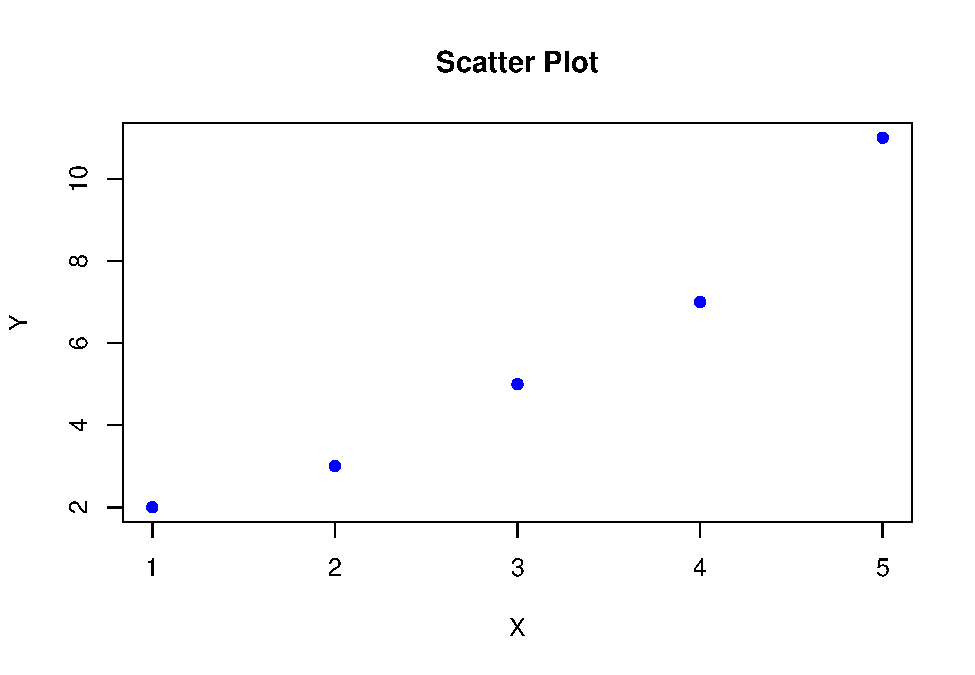
\includegraphics{_main_files/figure-latex/unnamed-chunk-25-1.pdf}

\begin{Shaded}
\begin{Highlighting}[]
\CommentTok{\# Create a line plot}
\FunctionTok{plot}\NormalTok{(x, y, }\AttributeTok{type =} \StringTok{"l"}\NormalTok{, }\AttributeTok{col =} \StringTok{"red"}\NormalTok{, }\AttributeTok{lwd =} \DecValTok{1}\NormalTok{, }\AttributeTok{main =} \StringTok{"Line plot"}\NormalTok{, }\AttributeTok{xlab =} \ConstantTok{NULL}\NormalTok{, }\AttributeTok{ylab =} \ConstantTok{NULL}\NormalTok{)}
\end{Highlighting}
\end{Shaded}

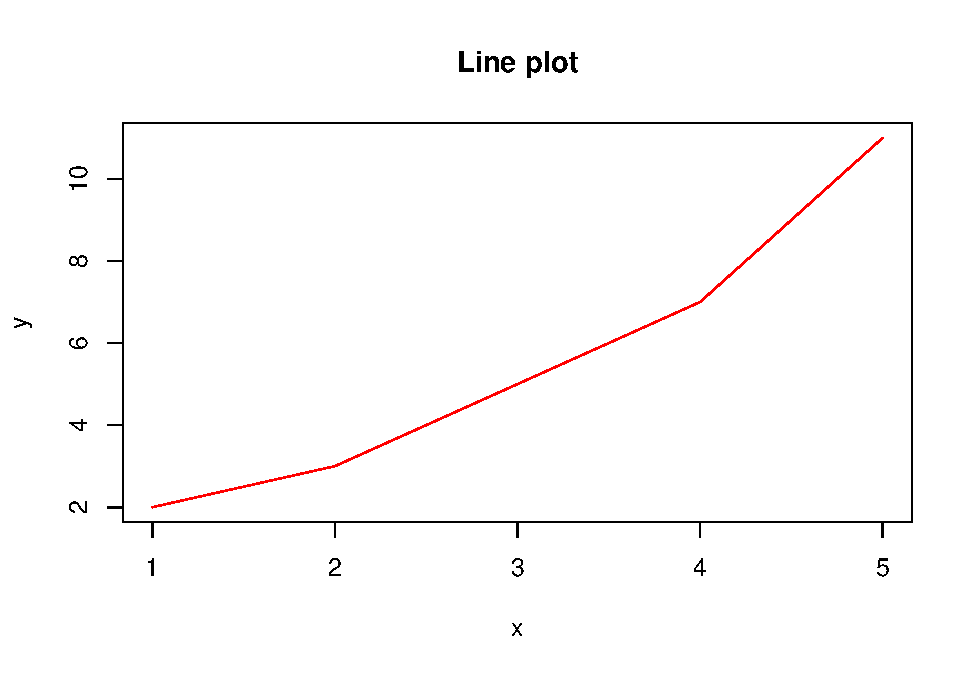
\includegraphics{_main_files/figure-latex/unnamed-chunk-25-2.pdf}

\subsection{Using hist() to create histograms for data distribution analysis}\label{using-hist-to-create-histograms-for-data-distribution-analysis}

Histograms are useful for visualizing the frequency distribution of a single variable. Similarly, you can get more documentation of the \textbf{hist()} function by running the command \textbf{?hist} in R. The generic function \textbf{hist} computes a histogram of the given data values.The default behavior for a histogram is to display frequencies on the vertical axis; probability densities can be displayed using the \textbf{freq=FALSE} option. The default title is given by \textbf{paste(``Histogram of'' , x)} where \textbf{x} is the name of the variable being plotted; this can be changed with the main option. The common syntax for the function is given below

\begin{Shaded}
\begin{Highlighting}[]
\CommentTok{\#hist(x, breaks = "Sturges",}
\CommentTok{\#     freq = NULL, probability = !freq,}
\CommentTok{\#     include.lowest = TRUE, right = TRUE, fuzz = 1e{-}7,}
\CommentTok{\#     density = NULL, angle = 45, col = "lightgray", border = NULL,}
\CommentTok{\#     main = paste("Histogram of" , xname),}
\CommentTok{\#     xlim = range(breaks), ylim = NULL,}
\CommentTok{\#     xlab = xname, ylab,}
\CommentTok{\#     axes = TRUE, plot = TRUE, labels = FALSE,}
\CommentTok{\#     nclass = NULL, warn.unused = TRUE, ...)}
\end{Highlighting}
\end{Shaded}

\begin{Shaded}
\begin{Highlighting}[]
\CommentTok{\# Create a histogram}
\FunctionTok{set.seed}\NormalTok{(}\DecValTok{100}\NormalTok{)  }\CommentTok{\# Fix the random numbers generated}
\NormalTok{data }\OtherTok{\textless{}{-}} \FunctionTok{rnorm}\NormalTok{(}\DecValTok{100}\NormalTok{)  }\CommentTok{\# Generate some random data}
\FunctionTok{hist}\NormalTok{(data, }\AttributeTok{breaks =} \StringTok{"Sturges"}\NormalTok{, }\AttributeTok{col =} \StringTok{"skyblue"}\NormalTok{, }\AttributeTok{main =} \StringTok{"Histogram"}\NormalTok{, }\AttributeTok{xlab =} \StringTok{"Value"}\NormalTok{, }\AttributeTok{ylab =} \StringTok{"Frequency"}\NormalTok{)}
\end{Highlighting}
\end{Shaded}

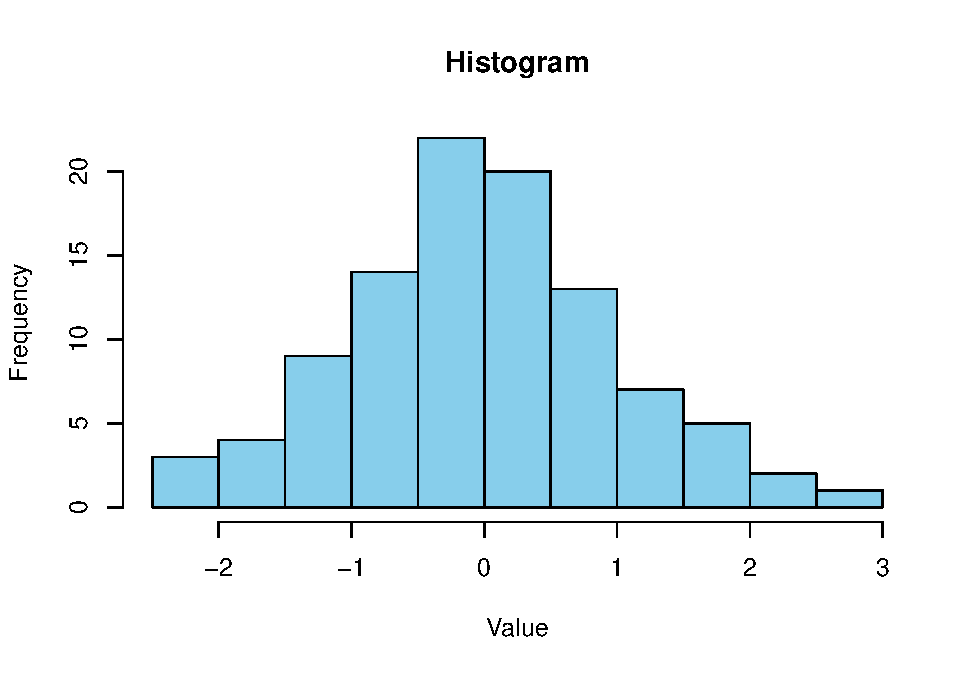
\includegraphics{_main_files/figure-latex/unnamed-chunk-27-1.pdf}

\subsection{Implementing boxplot() and barplot() to visualize data comparisons and distributions}\label{implementing-boxplot-and-barplot-to-visualize-data-comparisons-and-distributions}

The \textbf{boxplot()} and \textbf{barplot()} functions in R are commonly used for visualizing data comparisons and distributions.

\textbf{1. boxplot()}

The common syntax of the function is given below.

\begin{Shaded}
\begin{Highlighting}[]
\CommentTok{\#boxplot(x, data = NULL, col = "skyblue", main = NULL, xlab = NULL, ylab = \#NULL)}
\end{Highlighting}
\end{Shaded}

\textbf{Example}

\begin{Shaded}
\begin{Highlighting}[]
\CommentTok{\# Create a box plot}
\NormalTok{data }\OtherTok{\textless{}{-}} \FunctionTok{data.frame}\NormalTok{(}
  \AttributeTok{Group =} \FunctionTok{rep}\NormalTok{(}\FunctionTok{c}\NormalTok{(}\StringTok{"A"}\NormalTok{, }\StringTok{"B"}\NormalTok{, }\StringTok{"C"}\NormalTok{), }\AttributeTok{each =} \DecValTok{50}\NormalTok{),}
  \AttributeTok{Value =} \FunctionTok{c}\NormalTok{(}\FunctionTok{rnorm}\NormalTok{(}\DecValTok{50}\NormalTok{), }\FunctionTok{rnorm}\NormalTok{(}\DecValTok{50}\NormalTok{, }\AttributeTok{mean =} \DecValTok{2}\NormalTok{), }\FunctionTok{rnorm}\NormalTok{(}\DecValTok{50}\NormalTok{, }\AttributeTok{mean =} \DecValTok{3}\NormalTok{))}
\NormalTok{)}
\FunctionTok{boxplot}\NormalTok{(Value }\SpecialCharTok{\textasciitilde{}}\NormalTok{ Group, }\AttributeTok{data =}\NormalTok{ data, }\AttributeTok{col =} \StringTok{"skyblue"}\NormalTok{, }\AttributeTok{main =} \StringTok{"Box Plot"}\NormalTok{, }\AttributeTok{xlab =} \StringTok{"Group"}\NormalTok{, }\AttributeTok{ylab =} \StringTok{"Value"}\NormalTok{)}
\end{Highlighting}
\end{Shaded}

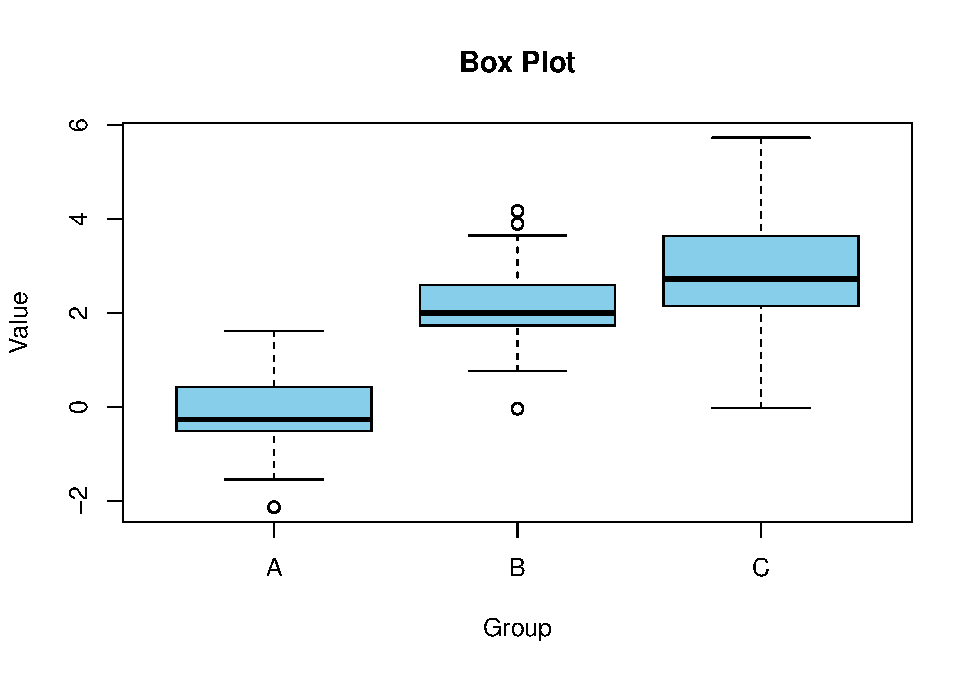
\includegraphics{_main_files/figure-latex/unnamed-chunk-29-1.pdf}

\textbf{2.barplot()}
The syntax used for \textbf{barplot()} function is given below.

\begin{Shaded}
\begin{Highlighting}[]
\CommentTok{\#barplot(x, names.arg = NULL, col = "skyblue", main = NULL, xlab = NULL, \#ylab = NULL)}
\end{Highlighting}
\end{Shaded}

\textbf{Example}

\begin{Shaded}
\begin{Highlighting}[]
\CommentTok{\# Create a bar plot}
\NormalTok{data }\OtherTok{\textless{}{-}} \FunctionTok{table}\NormalTok{(mtcars}\SpecialCharTok{$}\NormalTok{cyl)}
\FunctionTok{barplot}\NormalTok{(data, }\AttributeTok{col =} \StringTok{"skyblue"}\NormalTok{, }\AttributeTok{main =} \StringTok{"Bar Plot"}\NormalTok{, }\AttributeTok{xlab =} \StringTok{"Number of Cylinders"}\NormalTok{, }\AttributeTok{ylab =} \StringTok{"Frequency"}\NormalTok{)}
\end{Highlighting}
\end{Shaded}

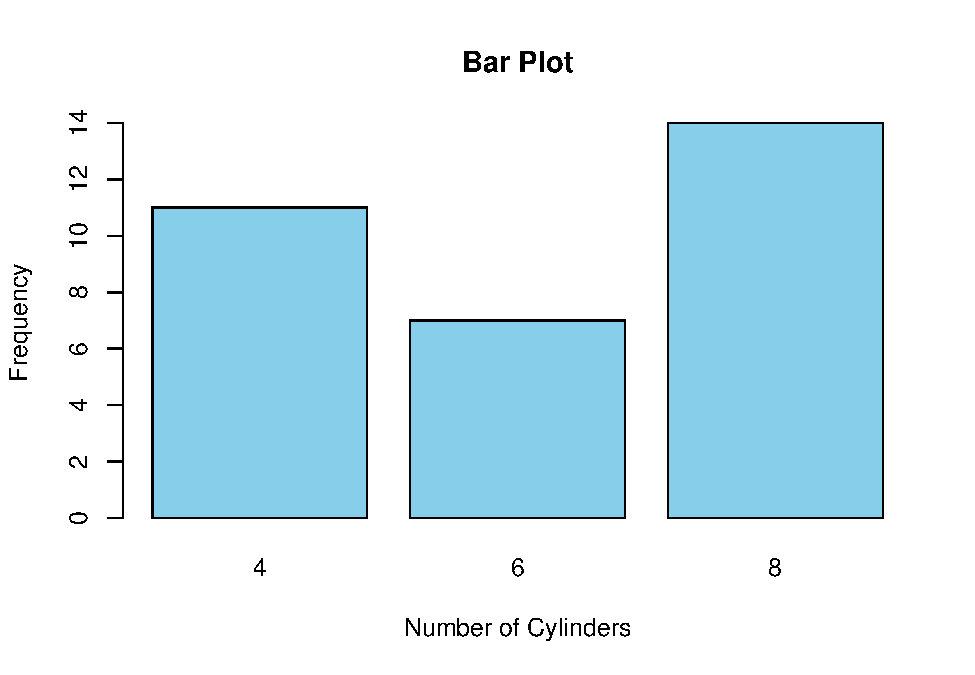
\includegraphics{_main_files/figure-latex/unnamed-chunk-31-1.pdf}

\section{Customizing Plots}\label{customizing-plots}

\subsection{Basic customization options including colors, main titles, axis labels, and plot dimensions}\label{basic-customization-options-including-colors-main-titles-axis-labels-and-plot-dimensions}

\textbf{1. Changing Colors}

\begin{Shaded}
\begin{Highlighting}[]
\CommentTok{\# Create a scatter plot with custom colors}
\NormalTok{x }\OtherTok{\textless{}{-}} \FunctionTok{c}\NormalTok{(}\DecValTok{1}\NormalTok{, }\DecValTok{2}\NormalTok{, }\DecValTok{3}\NormalTok{, }\DecValTok{4}\NormalTok{, }\DecValTok{5}\NormalTok{)}
\NormalTok{y }\OtherTok{\textless{}{-}} \FunctionTok{c}\NormalTok{(}\DecValTok{2}\NormalTok{, }\DecValTok{3}\NormalTok{, }\DecValTok{5}\NormalTok{, }\DecValTok{7}\NormalTok{, }\DecValTok{11}\NormalTok{)}
\FunctionTok{plot}\NormalTok{(x, y, }\AttributeTok{type =} \StringTok{"p"}\NormalTok{, }\AttributeTok{col =} \StringTok{"red"}\NormalTok{, }\AttributeTok{pch =} \DecValTok{16}\NormalTok{, }\AttributeTok{main =} \StringTok{""}\NormalTok{, }\AttributeTok{xlab =} \StringTok{"X"}\NormalTok{, }\AttributeTok{ylab =} \StringTok{"Y"}\NormalTok{)}
\end{Highlighting}
\end{Shaded}

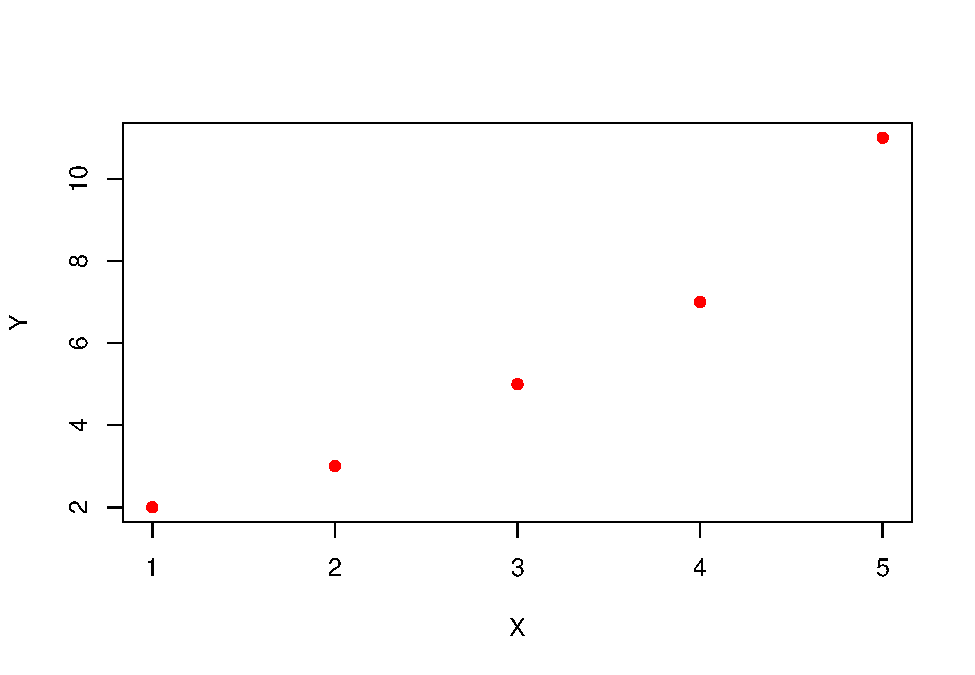
\includegraphics{_main_files/figure-latex/unnamed-chunk-32-1.pdf}

\textbf{2. Adding Titles and Axis Labels}

\begin{Shaded}
\begin{Highlighting}[]
\CommentTok{\# Create a scatter plot with titles and axis labels}
\NormalTok{x }\OtherTok{\textless{}{-}} \FunctionTok{c}\NormalTok{(}\DecValTok{1}\NormalTok{, }\DecValTok{2}\NormalTok{, }\DecValTok{3}\NormalTok{, }\DecValTok{4}\NormalTok{, }\DecValTok{5}\NormalTok{)}
\NormalTok{y }\OtherTok{\textless{}{-}} \FunctionTok{c}\NormalTok{(}\DecValTok{2}\NormalTok{, }\DecValTok{3}\NormalTok{, }\DecValTok{5}\NormalTok{, }\DecValTok{7}\NormalTok{, }\DecValTok{11}\NormalTok{)}
\FunctionTok{plot}\NormalTok{(x, y, }\AttributeTok{type =} \StringTok{"p"}\NormalTok{, }\AttributeTok{col =} \StringTok{"red"}\NormalTok{, }\AttributeTok{pch =} \DecValTok{16}\NormalTok{, }\AttributeTok{main =} \StringTok{"Scatter Plot"}\NormalTok{, }\AttributeTok{xlab =} \StringTok{"X{-}axis"}\NormalTok{, }\AttributeTok{ylab =} \StringTok{"Y{-}axis"}\NormalTok{)}
\end{Highlighting}
\end{Shaded}

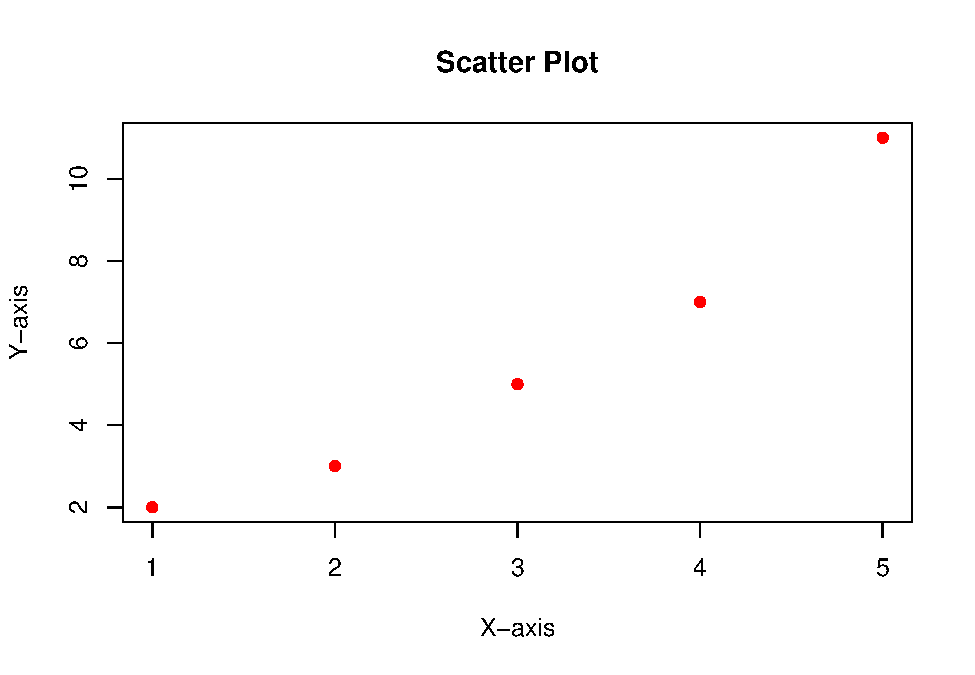
\includegraphics{_main_files/figure-latex/unnamed-chunk-33-1.pdf}

\textbf{3. Changing Plot Dimensions}

\begin{Shaded}
\begin{Highlighting}[]
\CommentTok{\# Create a scatter plot with custom dimensions}
\NormalTok{x }\OtherTok{\textless{}{-}} \FunctionTok{c}\NormalTok{(}\DecValTok{1}\NormalTok{, }\DecValTok{2}\NormalTok{, }\DecValTok{3}\NormalTok{, }\DecValTok{4}\NormalTok{, }\DecValTok{5}\NormalTok{)}
\NormalTok{y }\OtherTok{\textless{}{-}} \FunctionTok{c}\NormalTok{(}\DecValTok{2}\NormalTok{, }\DecValTok{3}\NormalTok{, }\DecValTok{5}\NormalTok{, }\DecValTok{7}\NormalTok{, }\DecValTok{11}\NormalTok{)}
\FunctionTok{plot}\NormalTok{(x, y, }\AttributeTok{type =} \StringTok{"p"}\NormalTok{, }\AttributeTok{col =} \StringTok{"red"}\NormalTok{, }\AttributeTok{pch =} \DecValTok{16}\NormalTok{, }\AttributeTok{main =} \StringTok{"Scatter Plot"}\NormalTok{, }\AttributeTok{xlab =} \StringTok{"X"}\NormalTok{, }\AttributeTok{ylab =} \StringTok{"Y"}\NormalTok{, }\AttributeTok{xlim =} \FunctionTok{c}\NormalTok{(}\DecValTok{0}\NormalTok{, }\DecValTok{6}\NormalTok{), }\AttributeTok{ylim =} \FunctionTok{c}\NormalTok{(}\DecValTok{0}\NormalTok{, }\DecValTok{12}\NormalTok{))}
\end{Highlighting}
\end{Shaded}

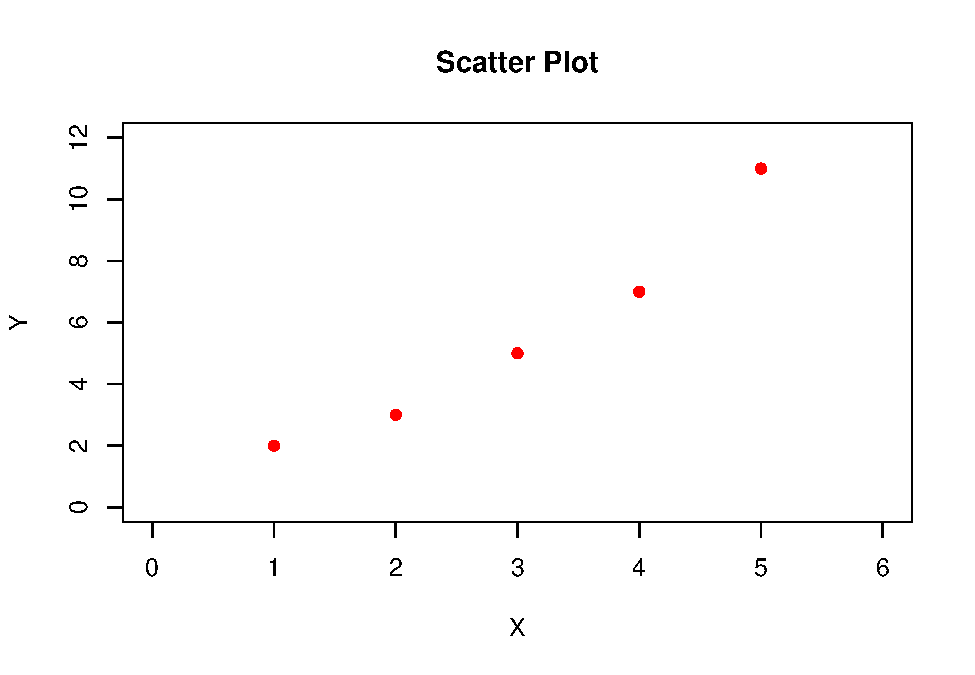
\includegraphics{_main_files/figure-latex/unnamed-chunk-34-1.pdf}

\textbf{4. Combining Customization Options}

\begin{Shaded}
\begin{Highlighting}[]
\CommentTok{\# Create a scatter plot with custom colors, titles, axis labels, and dimensions}
\NormalTok{x }\OtherTok{\textless{}{-}} \FunctionTok{c}\NormalTok{(}\DecValTok{1}\NormalTok{, }\DecValTok{2}\NormalTok{, }\DecValTok{3}\NormalTok{, }\DecValTok{4}\NormalTok{, }\DecValTok{5}\NormalTok{)}
\NormalTok{y }\OtherTok{\textless{}{-}} \FunctionTok{c}\NormalTok{(}\DecValTok{2}\NormalTok{, }\DecValTok{3}\NormalTok{, }\DecValTok{5}\NormalTok{, }\DecValTok{7}\NormalTok{, }\DecValTok{11}\NormalTok{)}
\FunctionTok{plot}\NormalTok{(x, y, }\AttributeTok{type =} \StringTok{"p"}\NormalTok{, }\AttributeTok{col =} \StringTok{"red"}\NormalTok{, }\AttributeTok{pch =} \DecValTok{16}\NormalTok{, }\AttributeTok{main =} \StringTok{"Scatter Plot"}\NormalTok{, }\AttributeTok{xlab =} \StringTok{"X{-}axis"}\NormalTok{, }\AttributeTok{ylab =} \StringTok{"Y{-}axis"}\NormalTok{, }\AttributeTok{xlim =} \FunctionTok{c}\NormalTok{(}\DecValTok{0}\NormalTok{, }\DecValTok{6}\NormalTok{), }\AttributeTok{ylim =} \FunctionTok{c}\NormalTok{(}\DecValTok{0}\NormalTok{, }\DecValTok{12}\NormalTok{))}
\end{Highlighting}
\end{Shaded}

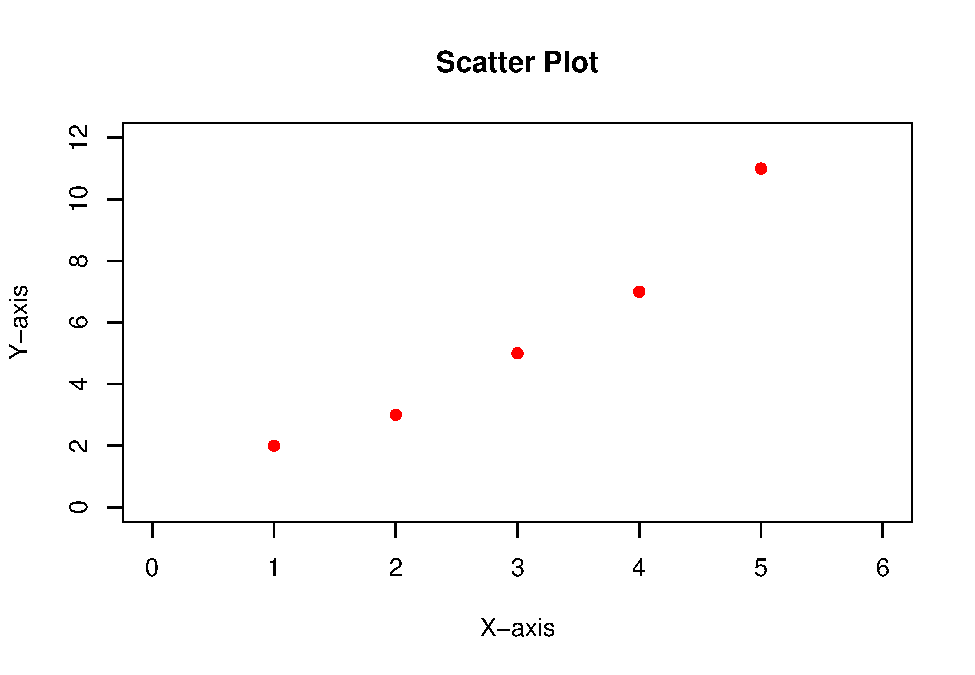
\includegraphics{_main_files/figure-latex/unnamed-chunk-35-1.pdf}

You can further customize your plots by adjusting parameters such as \textbf{pch} (for points), \textbf{lwd} (for lines), \textbf{lty} (for line type), \textbf{cex} (for point size), and more.

\subsection{Tips on enhancing plot readability and aesthetic appeal}\label{tips-on-enhancing-plot-readability-and-aesthetic-appeal}

In order to have a plot with enhanced readability and have an aesthetic appeal, you need to use some of these tips:

\begin{itemize}
\tightlist
\item
  \textbf{Choose appropriate colors:} Use colors that complement each other and make it easy to distinguish different elements of the plot.Avoid using colors that are too bright or too similar to each other.
\item
  \textbf{Use appropriate font sizes and styles:} Use larger font sizes for titles and axis labels to make them more prominent.
\item
  \textbf{Add grid lines:} Adding grid lines can make it easier to read the plot and interpret the data.
\item
  \textbf{Use appropriate plot types:} Choose the appropriate plot type for your data. For example, use a scatter plot for continuous data and a bar plot for categorical data.
\item
  \textbf{Use consistent and intuitive labeling:} Make sure that the labels on your plot are consistent and intuitive, making it easy for readers to understand the information presented.
\item
  \textbf{Use legends for clarity:} Use legends to explain the meaning of different colors or symbols used in the plot.
\end{itemize}

You can also add more improvements to your plot to make it look more nice and appealing.

\section{Practical Examples: Exercises}\label{practical-examples-exercises-1}

\textbf{Exercise 6}

Create a dataframe of marks of 1000 students (male and female) with their respective status i.e pass if marks \textgreater= 40, fail otherwise (set a seed to 100). Additionally, let the student marks be graded using factor method in the following format:

A: 70 marks and above

B: 60-69

C: 50-59

D: 40-49

E: Below 40 marks

Create a dataframe called students with the vectors; id, gender, marks, grade and status where status is a column which shows whether the student passed or failed.You will use this dataframe to answer exercise 7,8 and 9.

\begin{Shaded}
\begin{Highlighting}[]
\CommentTok{\# Your code}
\end{Highlighting}
\end{Shaded}

\textbf{Exercise 7}

Plot a box plot to show the distribution of marks by gender.Give it a title, `Distribution of Student Marks'. The x-axis should be labelled as `Gender' while the y-axis should be labelled as `Marks'. Apply blue color to male and green color to female. Set cex.main and cex.lab to 1.2.

\begin{Shaded}
\begin{Highlighting}[]
\CommentTok{\#Your code}
\end{Highlighting}
\end{Shaded}

\textbf{Exercise 8}

Plot a histogram of the marks where the bins should be equivalent to the classes of grading. Which grade had the highest number of students? How were the marks distributed in the class? Fill the histogram with red. Add a customized title and label the axes.

\begin{Shaded}
\begin{Highlighting}[]
\CommentTok{\#Your code}
\end{Highlighting}
\end{Shaded}

\textbf{Exercise 9}

Use a well customized barpot to show the mean mark of students by gender. Which gender had the highest average score?

\begin{Shaded}
\begin{Highlighting}[]
\CommentTok{\#Your code}
\end{Highlighting}
\end{Shaded}

\chapter{DATA STRUCTURES RELEVANT TO VISUALIZATION}\label{data-structures-relevant-to-visualization}

\section{Introduction}\label{introduction-1}

The two main objectives of this chapter is to understand various data structures in R and learn how to manipulate and prepare data for effective visualization.

Understanding data structures is crucial for creating effective visualizations in R. Properly organizing and structuring your data allows you to generate clear and insightful visual outputs. In this chapter, we will discuss the importance of data structure understanding in achieving effective visualizations.

\subsection{Importance of Data Structure Understanding}\label{importance-of-data-structure-understanding}

\begin{itemize}
\tightlist
\item
  \textbf{Data Compatibility:} Different types of visualizations require different data structures. Understanding how to structure your data properly ensures compatibility with the visualization techniques you want to use.
\item
  \textbf{Efficient Data Handling:} Well-structured data is easier to manipulate and process, leading to more efficient visualization workflows.
\item
  \textbf{Insightful Visual Outputs:} Properly structured data enables you to generate visual outputs that effectively communicate your insights and findings.
\end{itemize}

The most commonly used data structures for visualization are vectors, matrices, data frames and lists.

\section{Vectors, Data Frames, and Matrices}\label{vectors-data-frames-and-matrices}

\subsection{Definitions}\label{definitions}

\textbf{Vectors} are one-dimensional arrays that can hold numeric, character, or logical values. They are suitable for creating simple plots like scatter plots and line graphs. For example, a vector of numeric values can be used to represent data on the x or y-axis of a plot.

A \textbf{data frame} is a two-dimensional data structure where columns can be of different types. Data frames are highly versatile and commonly used for data analysis and visualization. They are suitable for creating a wide range of visualizations, including bar plots, histograms, and box plots. Each column in a data frame can represent a different variable, making it easy to visualize relationships between variables.

\textbf{Matrices} are two-dimensional arrays that contain elements of the same atomic types. Matrices are useful for creating visualizations such as heatmaps and surface plots. They are suitable for representing data that has two dimensions, such as images or spatial data.

\textbf{Lists} are ordered collections of objects, which can be of different types. Lists can also be nested, allowing for complex data structures. They provide flexibility in organizing and storing data for complex visualizations. They are suitable for creating custom plots or combining multiple plots into a single visualization.

\textbf{Factors} are used to represent categorical data in R. They are stored as integers and have labels associated with them. They are useful for creating plots that involve categorical data, such as bar plots and pie charts. They allow for easy grouping and aggregation of data based on categorical variables.

\textbf{Example}

\begin{Shaded}
\begin{Highlighting}[]
\CommentTok{\# Example data}
\FunctionTok{set.seed}\NormalTok{(}\DecValTok{123}\NormalTok{)}
\NormalTok{numeric\_vector }\OtherTok{\textless{}{-}} \FunctionTok{rnorm}\NormalTok{(}\DecValTok{10}\NormalTok{)}
\NormalTok{character\_vector }\OtherTok{\textless{}{-}}\NormalTok{ letters[}\DecValTok{1}\SpecialCharTok{:}\DecValTok{10}\NormalTok{]}
\NormalTok{logical\_vector }\OtherTok{\textless{}{-}} \FunctionTok{sample}\NormalTok{(}\FunctionTok{c}\NormalTok{(}\ConstantTok{TRUE}\NormalTok{, }\ConstantTok{FALSE}\NormalTok{), }\DecValTok{10}\NormalTok{, }\AttributeTok{replace =} \ConstantTok{TRUE}\NormalTok{)}

\CommentTok{\# Create a list}
\NormalTok{my\_list }\OtherTok{\textless{}{-}} \FunctionTok{list}\NormalTok{(numeric\_vector, character\_vector, logical\_vector)}

\CommentTok{\# Create a matrix}
\NormalTok{my\_matrix }\OtherTok{\textless{}{-}} \FunctionTok{matrix}\NormalTok{(}\DecValTok{1}\SpecialCharTok{:}\DecValTok{12}\NormalTok{, }\AttributeTok{nrow =} \DecValTok{4}\NormalTok{)}

\CommentTok{\# Create a data frame}
\NormalTok{my\_data }\OtherTok{\textless{}{-}} \FunctionTok{data.frame}\NormalTok{(}
  \AttributeTok{ID =} \DecValTok{1}\SpecialCharTok{:}\DecValTok{4}\NormalTok{,}
  \AttributeTok{Name =} \FunctionTok{c}\NormalTok{(}\StringTok{"John"}\NormalTok{, }\StringTok{"Mary"}\NormalTok{, }\StringTok{"David"}\NormalTok{, }\StringTok{"Emma"}\NormalTok{),}
  \AttributeTok{Age =} \FunctionTok{c}\NormalTok{(}\DecValTok{25}\NormalTok{, }\DecValTok{30}\NormalTok{, }\DecValTok{35}\NormalTok{, }\DecValTok{40}\NormalTok{)}
\NormalTok{)}

\CommentTok{\# Create a factor}
\NormalTok{my\_factor }\OtherTok{\textless{}{-}} \FunctionTok{factor}\NormalTok{(}\FunctionTok{c}\NormalTok{(}\StringTok{"A"}\NormalTok{, }\StringTok{"B"}\NormalTok{, }\StringTok{"A"}\NormalTok{, }\StringTok{"C"}\NormalTok{))}

\CommentTok{\# Print the structures}
\FunctionTok{print}\NormalTok{(my\_list)}
\end{Highlighting}
\end{Shaded}

\begin{verbatim}
## [[1]]
##  [1] -0.56047565 -0.23017749  1.55870831  0.07050839  0.12928774  1.71506499
##  [7]  0.46091621 -1.26506123 -0.68685285 -0.44566197
## 
## [[2]]
##  [1] "a" "b" "c" "d" "e" "f" "g" "h" "i" "j"
## 
## [[3]]
##  [1]  TRUE FALSE  TRUE  TRUE  TRUE  TRUE FALSE FALSE  TRUE FALSE
\end{verbatim}

\begin{Shaded}
\begin{Highlighting}[]
\FunctionTok{print}\NormalTok{(my\_matrix)}
\end{Highlighting}
\end{Shaded}

\begin{verbatim}
##      [,1] [,2] [,3]
## [1,]    1    5    9
## [2,]    2    6   10
## [3,]    3    7   11
## [4,]    4    8   12
\end{verbatim}

\begin{Shaded}
\begin{Highlighting}[]
\FunctionTok{print}\NormalTok{(my\_data)}
\end{Highlighting}
\end{Shaded}

\begin{verbatim}
##   ID  Name Age
## 1  1  John  25
## 2  2  Mary  30
## 3  3 David  35
## 4  4  Emma  40
\end{verbatim}

\begin{Shaded}
\begin{Highlighting}[]
\FunctionTok{print}\NormalTok{(my\_factor)}
\end{Highlighting}
\end{Shaded}

\begin{verbatim}
## [1] A B A C
## Levels: A B C
\end{verbatim}

\subsection{Tools and Functions}\label{tools-and-functions}

Understanding various tools and functions in R is essential for manipulating data structures effectively. Here are some commonly used tools and functions:

\textbf{1. str():} Displays the internal structure of R objects. For example if the object is a data frame, it shows the type of each vector in the dataframe

\textbf{2. class():} Returns the class of the R object.

\textbf{3. length():} Returns the number of elements in the R object. If the object is a data frame, it returns the number of columns in the data frame.

\textbf{4. dim():} Returns the dimensions of an R object (for matrices and arrays).

\textbf{5. attributes():} Returns the attributes of an R object.

\textbf{6. as.factor():} Converts a vector to a factor.

\textbf{7. data.frame():} Creates a data frame from vectors or other R objects.

\textbf{8. ncol():} Returns the number of columns of a dataframe or matrix.

\textbf{9. nrow():} Returns the number of rows of a data frame.

\subsection{Step-by-Step Tutorials}\label{step-by-step-tutorials}

\subsubsection{Converting a Vector to a Data Frame}\label{converting-a-vector-to-a-data-frame}

\begin{Shaded}
\begin{Highlighting}[]
\CommentTok{\# Example vector}
\NormalTok{student\_id }\OtherTok{\textless{}{-}} \DecValTok{1}\SpecialCharTok{:}\DecValTok{5}
\NormalTok{student\_name }\OtherTok{\textless{}{-}} \FunctionTok{c}\NormalTok{(}\StringTok{"John"}\NormalTok{, }\StringTok{"Alice"}\NormalTok{, }\StringTok{"Bob"}\NormalTok{, }\StringTok{"Emily"}\NormalTok{, }\StringTok{"Tom"}\NormalTok{)}
\NormalTok{student\_score }\OtherTok{\textless{}{-}} \FunctionTok{c}\NormalTok{(}\DecValTok{80}\NormalTok{, }\DecValTok{75}\NormalTok{, }\DecValTok{90}\NormalTok{, }\DecValTok{85}\NormalTok{, }\DecValTok{88}\NormalTok{)}

\CommentTok{\# Combine vectors into a data frame}
\NormalTok{student\_data }\OtherTok{\textless{}{-}} \FunctionTok{data.frame}\NormalTok{(}\AttributeTok{ID =}\NormalTok{ student\_id, }\AttributeTok{Name =}\NormalTok{ student\_name, }\AttributeTok{Score =}\NormalTok{ student\_score)}

\CommentTok{\# View the data frame}
\FunctionTok{print}\NormalTok{(student\_data)}
\end{Highlighting}
\end{Shaded}

\begin{verbatim}
##   ID  Name Score
## 1  1  John    80
## 2  2 Alice    75
## 3  3   Bob    90
## 4  4 Emily    85
## 5  5   Tom    88
\end{verbatim}

\subsubsection{Creating and Modifying Lists for Nested Data Structures}\label{creating-and-modifying-lists-for-nested-data-structures}

\begin{Shaded}
\begin{Highlighting}[]
\CommentTok{\# Example list}
\NormalTok{student1 }\OtherTok{\textless{}{-}} \FunctionTok{list}\NormalTok{(}\AttributeTok{Name =} \StringTok{"John"}\NormalTok{, }\AttributeTok{Age =} \DecValTok{25}\NormalTok{, }\AttributeTok{Grades =} \FunctionTok{c}\NormalTok{(}\AttributeTok{Math =} \DecValTok{80}\NormalTok{, }\AttributeTok{Science =} \DecValTok{85}\NormalTok{))}
\NormalTok{student2 }\OtherTok{\textless{}{-}} \FunctionTok{list}\NormalTok{(}\AttributeTok{Name =} \StringTok{"Alice"}\NormalTok{, }\AttributeTok{Age =} \DecValTok{23}\NormalTok{, }\AttributeTok{Grades =} \FunctionTok{c}\NormalTok{(}\AttributeTok{Math =} \DecValTok{75}\NormalTok{, }\AttributeTok{Science =} \DecValTok{78}\NormalTok{))}

\CommentTok{\# Create a nested list}
\NormalTok{classroom }\OtherTok{\textless{}{-}} \FunctionTok{list}\NormalTok{(student1, student2)}

\CommentTok{\# View the nested list}
\FunctionTok{print}\NormalTok{(classroom)}
\end{Highlighting}
\end{Shaded}

\begin{verbatim}
## [[1]]
## [[1]]$Name
## [1] "John"
## 
## [[1]]$Age
## [1] 25
## 
## [[1]]$Grades
##    Math Science 
##      80      85 
## 
## 
## [[2]]
## [[2]]$Name
## [1] "Alice"
## 
## [[2]]$Age
## [1] 23
## 
## [[2]]$Grades
##    Math Science 
##      75      78
\end{verbatim}

\begin{Shaded}
\begin{Highlighting}[]
\CommentTok{\# Accessing elements of the nested list}
\FunctionTok{print}\NormalTok{(classroom[[}\DecValTok{1}\NormalTok{]]}\SpecialCharTok{$}\NormalTok{Name)  }\CommentTok{\# Output: John}
\end{Highlighting}
\end{Shaded}

\begin{verbatim}
## [1] "John"
\end{verbatim}

\begin{Shaded}
\begin{Highlighting}[]
\FunctionTok{print}\NormalTok{(classroom[[}\DecValTok{2}\NormalTok{]]}\SpecialCharTok{$}\NormalTok{Grades[}\StringTok{"Science"}\NormalTok{])  }\CommentTok{\# Output: 78}
\end{Highlighting}
\end{Shaded}

\begin{verbatim}
## Science 
##      78
\end{verbatim}

\begin{Shaded}
\begin{Highlighting}[]
\CommentTok{\# Modifying elements of the nested list}
\NormalTok{classroom[[}\DecValTok{1}\NormalTok{]]}\SpecialCharTok{$}\NormalTok{Grades[}\StringTok{"Math"}\NormalTok{] }\OtherTok{\textless{}{-}} \DecValTok{85}

\CommentTok{\# View the modified nested list}
\FunctionTok{print}\NormalTok{(classroom)}
\end{Highlighting}
\end{Shaded}

\begin{verbatim}
## [[1]]
## [[1]]$Name
## [1] "John"
## 
## [[1]]$Age
## [1] 25
## 
## [[1]]$Grades
##    Math Science 
##      85      85 
## 
## 
## [[2]]
## [[2]]$Name
## [1] "Alice"
## 
## [[2]]$Age
## [1] 23
## 
## [[2]]$Grades
##    Math Science 
##      75      78
\end{verbatim}

\section{Practical Example : Exercise}\label{practical-example-exercise}

\textbf{Exercise 10}

You have been provided with a snapshot of a fictional retail landscape, capturing essential attributes that drive retail operations and customer interactions. It includes key details such as Transaction ID, Date, Customer ID, Gender, Age, Product Category, Quantity, Price per Unit, and Total Amount. The dataset can be downloaded from Kaggle via the link \url{https://www.kaggle.com/datasets/mohammadtalib786/retail-sales-dataset}. Import the data into R and answer the following questions:

i). Using a well customized line plot, what trend do you see in the sales (Total Amount)?

ii). Using an appropriate plot covered so far, show how the total amount vary by the product category. Use a well customized plot to make it more appealing and readable.

\chapter{CUSTOMIZING GRAPHS IN BASE R}\label{customizing-graphs-in-base-r}

\section{Introduction}\label{introduction-2}

The main objectives of this chapter are:

\begin{itemize}
\tightlist
\item
  Learn to customize and enhance graphs using R's base graphic parameters.
\item
  Understand how to apply visual enhancements to convey information more
  effectively.
\end{itemize}

\section{Graph Customization Basics}\label{graph-customization-basics}

Customizing plots in R allows you to enhance the appearance and readability of the visualizations. The \textbf{par()} function in R is used to set or query graphical parameters.

\textbf{i). Graphical Parameters (par())}

\begin{itemize}
\tightlist
\item
  \textbf{pch:} Sets the plotting symbol (or point character) used in plotting functions like \textbf{plot()}.
\item
  \textbf{lty:} Sets the line type.
\item
  \textbf{lwd:} Sets the line width.
\item
  \textbf{col:} Sets the color of lines and points.
\item
  \textbf{bg:} Sets the background color.
\item
  \textbf{cex:} Sets the character size.
\item
  \textbf{mar:} Sets the margins of the plot.
\end{itemize}

\textbf{ii). Adding Custom Colors, Line Types, Point Shapes, and Plot Characters}

\begin{itemize}
\tightlist
\item
  \textbf{Custom Colors:} You can specify custom colors using color names, hexadecimal codes, or color numbers.
\item
  \textbf{Line Types:} Different line types are available, such as solid, dashed, dotted, etc.
\item
  \textbf{Point Shapes:} Various point shapes are available, including circles, squares, triangles, etc.
\item
  \textbf{Plot Characters:} Different plot characters, such as dots, crosses, stars, etc., can be used.
\end{itemize}

\textbf{Example:}

\begin{Shaded}
\begin{Highlighting}[]
\CommentTok{\# Sample data}
\NormalTok{x }\OtherTok{\textless{}{-}} \DecValTok{1}\SpecialCharTok{:}\DecValTok{10}
\NormalTok{y }\OtherTok{\textless{}{-}}\NormalTok{ x}\SpecialCharTok{\^{}}\DecValTok{2}

\CommentTok{\# Plot with customized graphical parameters}
\FunctionTok{par}\NormalTok{(}
  \AttributeTok{pch =} \DecValTok{19}\NormalTok{,    }\CommentTok{\# Use solid circles for points}
  \AttributeTok{lty =} \DecValTok{2}\NormalTok{,     }\CommentTok{\# Use dashed line}
  \AttributeTok{lwd =} \DecValTok{2}\NormalTok{,     }\CommentTok{\# Set line width to 2}
  \AttributeTok{col =} \StringTok{"blue"} \CommentTok{\# Set line and point color to blue}
\NormalTok{)}

\FunctionTok{plot}\NormalTok{(x, y, }\AttributeTok{type =} \StringTok{"l"}\NormalTok{, }\AttributeTok{main =} \StringTok{"Customized Plot"}\NormalTok{, }\AttributeTok{xlab =} \StringTok{"X"}\NormalTok{, }\AttributeTok{ylab =} \StringTok{"Y"}\NormalTok{)}
\FunctionTok{points}\NormalTok{(x, y, }\AttributeTok{col =} \StringTok{"red"}\NormalTok{) }\CommentTok{\# Add points with red color}
\end{Highlighting}
\end{Shaded}

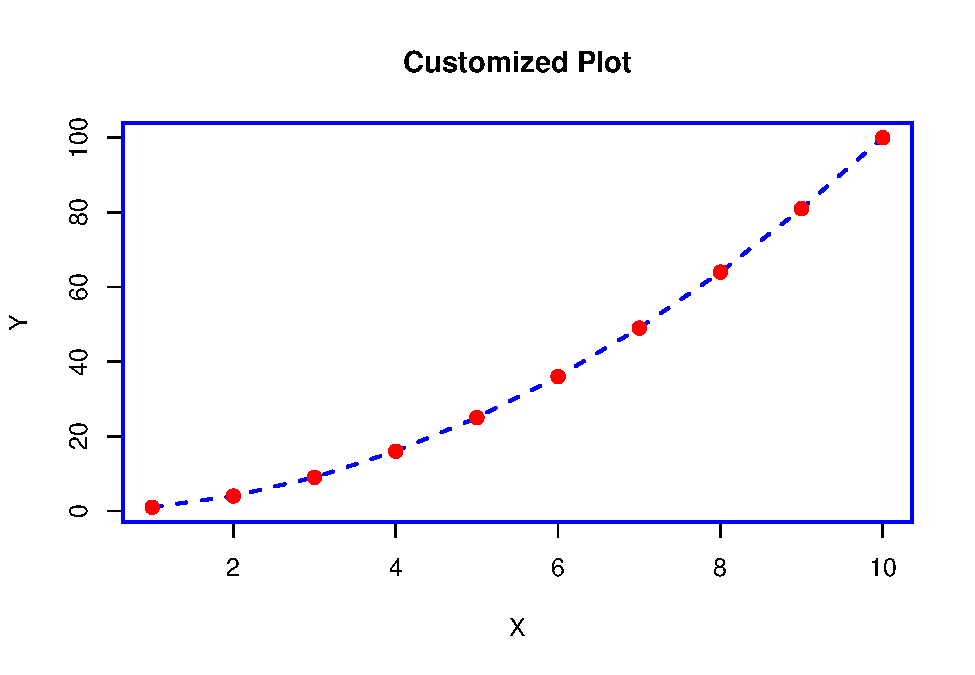
\includegraphics{_main_files/figure-latex/unnamed-chunk-45-1.pdf}

\section{Enhancing Plot Aesthetics}\label{enhancing-plot-aesthetics}

Improving the aesthetics of plots is essential for effectively communicating your data. The following are some techniques for enhancing plot aesthetics in R:

\textbf{1. Setting Axis Options:}

\textbf{Axis Labels:} Use \textbf{xlab} and \textbf{ylab} parameters to set labels for x and y axes, respectively.

\textbf{Tick Marks:} Use \textbf{axes = FALSE} to remove axis tick marks and add them back using axis() function.

\textbf{Axis Limits:} Use \textbf{xlim} and \textbf{ylim} parameters to set limits for the x and y axes, respectively.

Example:

\begin{Shaded}
\begin{Highlighting}[]
\CommentTok{\# Sample data}
\NormalTok{x }\OtherTok{\textless{}{-}} \DecValTok{1}\SpecialCharTok{:}\DecValTok{10}
\NormalTok{y }\OtherTok{\textless{}{-}}\NormalTok{ x}\SpecialCharTok{\^{}}\DecValTok{2}

\CommentTok{\# Plot with customized axis options}
\FunctionTok{plot}\NormalTok{(x, y, }\AttributeTok{type =} \StringTok{"l"}\NormalTok{, }\AttributeTok{main =} \StringTok{"A simple line plot"}\NormalTok{, }\AttributeTok{xlab =} \StringTok{"X{-}axis"}\NormalTok{, }\AttributeTok{ylab =} \StringTok{"Y{-}axis"}\NormalTok{, }\AttributeTok{xlim =} \FunctionTok{c}\NormalTok{(}\DecValTok{0}\NormalTok{, }\DecValTok{12}\NormalTok{), }\AttributeTok{ylim =} \FunctionTok{c}\NormalTok{(}\DecValTok{0}\NormalTok{, }\DecValTok{120}\NormalTok{))}
\FunctionTok{axis}\NormalTok{(}\AttributeTok{side =} \DecValTok{1}\NormalTok{, }\AttributeTok{at =} \FunctionTok{seq}\NormalTok{(}\DecValTok{0}\NormalTok{, }\DecValTok{12}\NormalTok{, }\AttributeTok{by =} \DecValTok{2}\NormalTok{)) }\CommentTok{\# Add x{-}axis tick marks}
\FunctionTok{axis}\NormalTok{(}\AttributeTok{side =} \DecValTok{2}\NormalTok{, }\AttributeTok{at =} \FunctionTok{seq}\NormalTok{(}\DecValTok{0}\NormalTok{, }\DecValTok{120}\NormalTok{, }\AttributeTok{by =} \DecValTok{20}\NormalTok{)) }\CommentTok{\# Add y{-}axis tick marks}
\end{Highlighting}
\end{Shaded}

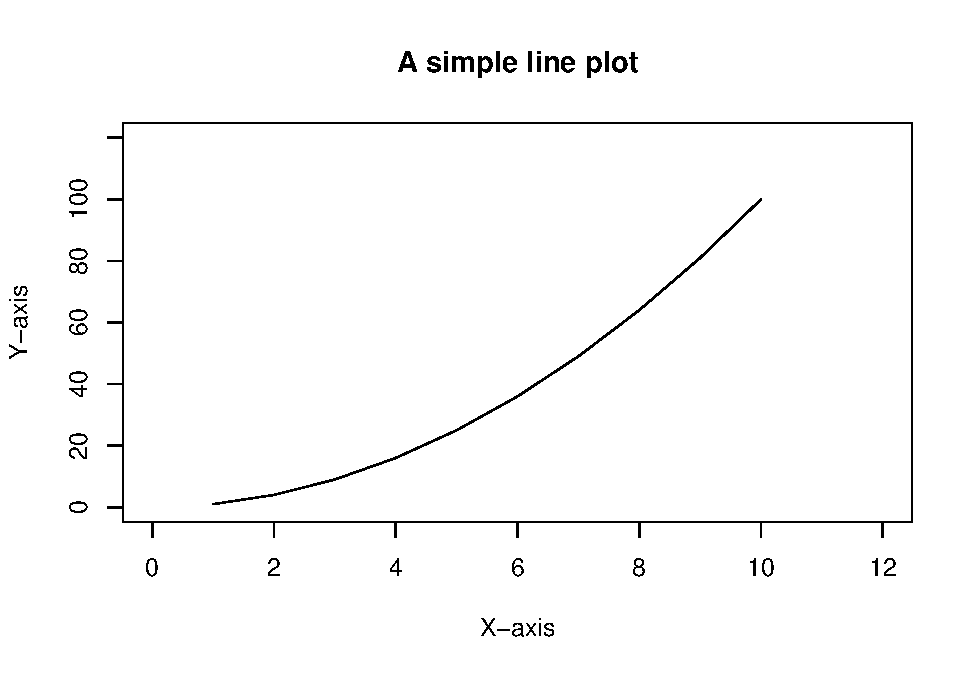
\includegraphics{_main_files/figure-latex/unnamed-chunk-46-1.pdf}

\section{Advanced Customization Techniques}\label{advanced-customization-techniques}

Enhancing plots in R involves more than just changing colors and labels. Here are some advanced customization techniques to make your plots more informative and visually appealing:

\textbf{i). Multiple Plot Windows (mfrow and mfcol):}

\textbf{mfrow:} Divides the plotting area into a matrix of rows and columns. Plots are filled row-wise.

\textbf{mfcol:} Divides the plotting area into a matrix of rows and columns. Plots are filled column-wise.

\begin{Shaded}
\begin{Highlighting}[]
\CommentTok{\# Example using mfrow}
\FunctionTok{par}\NormalTok{(}\AttributeTok{mfrow =} \FunctionTok{c}\NormalTok{(}\DecValTok{2}\NormalTok{, }\DecValTok{2}\NormalTok{)) }\CommentTok{\# Create a 2x2 grid for plots}
\FunctionTok{plot}\NormalTok{(}\DecValTok{1}\SpecialCharTok{:}\DecValTok{10}\NormalTok{, }\DecValTok{1}\SpecialCharTok{:}\DecValTok{10}\NormalTok{, }\AttributeTok{main =} \StringTok{"Plot 1"}\NormalTok{, }\AttributeTok{type =} \StringTok{"l"}\NormalTok{)}
\FunctionTok{plot}\NormalTok{(}\DecValTok{1}\SpecialCharTok{:}\DecValTok{10}\NormalTok{, (}\DecValTok{1}\SpecialCharTok{:}\DecValTok{10}\NormalTok{)}\SpecialCharTok{\^{}}\DecValTok{2}\NormalTok{, }\AttributeTok{main =} \StringTok{"Plot 2"}\NormalTok{, }\AttributeTok{type =} \StringTok{"l"}\NormalTok{)}
\FunctionTok{plot}\NormalTok{(}\DecValTok{1}\SpecialCharTok{:}\DecValTok{10}\NormalTok{, (}\DecValTok{1}\SpecialCharTok{:}\DecValTok{10}\NormalTok{)}\SpecialCharTok{\^{}}\DecValTok{3}\NormalTok{, }\AttributeTok{main =} \StringTok{"Plot 3"}\NormalTok{, }\AttributeTok{type =} \StringTok{"l"}\NormalTok{)}
\FunctionTok{plot}\NormalTok{(}\DecValTok{1}\SpecialCharTok{:}\DecValTok{10}\NormalTok{, }\FunctionTok{log}\NormalTok{(}\DecValTok{1}\SpecialCharTok{:}\DecValTok{10}\NormalTok{), }\AttributeTok{main =} \StringTok{"Plot 4"}\NormalTok{, }\AttributeTok{type =} \StringTok{"l"}\NormalTok{)}
\end{Highlighting}
\end{Shaded}

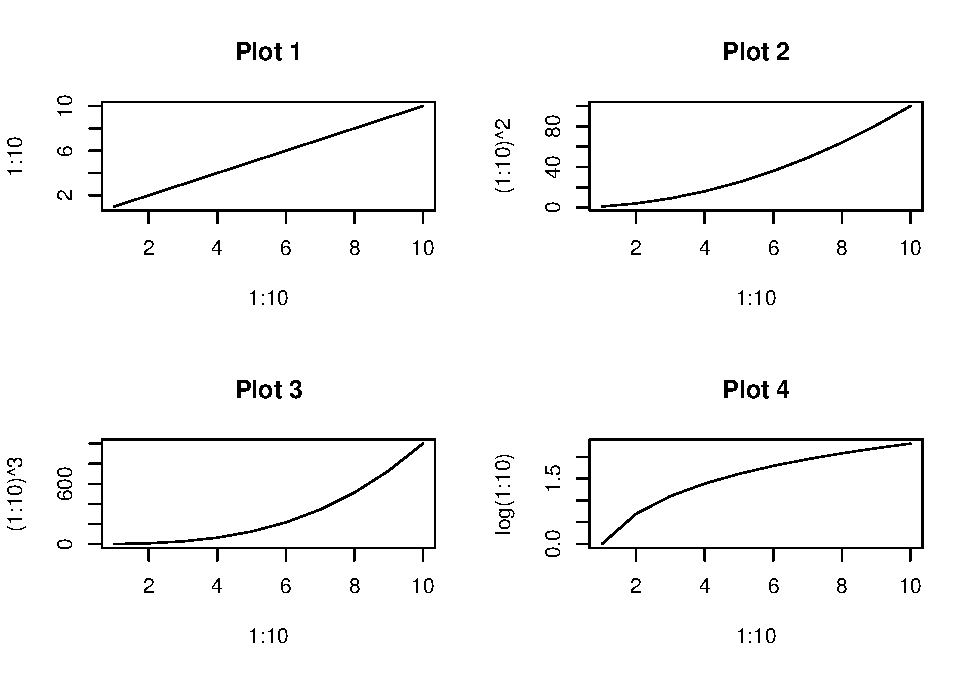
\includegraphics{_main_files/figure-latex/unnamed-chunk-47-1.pdf}

\textbf{ii). Customizing Plots with Grid Lines, Background Color, and Themes:}

\textbf{Grid Lines:} Use \textbf{grid()} function to add grid lines to the plot.

\textbf{Background Color:} Use \textbf{par(bg = ``color'')} to set background color for the plot.

\textbf{Themes:} Use themes from packages like ggplot2 to change the overall appearance of the plot. This will be covered under ggplot2 package chapter.

\textbf{Example with Grid Lines and Background Color:}

\begin{Shaded}
\begin{Highlighting}[]
\CommentTok{\# Example with grid lines and background color}
\FunctionTok{plot}\NormalTok{(}\DecValTok{1}\SpecialCharTok{:}\DecValTok{10}\NormalTok{, }\DecValTok{1}\SpecialCharTok{:}\DecValTok{10}\NormalTok{, }\AttributeTok{main =} \StringTok{"A Customized Simple Line Plot"}\NormalTok{, }\AttributeTok{type =} \StringTok{"l"}\NormalTok{, }\AttributeTok{xlab=}\StringTok{\textquotesingle{}Height\textquotesingle{}}\NormalTok{,}\AttributeTok{ylab =} \StringTok{\textquotesingle{}Weight\textquotesingle{}}\NormalTok{)}
\FunctionTok{grid}\NormalTok{() }\CommentTok{\# Add grid lines}
\end{Highlighting}
\end{Shaded}

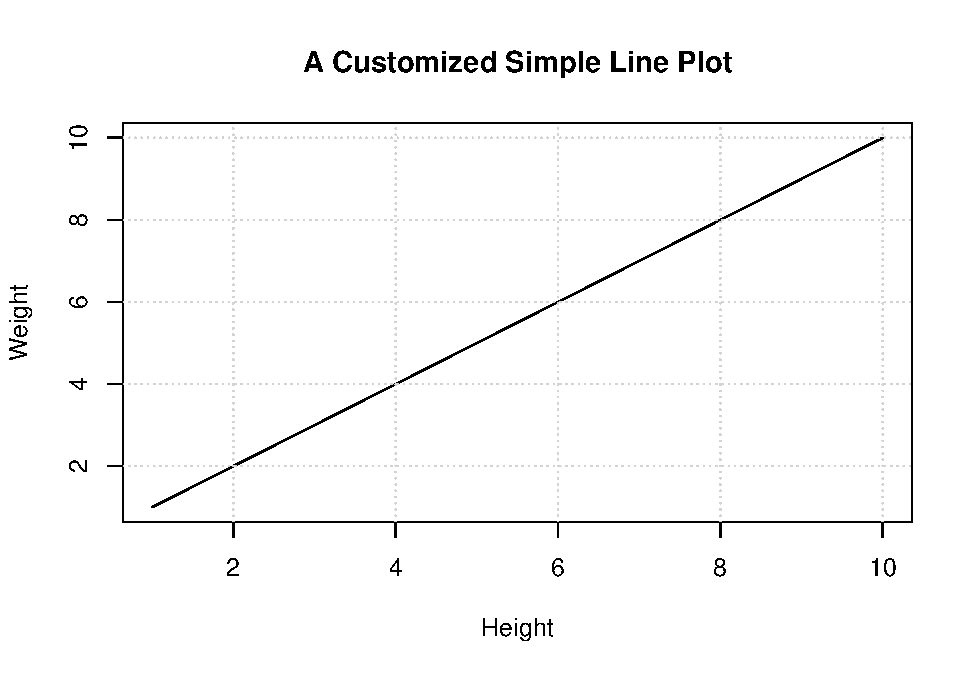
\includegraphics{_main_files/figure-latex/unnamed-chunk-48-1.pdf}

\begin{Shaded}
\begin{Highlighting}[]
\FunctionTok{par}\NormalTok{(}\AttributeTok{bg =} \StringTok{"lightblue"}\NormalTok{) }\CommentTok{\# Set background color}
\end{Highlighting}
\end{Shaded}

\section{Practical Examples: Exercise}\label{practical-examples-exercise}

\textbf{Exercise 11}

Read the \textbf{cabbages} dataset from \textbf{MASS} package. Remove the duplicated values of \textbf{``HeadWt''} and arrange the dataframe in descending order by \textbf{``HeadWt''} column. Plot a line plot of \textbf{``HeadWt''} against its square and apply blue color with the first line type. Add a second line plot of the square of cube of \textbf{``HeadWt''} , apply the red color and the line type should be the second one. Add a legend to the plot and position it at the top - left position with the names ``Square of Head Weight'' and ``Cube of Head Weight'' respectively. Maintain the same line types and colors that were used to plot. Add a title, `Comparison of Cabbage Trends'. Label the x-axis as `Head Weight' and y-axis should be blank

\begin{Shaded}
\begin{Highlighting}[]
\CommentTok{\# Your code}

\CommentTok{\# Solution}
\FunctionTok{library}\NormalTok{(dplyr)}
\FunctionTok{library}\NormalTok{(MASS)}

\NormalTok{cabbages }\OtherTok{\textless{}{-}}\NormalTok{ cabbages }\SpecialCharTok{\%\textgreater{}\%} 
  \FunctionTok{distinct}\NormalTok{(HeadWt, }\AttributeTok{.keep\_all =} \ConstantTok{TRUE}\NormalTok{) }\SpecialCharTok{\%\textgreater{}\%} 
  \FunctionTok{arrange}\NormalTok{(}\FunctionTok{desc}\NormalTok{(HeadWt),}\ConstantTok{FALSE}\NormalTok{)}

\FunctionTok{plot}\NormalTok{(cabbages}\SpecialCharTok{$}\NormalTok{HeadWt,(cabbages}\SpecialCharTok{$}\NormalTok{HeadWt)}\SpecialCharTok{\^{}}\DecValTok{2}\NormalTok{,}\AttributeTok{type =} \StringTok{\textquotesingle{}l\textquotesingle{}}\NormalTok{, }\AttributeTok{col=}\StringTok{\textquotesingle{}blue\textquotesingle{}}\NormalTok{, }
     \AttributeTok{lty=}\DecValTok{1}\NormalTok{,}\AttributeTok{main =} \StringTok{"Comparison of Unique Cabbage Trends"}\NormalTok{, }\AttributeTok{xlab =} \StringTok{"Head Weight"}\NormalTok{, }\AttributeTok{ylab =} \StringTok{""}\NormalTok{)}
\FunctionTok{lines}\NormalTok{(cabbages}\SpecialCharTok{$}\NormalTok{HeadWt,(cabbages}\SpecialCharTok{$}\NormalTok{HeadWt)}\SpecialCharTok{\^{}}\DecValTok{3}\NormalTok{,}\AttributeTok{type =} \StringTok{\textquotesingle{}l\textquotesingle{}}\NormalTok{, }\AttributeTok{col=}\StringTok{\textquotesingle{}red\textquotesingle{}}\NormalTok{, }\AttributeTok{lty=}\DecValTok{2}\NormalTok{)}
\FunctionTok{legend}\NormalTok{(}\StringTok{"topleft"}\NormalTok{, }\AttributeTok{legend =} \FunctionTok{c}\NormalTok{(}\StringTok{"Square of Head Weight"}\NormalTok{, }\StringTok{"Cube of Head Weight "}\NormalTok{), }\AttributeTok{col =} \FunctionTok{c}\NormalTok{(}\StringTok{"blue"}\NormalTok{, }\StringTok{"red"}\NormalTok{), }\AttributeTok{lty =} \FunctionTok{c}\NormalTok{(}\DecValTok{1}\NormalTok{, }\DecValTok{2}\NormalTok{))}
\end{Highlighting}
\end{Shaded}

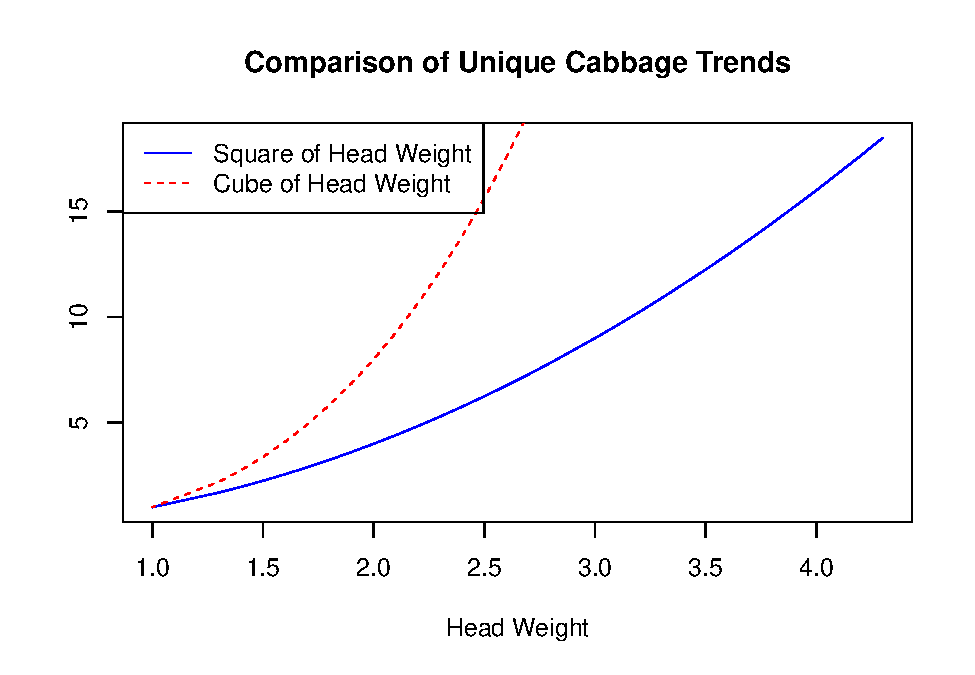
\includegraphics{_main_files/figure-latex/unnamed-chunk-49-1.pdf}

\textbf{Exercise 12 : Multiple Small Plots in One Graphic to Compare Different Data Sets}

Create a vector \textbf{x} of a sequence of numbers from 1 to 100. Create another vector \textbf{y1} which is the square of \textbf{x}. Create another vector \textbf{y2} which is the double of \textbf{x}. Lastly, create the last vector \textbf{y3} which is equivalent to \textbf{x} raised to the power of 1.5. Create three multiple small line plots and organize them in one row with three columns. All plots will use the same independent variable in the x-axis, i.e \textbf{x}.

\begin{enumerate}
\def\labelenumi{\roman{enumi})}
\tightlist
\item
  Plot x against y1. Give it the title,`Trend 1', x-axis should be labelled as `X' while y-axis=`Y' and color is blue.
\item
  Plot x against y2. Give it the title,`Trend 2', x-axis should be labelled as `X' while y-axis=`Y2',col is red.
\item
  Plot x against y3. Give it the title,`Trend 3', x-axis should be labelled as `X' while y-axis=`Y3',col is green.
\end{enumerate}

\begin{Shaded}
\begin{Highlighting}[]
\CommentTok{\# Your  data}

\CommentTok{\#Solution}
\CommentTok{\#Create data}
\NormalTok{x }\OtherTok{\textless{}{-}} \DecValTok{1}\SpecialCharTok{:}\DecValTok{100}
\NormalTok{y1 }\OtherTok{\textless{}{-}}\NormalTok{ x}\SpecialCharTok{\^{}}\DecValTok{2}
\NormalTok{y2 }\OtherTok{\textless{}{-}} \DecValTok{2} \SpecialCharTok{*}\NormalTok{ x}
\NormalTok{y3 }\OtherTok{\textless{}{-}}\NormalTok{ x}\SpecialCharTok{\^{}}\FloatTok{1.5}

\CommentTok{\# Create multiple small plots}
\FunctionTok{par}\NormalTok{(}\AttributeTok{mfrow =} \FunctionTok{c}\NormalTok{(}\DecValTok{1}\NormalTok{, }\DecValTok{3}\NormalTok{)) }\CommentTok{\# 1 row, 3 columns}

\CommentTok{\# Plot 1}
\FunctionTok{plot}\NormalTok{(x, y1, }\AttributeTok{type =} \StringTok{"l"}\NormalTok{, }\AttributeTok{col =} \StringTok{"blue"}\NormalTok{, }\AttributeTok{main =} \StringTok{"Trend 1"}\NormalTok{, }\AttributeTok{xlab =} \StringTok{"X"}\NormalTok{, }\AttributeTok{ylab =} \StringTok{"Y"}\NormalTok{)}

\CommentTok{\# Plot 2}
\FunctionTok{plot}\NormalTok{(x, y2, }\AttributeTok{type =} \StringTok{"l"}\NormalTok{, }\AttributeTok{col =} \StringTok{"red"}\NormalTok{, }\AttributeTok{main =} \StringTok{"Trend 2"}\NormalTok{, }\AttributeTok{xlab =} \StringTok{"X"}\NormalTok{, }\AttributeTok{ylab =} \StringTok{"Y2"}\NormalTok{)}

\CommentTok{\# Plot 3}
\FunctionTok{plot}\NormalTok{(x, y3, }\AttributeTok{type =} \StringTok{"l"}\NormalTok{, }\AttributeTok{col =} \StringTok{"green"}\NormalTok{, }\AttributeTok{main =} \StringTok{"Trend 3"}\NormalTok{, }\AttributeTok{xlab =} \StringTok{"X"}\NormalTok{, }\AttributeTok{ylab =} \StringTok{"Y3"}\NormalTok{)}
\end{Highlighting}
\end{Shaded}

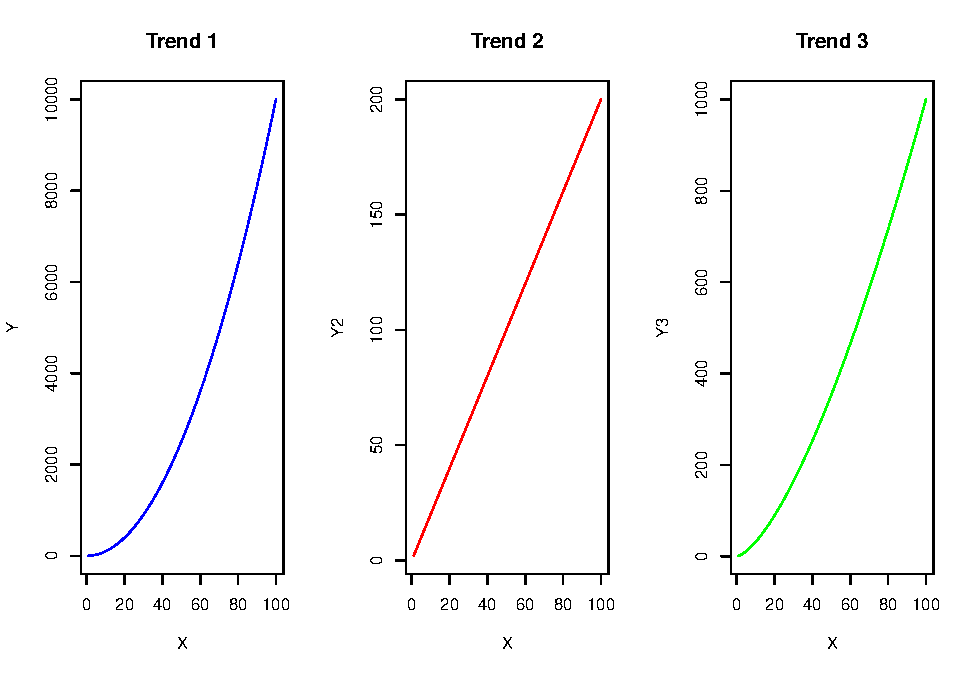
\includegraphics{_main_files/figure-latex/unnamed-chunk-50-1.pdf}

\begin{enumerate}
\def\labelenumi{\roman{enumi})}
\setcounter{enumi}{3}
\tightlist
\item
  Repeat the above similar plots but arranged in three rows and one column using \textbf{mfcol()}.
\end{enumerate}

\begin{Shaded}
\begin{Highlighting}[]
\CommentTok{\# Your  data}

\CommentTok{\#Solution}
\CommentTok{\#Create data}
\NormalTok{x }\OtherTok{\textless{}{-}} \DecValTok{1}\SpecialCharTok{:}\DecValTok{100}
\NormalTok{y1 }\OtherTok{\textless{}{-}}\NormalTok{ x}\SpecialCharTok{\^{}}\DecValTok{2}
\NormalTok{y2 }\OtherTok{\textless{}{-}} \DecValTok{2} \SpecialCharTok{*}\NormalTok{ x}
\NormalTok{y3 }\OtherTok{\textless{}{-}}\NormalTok{ x}\SpecialCharTok{\^{}}\FloatTok{1.5}

\CommentTok{\# Create multiple small plots}
\FunctionTok{par}\NormalTok{(}\AttributeTok{mfcol =} \FunctionTok{c}\NormalTok{(}\DecValTok{3}\NormalTok{, }\DecValTok{1}\NormalTok{)) }\CommentTok{\# 3 rows, 1 column}

\CommentTok{\# Plot 1}
\FunctionTok{plot}\NormalTok{(x, y1, }\AttributeTok{type =} \StringTok{"l"}\NormalTok{, }\AttributeTok{col =} \StringTok{"blue"}\NormalTok{, }\AttributeTok{main =} \StringTok{"Trend 1"}\NormalTok{, }\AttributeTok{xlab =} \StringTok{"X"}\NormalTok{, }\AttributeTok{ylab =} \StringTok{"Y"}\NormalTok{)}

\CommentTok{\# Plot 2}
\FunctionTok{plot}\NormalTok{(x, y2, }\AttributeTok{type =} \StringTok{"l"}\NormalTok{, }\AttributeTok{col =} \StringTok{"red"}\NormalTok{, }\AttributeTok{main =} \StringTok{"Trend 2"}\NormalTok{, }\AttributeTok{xlab =} \StringTok{"X"}\NormalTok{, }\AttributeTok{ylab =} \StringTok{"Y2"}\NormalTok{)}

\CommentTok{\# Plot 3}
\FunctionTok{plot}\NormalTok{(x, y3, }\AttributeTok{type =} \StringTok{"l"}\NormalTok{, }\AttributeTok{col =} \StringTok{"green"}\NormalTok{, }\AttributeTok{main =} \StringTok{"Trend 3"}\NormalTok{, }\AttributeTok{xlab =} \StringTok{"X"}\NormalTok{, }\AttributeTok{ylab =} \StringTok{"Y3"}\NormalTok{)}
\end{Highlighting}
\end{Shaded}

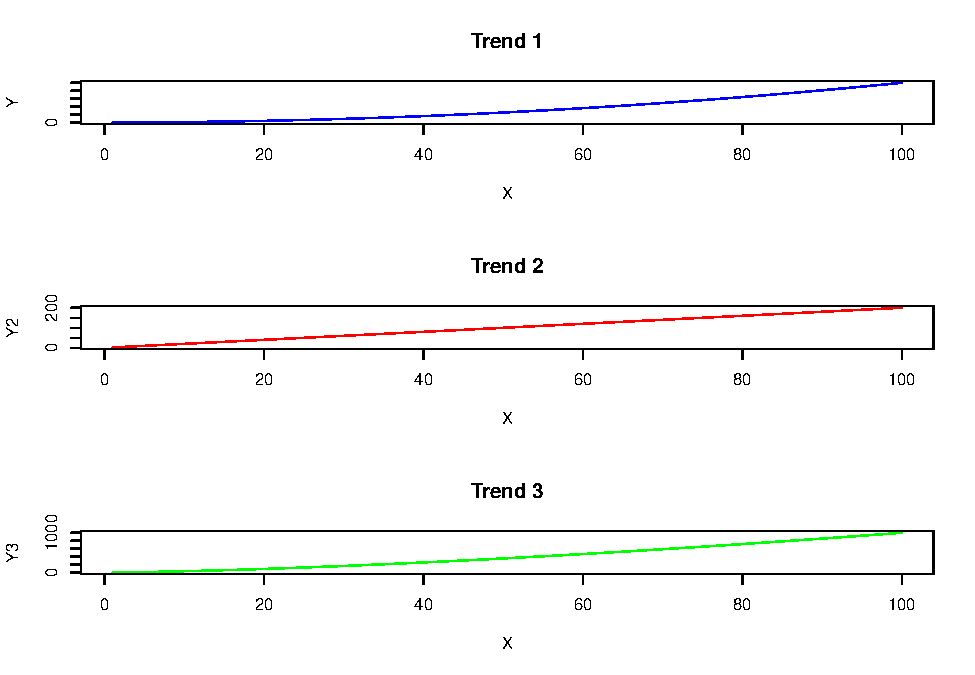
\includegraphics{_main_files/figure-latex/unnamed-chunk-51-1.pdf}

\chapter{ADVANCED BASE PLOTTING TECHNIQUES}\label{advanced-base-plotting-techniques}

\section{Combining Different Graph Types}\label{combining-different-graph-types}

We can overlay different types of plots, such as combining bar charts with line graphs, in R. Here's how this can be done along with customizing axes and scales:

\subsection{Overlay different types of plots}\label{overlay-different-types-of-plots}

\begin{Shaded}
\begin{Highlighting}[]
\CommentTok{\# Sample data}
\NormalTok{x }\OtherTok{\textless{}{-}} \DecValTok{1}\SpecialCharTok{:}\DecValTok{10}
\NormalTok{y1 }\OtherTok{\textless{}{-}}\NormalTok{ x}\SpecialCharTok{\^{}}\DecValTok{2}
\NormalTok{y2 }\OtherTok{\textless{}{-}} \DecValTok{2} \SpecialCharTok{*}\NormalTok{ x}
\NormalTok{y3 }\OtherTok{\textless{}{-}}\NormalTok{ x}\SpecialCharTok{\^{}}\FloatTok{1.5}

\CommentTok{\# Create a line plot}
\FunctionTok{plot}\NormalTok{(x, y1, }\AttributeTok{type =} \StringTok{"l"}\NormalTok{, }\AttributeTok{col =} \StringTok{"blue"}\NormalTok{, }\AttributeTok{main =} \StringTok{"Combining Different Graph Types"}\NormalTok{, }\AttributeTok{xlab =} \StringTok{"X"}\NormalTok{, }\AttributeTok{ylab =} \StringTok{"Y"}\NormalTok{)}

\CommentTok{\# Add points to the line plot}
\FunctionTok{points}\NormalTok{(x, y1, }\AttributeTok{col =} \StringTok{"blue"}\NormalTok{, }\AttributeTok{pch =} \DecValTok{16}\NormalTok{)}

\CommentTok{\# Add a bar plot}
\FunctionTok{barplot}\NormalTok{(y2, }\AttributeTok{col =} \StringTok{"red"}\NormalTok{, }\AttributeTok{add =} \ConstantTok{TRUE}\NormalTok{)}

\CommentTok{\# Add a second line plot}
\FunctionTok{lines}\NormalTok{(x, y3, }\AttributeTok{col =} \StringTok{"green"}\NormalTok{)}

\CommentTok{\# Add a legend}
\FunctionTok{legend}\NormalTok{(}\StringTok{"topleft"}\NormalTok{, }\AttributeTok{legend =} \FunctionTok{c}\NormalTok{(}\StringTok{"Trend 1"}\NormalTok{, }\StringTok{"Trend 2"}\NormalTok{, }\StringTok{"Trend 3"}\NormalTok{), }\AttributeTok{col =} \FunctionTok{c}\NormalTok{(}\StringTok{"blue"}\NormalTok{, }\StringTok{"red"}\NormalTok{, }\StringTok{"green"}\NormalTok{), }\AttributeTok{lty =} \FunctionTok{c}\NormalTok{(}\DecValTok{1}\NormalTok{, }\ConstantTok{NA}\NormalTok{, }\DecValTok{1}\NormalTok{), }\AttributeTok{pch =} \FunctionTok{c}\NormalTok{(}\DecValTok{16}\NormalTok{, }\ConstantTok{NA}\NormalTok{, }\ConstantTok{NA}\NormalTok{))}
\end{Highlighting}
\end{Shaded}

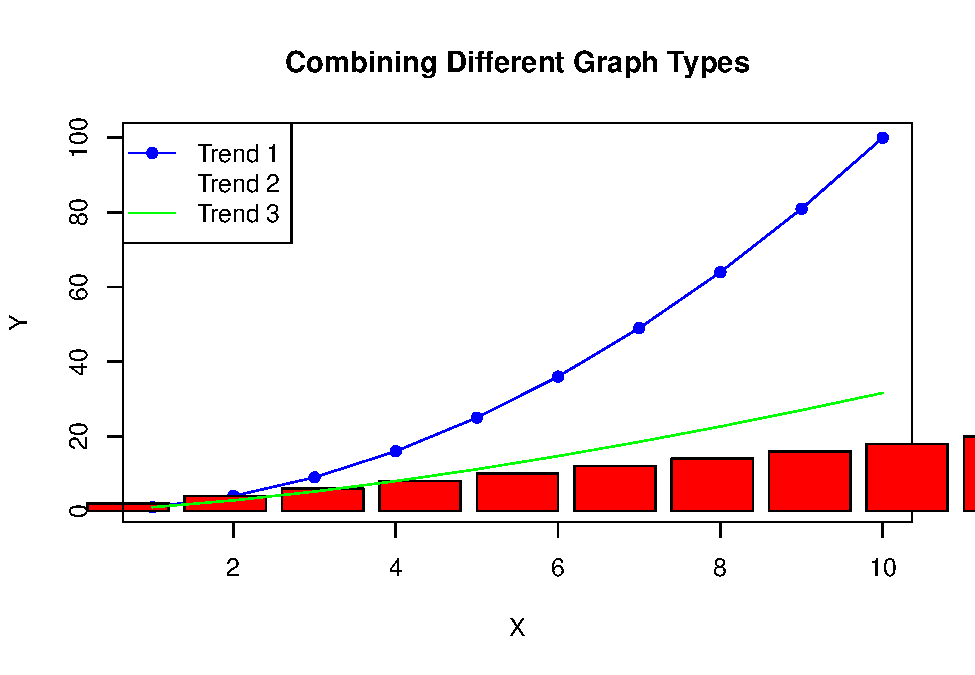
\includegraphics{_main_files/figure-latex/unnamed-chunk-53-1.pdf}

\subsection{Axes and scales customization to accomodate combined plots}\label{axes-and-scales-customization-to-accomodate-combined-plots}

\begin{Shaded}
\begin{Highlighting}[]
\CommentTok{\# Set custom axis limits}
\FunctionTok{plot}\NormalTok{(x, y1, }\AttributeTok{type =} \StringTok{"l"}\NormalTok{, }\AttributeTok{col =} \StringTok{"blue"}\NormalTok{, }\AttributeTok{main =} \StringTok{"Combining Different Graph Types"}\NormalTok{, }\AttributeTok{xlab =} \StringTok{"X"}\NormalTok{, }\AttributeTok{ylab =} \StringTok{"Y"}\NormalTok{, }\AttributeTok{ylim =} \FunctionTok{c}\NormalTok{(}\DecValTok{0}\NormalTok{, }\FunctionTok{max}\NormalTok{(y1, y2, y3)))}

\CommentTok{\# Add points to the line plot}
\FunctionTok{points}\NormalTok{(x, y1, }\AttributeTok{col =} \StringTok{"blue"}\NormalTok{, }\AttributeTok{pch =} \DecValTok{16}\NormalTok{)}

\CommentTok{\# Add a bar plot}
\FunctionTok{barplot}\NormalTok{(y2, }\AttributeTok{col =} \StringTok{"red"}\NormalTok{, }\AttributeTok{add =} \ConstantTok{TRUE}\NormalTok{, }\AttributeTok{ylim =} \FunctionTok{c}\NormalTok{(}\DecValTok{0}\NormalTok{, }\FunctionTok{max}\NormalTok{(y1, y2, y3)))}

\CommentTok{\# Add a second line plot}
\FunctionTok{lines}\NormalTok{(x, y3, }\AttributeTok{col =} \StringTok{"green"}\NormalTok{)}

\CommentTok{\# Add a legend}
\FunctionTok{legend}\NormalTok{(}\StringTok{"topleft"}\NormalTok{, }\AttributeTok{legend =} \FunctionTok{c}\NormalTok{(}\StringTok{"Trend 1"}\NormalTok{, }\StringTok{"Trend 2"}\NormalTok{, }\StringTok{"Trend 3"}\NormalTok{), }\AttributeTok{col =} \FunctionTok{c}\NormalTok{(}\StringTok{"blue"}\NormalTok{, }\StringTok{"red"}\NormalTok{, }\StringTok{"green"}\NormalTok{), }\AttributeTok{lty =} \FunctionTok{c}\NormalTok{(}\DecValTok{1}\NormalTok{, }\ConstantTok{NA}\NormalTok{, }\DecValTok{1}\NormalTok{), }\AttributeTok{pch =} \FunctionTok{c}\NormalTok{(}\DecValTok{16}\NormalTok{, }\ConstantTok{NA}\NormalTok{, }\ConstantTok{NA}\NormalTok{))}
\end{Highlighting}
\end{Shaded}

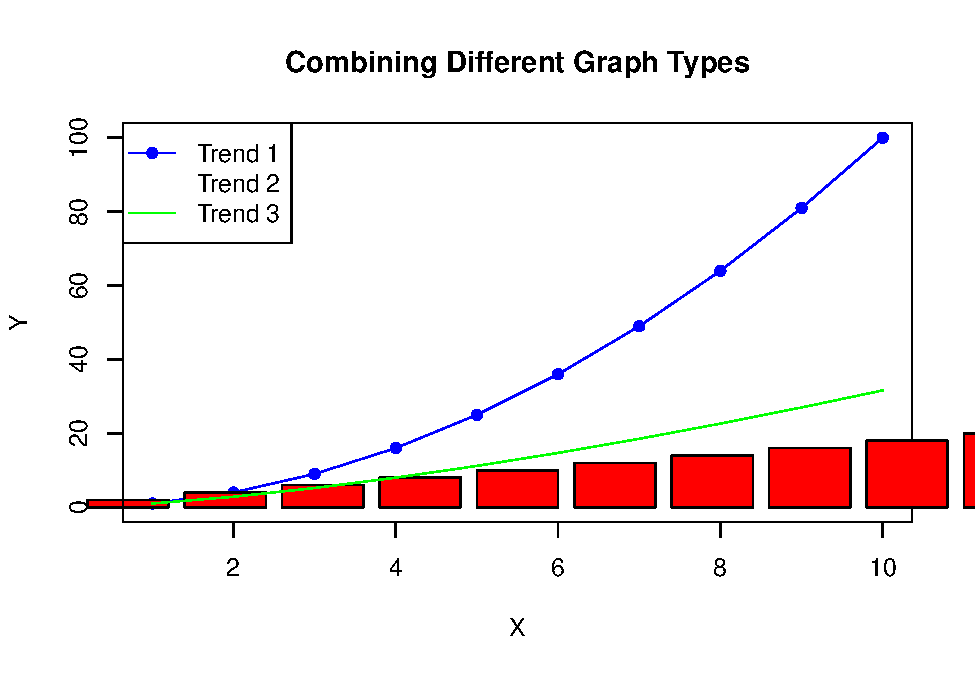
\includegraphics{_main_files/figure-latex/unnamed-chunk-54-1.pdf}

\section{Interactive Graphics in Base R}\label{interactive-graphics-in-base-r}

\subsection{Introduction to using the locator() function for interactive plotting}\label{introduction-to-using-the-locator-function-for-interactive-plotting}

Base R provides basic functionality for creating interactive plots using the locator() function. Here's how you can use locator() for interactive plotting and create dynamic plots that respond to user input or updates in data:

\begin{Shaded}
\begin{Highlighting}[]
\CommentTok{\# Sample data}
\NormalTok{x }\OtherTok{\textless{}{-}} \DecValTok{1}\SpecialCharTok{:}\DecValTok{10}
\NormalTok{y }\OtherTok{\textless{}{-}}\NormalTok{ x}\SpecialCharTok{\^{}}\DecValTok{2}

\CommentTok{\# Plot data}
\FunctionTok{plot}\NormalTok{(x, y, }\AttributeTok{type =} \StringTok{"l"}\NormalTok{, }\AttributeTok{main =} \StringTok{"Interactive Plotting with locator()"}\NormalTok{)}

\CommentTok{\# Add points interactively}
\FunctionTok{points}\NormalTok{(}\FunctionTok{locator}\NormalTok{(}\DecValTok{5}\NormalTok{), }\AttributeTok{col =} \StringTok{"red"}\NormalTok{, }\AttributeTok{pch =} \DecValTok{16}\NormalTok{)}
\end{Highlighting}
\end{Shaded}

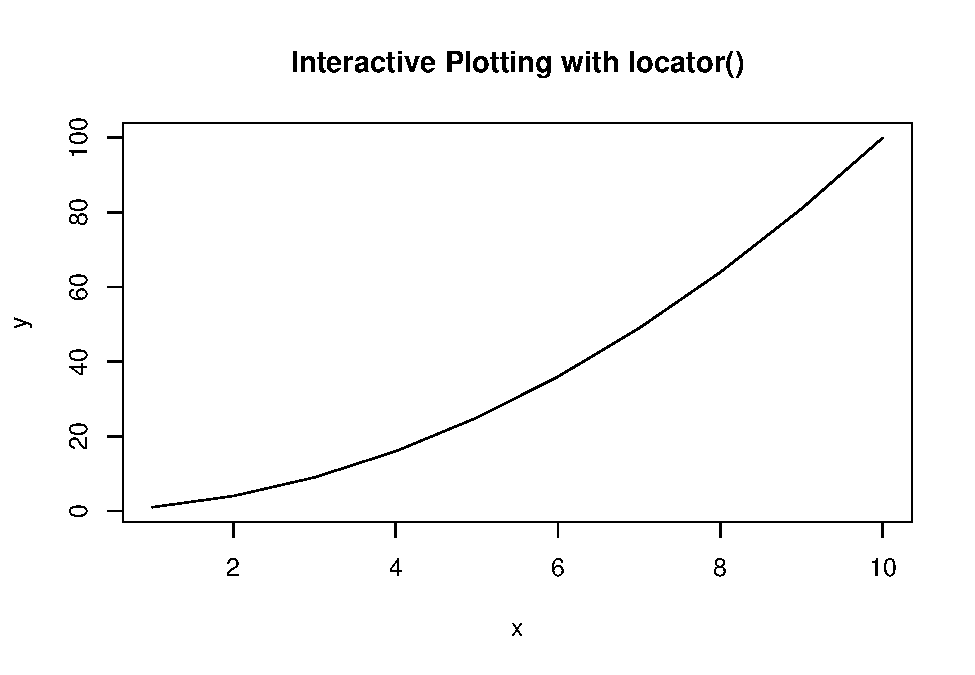
\includegraphics{_main_files/figure-latex/unnamed-chunk-55-1.pdf}

\subsection{Creating dynamic plots that respond to user input or updates in data}\label{creating-dynamic-plots-that-respond-to-user-input-or-updates-in-data}

\begin{Shaded}
\begin{Highlighting}[]
\CommentTok{\# Dynamic plot that responds to user input}
\NormalTok{plot\_dynamic }\OtherTok{\textless{}{-}} \ControlFlowTok{function}\NormalTok{() \{}
  \CommentTok{\# Sample data}
\NormalTok{  x }\OtherTok{\textless{}{-}} \DecValTok{1}\SpecialCharTok{:}\DecValTok{10}
\NormalTok{  y }\OtherTok{\textless{}{-}}\NormalTok{ x}\SpecialCharTok{\^{}}\DecValTok{2}
  
  \CommentTok{\# Plot data}
  \FunctionTok{plot}\NormalTok{(x, y, }\AttributeTok{type =} \StringTok{"l"}\NormalTok{, }\AttributeTok{main =} \StringTok{"Dynamic Plot with User Input"}\NormalTok{)}
  
  \CommentTok{\# Add points interactively}
  \FunctionTok{points}\NormalTok{(}\FunctionTok{locator}\NormalTok{(}\DecValTok{5}\NormalTok{), }\AttributeTok{col =} \StringTok{"red"}\NormalTok{, }\AttributeTok{pch =} \DecValTok{16}\NormalTok{)}
\NormalTok{\}}

\CommentTok{\# Call the function to create dynamic plot}
\FunctionTok{plot\_dynamic}\NormalTok{()}
\end{Highlighting}
\end{Shaded}

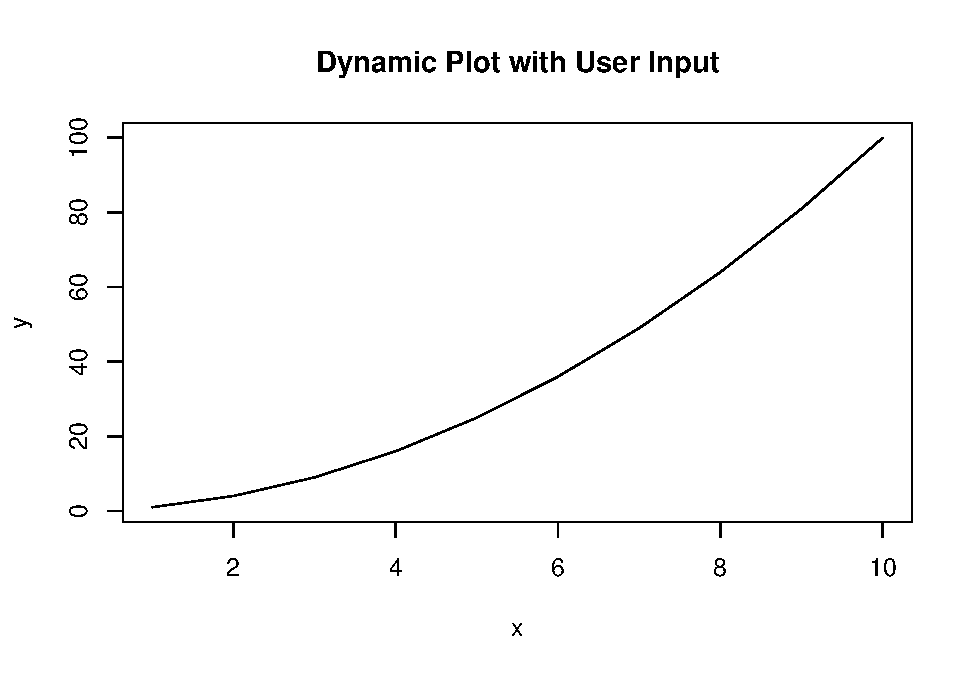
\includegraphics{_main_files/figure-latex/unnamed-chunk-56-1.pdf}

\chapter{PLOTTING TIME SERIES DATA}\label{plotting-time-series-data}

\section{Introduction}\label{introduction-3}

The plotting of time series object is most likely one of the steps of the analysis of time-series data. The two main objectives of this chapter are:

\begin{itemize}
\tightlist
\item
  Understand specific considerations for plotting time series data in R.
\item
  Learn to effectively visualize time-dependent data using R's base graphics.
\end{itemize}

\subsection{Importance of time series analysis in various fields like finance, meteorology, and epidemiology}\label{importance-of-time-series-analysis-in-various-fields-like-finance-meteorology-and-epidemiology}

Time series analysis plays a crucial role in various fields such as finance, meteorology, epidemiology, and many others. Understanding time series data and effectively visualizing it are essential for extracting meaningful insights. In this chapter, we will explore the importance of time series analysis and the challenges associated with visualizing time series data.

Time series analysis is vital in various fields including:

\begin{itemize}
\item
  \textbf{Finance:} Analyzing stock prices, market trends, and forecasting.
\item
  \textbf{Meteorology:} Studying weather patterns, climate change, and forecasting.
\item
  \textbf{Epidemiology:} Tracking disease outbreaks, analyzing trends, and forecasting.
\end{itemize}

\subsection{Basic concepts related to time series data and its visualization challenges.}\label{basic-concepts-related-to-time-series-data-and-its-visualization-challenges.}

\begin{itemize}
\item
  \textbf{Time Series Data:} Time series data consists of observations or measurements taken at different points in time.
\item
  \textbf{Temporal Patterns:} Time series data often exhibits various temporal patterns such as trend, seasonality, and cycles.
\item
  \textbf{Visualization Challenges:} Visualizing time series data poses challenges due to its temporal nature and the need to effectively represent temporal patterns.
\end{itemize}

\section{Time Series Data Basics}\label{time-series-data-basics}

Time series data in R is commonly represented using the \textbf{ts} class. The time series object must have a \textbf{Date} or \textbf{POSIXct/lt} column and at least one numeric column.

\subsection{Introduction to time series objects in R (ts class).}\label{introduction-to-time-series-objects-in-r-ts-class.}

\begin{itemize}
\item
  The \textbf{ts} class in R is a basic time series object.
\item
  It is suitable for regularly spaced time series data.
\item
  Time series objects are created using the \textbf{ts()} function.
\end{itemize}

\textbf{Example: Creating a time series object}

\begin{Shaded}
\begin{Highlighting}[]
\CommentTok{\# Sample time series data}
\NormalTok{data }\OtherTok{\textless{}{-}} \FunctionTok{c}\NormalTok{(}\DecValTok{10}\NormalTok{, }\DecValTok{15}\NormalTok{, }\DecValTok{20}\NormalTok{, }\DecValTok{25}\NormalTok{, }\DecValTok{30}\NormalTok{)}
\NormalTok{time\_series }\OtherTok{\textless{}{-}} \FunctionTok{ts}\NormalTok{(data)}

\CommentTok{\# View the time series object}
\FunctionTok{print}\NormalTok{(time\_series)}
\end{Highlighting}
\end{Shaded}

\begin{verbatim}
## Time Series:
## Start = 1 
## End = 5 
## Frequency = 1 
## [1] 10 15 20 25 30
\end{verbatim}

\subsection{How to convert standard date formats into time series objects}\label{how-to-convert-standard-date-formats-into-time-series-objects}

R provides several functions to convert standard date formats into time series objects, such as \textbf{as.ts()} and \textbf{ts()}.

\textbf{Example: Converting Standard Date Formats into Time Series Objects}

\begin{Shaded}
\begin{Highlighting}[]
\CommentTok{\# Sample data with dates}
\NormalTok{dates }\OtherTok{\textless{}{-}} \FunctionTok{as.Date}\NormalTok{(}\FunctionTok{c}\NormalTok{(}\StringTok{"2022{-}01{-}01"}\NormalTok{, }\StringTok{"2022{-}02{-}01"}\NormalTok{, }\StringTok{"2022{-}03{-}01"}\NormalTok{, }\StringTok{"2022{-}04{-}01"}\NormalTok{, }\StringTok{"2022{-}05{-}01"}\NormalTok{))}
\NormalTok{data }\OtherTok{\textless{}{-}} \FunctionTok{c}\NormalTok{(}\DecValTok{10}\NormalTok{, }\DecValTok{15}\NormalTok{, }\DecValTok{20}\NormalTok{, }\DecValTok{25}\NormalTok{, }\DecValTok{30}\NormalTok{)}

\CommentTok{\# Create a time series object}
\NormalTok{time\_series }\OtherTok{\textless{}{-}} \FunctionTok{ts}\NormalTok{(data, }\AttributeTok{start =} \FunctionTok{c}\NormalTok{(}\FunctionTok{as.POSIXlt}\NormalTok{(dates[}\DecValTok{1}\NormalTok{])}\SpecialCharTok{$}\NormalTok{year }\SpecialCharTok{+} \DecValTok{1900}\NormalTok{, }\FunctionTok{as.POSIXlt}\NormalTok{(dates[}\DecValTok{1}\NormalTok{])}\SpecialCharTok{$}\NormalTok{mon }\SpecialCharTok{+} \DecValTok{1}\NormalTok{), }\AttributeTok{frequency =} \DecValTok{12}\NormalTok{)}

\CommentTok{\# View the time series object}
\FunctionTok{print}\NormalTok{(time\_series)}
\end{Highlighting}
\end{Shaded}

\begin{verbatim}
##      Jan Feb Mar Apr May
## 2022  10  15  20  25  30
\end{verbatim}

In this example, \textbf{start} indicates the start of the time series, and \textbf{frequency} indicates the number of observations per unit of time. Here, \textbf{frequency = 12} indicates monthly data. These are the basics of working with time series data objects in R.

\section{Visualizing Time Series}\label{visualizing-time-series}

Let's load and plot the \textbf{USgas} series, a \textbf{ts} object which is attached in the TSstudio package:

\begin{Shaded}
\begin{Highlighting}[]
\FunctionTok{library}\NormalTok{(TSstudio)}
\end{Highlighting}
\end{Shaded}

\begin{verbatim}
## Warning: package 'TSstudio' was built under R version 4.3.3
\end{verbatim}

\begin{Shaded}
\begin{Highlighting}[]
\FunctionTok{data}\NormalTok{(USgas)}

\FunctionTok{ts\_info}\NormalTok{(USgas)}
\end{Highlighting}
\end{Shaded}

\begin{verbatim}
##  The USgas series is a ts object with 1 variable and 238 observations
##  Frequency: 12 
##  Start time: 2000 1 
##  End time: 2019 10
\end{verbatim}

\subsection{Creating line plots for time series data}\label{creating-line-plots-for-time-series-data}

Let us plot the \textbf{USgas} series using the base R \textbf{plot()} function.

\begin{Shaded}
\begin{Highlighting}[]
\FunctionTok{plot}\NormalTok{(USgas)}
\end{Highlighting}
\end{Shaded}

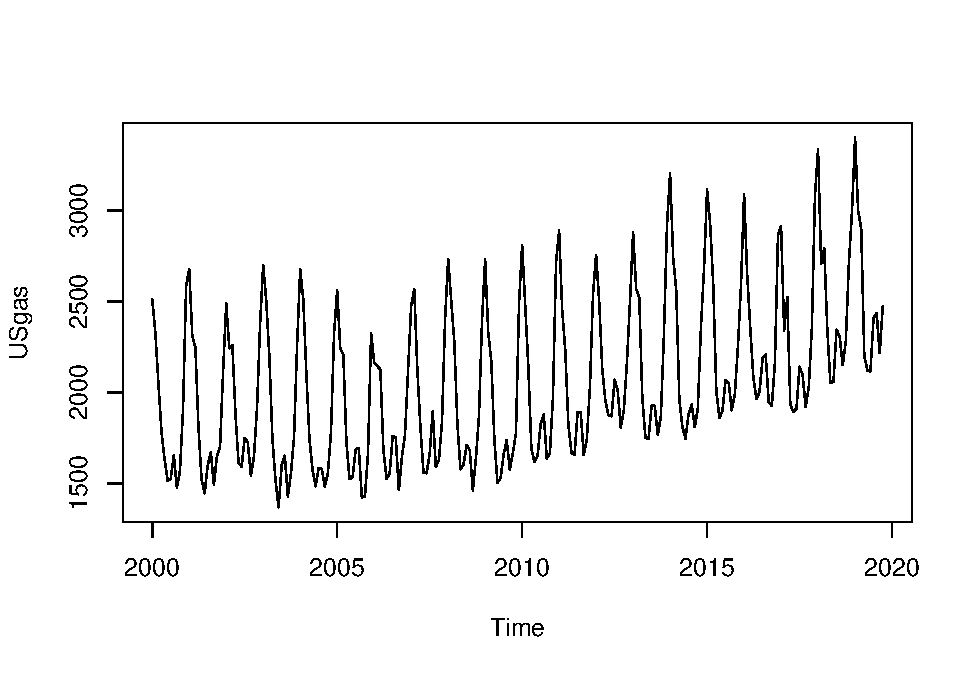
\includegraphics{_main_files/figure-latex/unnamed-chunk-61-1.pdf}

\subsection{Techniques for highlighting trends, seasonality, and anomalies}\label{techniques-for-highlighting-trends-seasonality-and-anomalies}

\begin{itemize}
\item
  \textbf{Trends:} Use \textbf{lines()} function to overlay a trend line on the plot.
\item
  \textbf{Seasonality:} Use \textbf{seasonplot()} function from the forecast package to visualize seasonal patterns.
\item
  \textbf{Anomalies:} Use \textbf{points()} function to mark anomalies on the plot.
\end{itemize}

\textbf{Example:} Let's visualize the \textbf{USgas} time series data and highlight trends, seasonality, and anomalies:

\begin{Shaded}
\begin{Highlighting}[]
\CommentTok{\# Install and load the necessary packages}
\CommentTok{\#install.packages("forecast")}
\FunctionTok{library}\NormalTok{(forecast)}

\CommentTok{\# Load the USgas time series object}
\FunctionTok{data}\NormalTok{(}\StringTok{"USgas"}\NormalTok{)}

\CommentTok{\# Convert the ts object into a data frame}
\NormalTok{USgas\_df }\OtherTok{\textless{}{-}} \FunctionTok{data.frame}\NormalTok{(}\AttributeTok{year =} \FunctionTok{time}\NormalTok{(USgas), }\AttributeTok{production =} \FunctionTok{as.numeric}\NormalTok{(USgas))}

\CommentTok{\# Apply loess function}
\NormalTok{trend }\OtherTok{\textless{}{-}} \FunctionTok{loess}\NormalTok{(production }\SpecialCharTok{\textasciitilde{}}\NormalTok{ year, }\AttributeTok{data =}\NormalTok{ USgas\_df)}

\CommentTok{\# Extract the trend values}
\NormalTok{trend\_values }\OtherTok{\textless{}{-}} \FunctionTok{predict}\NormalTok{(trend)}

\CommentTok{\# Plot the USgas time series}
\FunctionTok{plot}\NormalTok{(USgas, }\AttributeTok{main =} \StringTok{"US Gas Production Time Series"}\NormalTok{, }\AttributeTok{xlab =} \StringTok{"Year"}\NormalTok{, }\AttributeTok{ylab =} \StringTok{"Gas Production"}\NormalTok{)}
\end{Highlighting}
\end{Shaded}

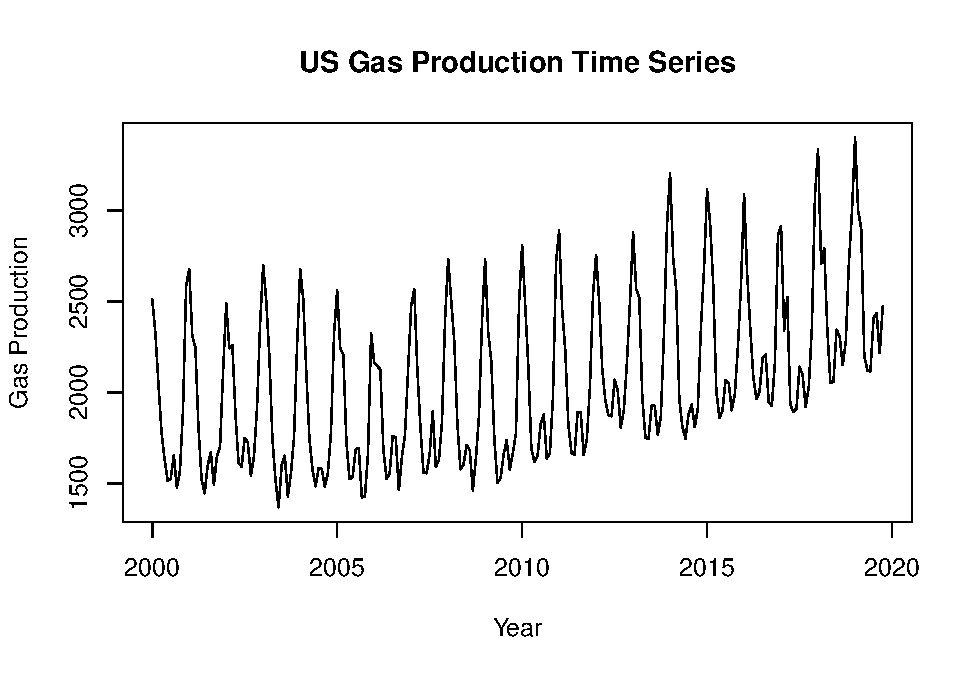
\includegraphics{_main_files/figure-latex/unnamed-chunk-62-1.pdf}

\begin{Shaded}
\begin{Highlighting}[]
\CommentTok{\# Add trend line}
\CommentTok{\#lines(time(USgas), trend\_values, col = "blue")}

\CommentTok{\# Visualize seasonal pattern}
\FunctionTok{seasonplot}\NormalTok{(USgas, }\AttributeTok{col =} \StringTok{"green"}\NormalTok{)}

\CommentTok{\# Identify anomalies}
\NormalTok{anomalies }\OtherTok{\textless{}{-}} \FunctionTok{which}\NormalTok{(USgas }\SpecialCharTok{\textgreater{}} \FunctionTok{mean}\NormalTok{(USgas) }\SpecialCharTok{+} \DecValTok{2} \SpecialCharTok{*} \FunctionTok{sd}\NormalTok{(USgas) }\SpecialCharTok{|}\NormalTok{ USgas }\SpecialCharTok{\textless{}} \FunctionTok{mean}\NormalTok{(USgas) }\SpecialCharTok{{-}} \DecValTok{2} \SpecialCharTok{*} \FunctionTok{sd}\NormalTok{(USgas))}
\FunctionTok{points}\NormalTok{(}\FunctionTok{time}\NormalTok{(USgas)[anomalies], USgas[anomalies], }\AttributeTok{col =} \StringTok{"red"}\NormalTok{, }\AttributeTok{pch =} \DecValTok{16}\NormalTok{)}
\end{Highlighting}
\end{Shaded}

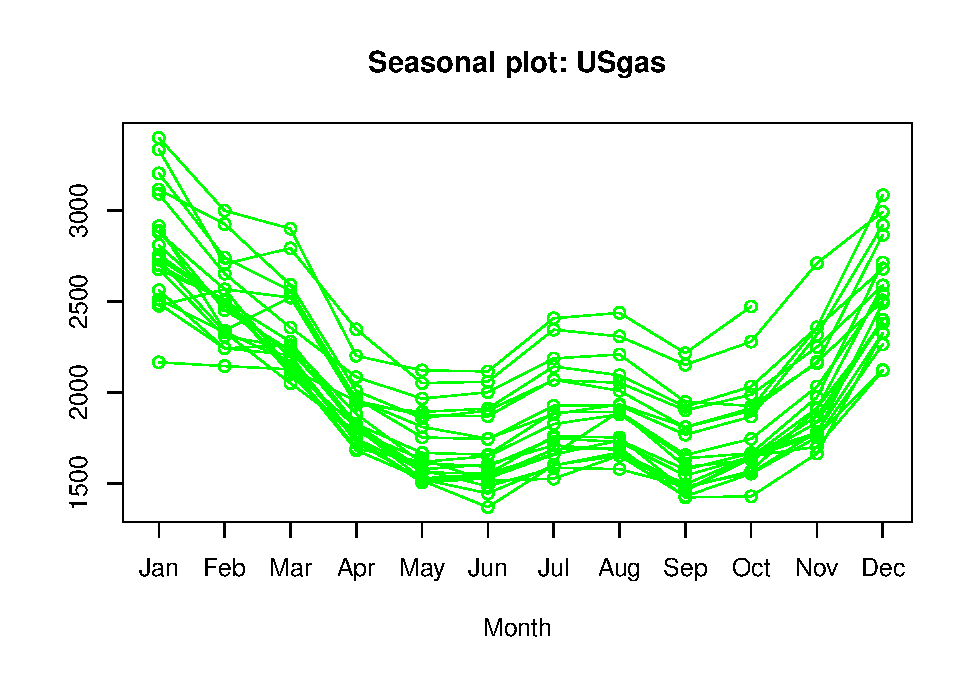
\includegraphics{_main_files/figure-latex/unnamed-chunk-62-2.pdf}

\section{Advanced Time Series Visualization}\label{advanced-time-series-visualization}

\subsection{\texorpdfstring{Advance customization using ts\_plot() function from \textbf{plotly} package}{Advance customization using ts\_plot() function from plotly package}}\label{advance-customization-using-ts_plot-function-from-plotly-package}

The \textbf{ts\_plot} is a wraper of the \textbf{plotly} package plotting functions for time series objects, therefore, the output of the \textbf{ts\_plot} is a \textbf{plotly} object. Advance customization of the \textbf{ts\_plot} output can be done with plotly's layout function. For example, let's re plot the \textbf{USgas} series and customize the background to black:

\begin{Shaded}
\begin{Highlighting}[]
\FunctionTok{library}\NormalTok{(plotly)}

\FunctionTok{ts\_plot}\NormalTok{(USgas,}
        \AttributeTok{title =} \StringTok{"US Monthly Natural Gas Consumption"}\NormalTok{,}
        \AttributeTok{Xtitle =} \StringTok{"Time"}\NormalTok{,}
        \AttributeTok{Ytitle =} \StringTok{"Billion Cubic Feet"}\NormalTok{,}
        \AttributeTok{color =}  \StringTok{"pink"}\NormalTok{,}
        \AttributeTok{Xgrid =} \ConstantTok{TRUE}\NormalTok{,}
        \AttributeTok{Ygrid =} \ConstantTok{TRUE}\NormalTok{) }\SpecialCharTok{\%\textgreater{}\%}
  \FunctionTok{layout}\NormalTok{(}\AttributeTok{paper\_bgcolor =} \StringTok{"black"}\NormalTok{,}
         \AttributeTok{plot\_bgcolor =} \StringTok{"black"}\NormalTok{,}
         \AttributeTok{font =} \FunctionTok{list}\NormalTok{(}\AttributeTok{color =} \StringTok{"white"}\NormalTok{),}
         \AttributeTok{yaxis =} \FunctionTok{list}\NormalTok{(}\AttributeTok{linecolor =} \StringTok{"\#6b6b6b"}\NormalTok{,}
                      \AttributeTok{zerolinecolor =} \StringTok{"\#6b6b6b"}\NormalTok{,}
                      \AttributeTok{gridcolor=} \StringTok{"\#444444"}\NormalTok{),}
         \AttributeTok{xaxis =} \FunctionTok{list}\NormalTok{(}\AttributeTok{linecolor =} \StringTok{"\#6b6b6b"}\NormalTok{,}
                      \AttributeTok{zerolinecolor =} \StringTok{"\#6b6b6b"}\NormalTok{,}
                      \AttributeTok{gridcolor=} \StringTok{"\#444444"}\NormalTok{))}
\end{Highlighting}
\end{Shaded}

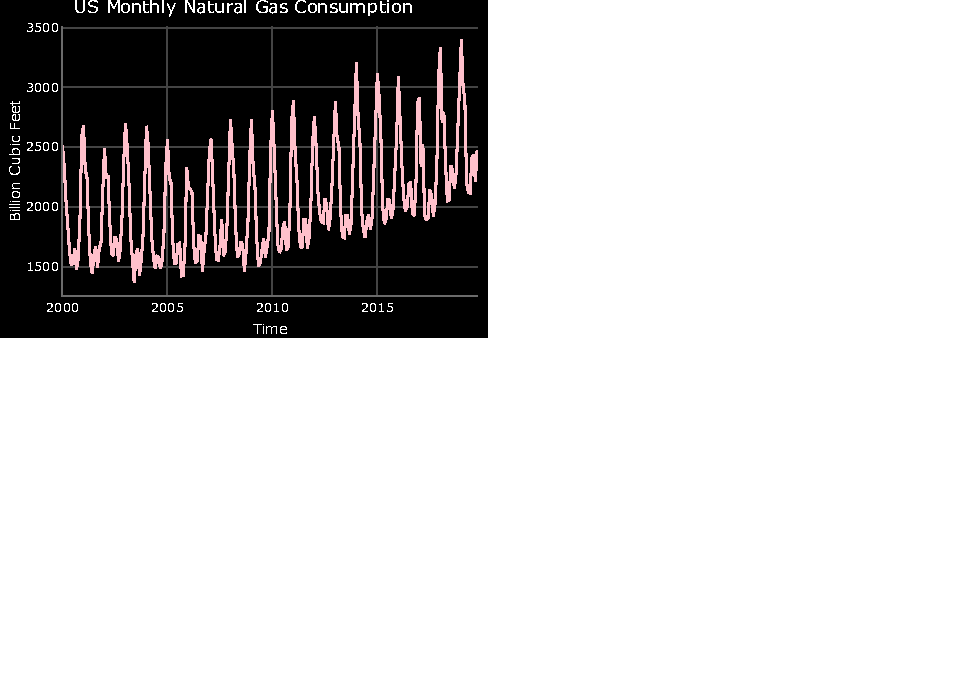
\includegraphics{_main_files/figure-latex/unnamed-chunk-63-1.pdf}

Note that the \textbf{Xgrid} and \textbf{Ygrid} arguments, when set to \textbf{TRUE}, add the corresponding X and Y grid lines.

\subsection{Plotting multiple time series on a single graph for comparative analysis}\label{plotting-multiple-time-series-on-a-single-graph-for-comparative-analysis}

The plotting of a multiple time series object is straightforward. Let's load the \textbf{Coffee\_Prices} an \textbf{mts} object that represents the monthly prices of the Robusta and Arabica coffee prices (USD per Kg.):

\begin{Shaded}
\begin{Highlighting}[]
\FunctionTok{data}\NormalTok{(}\StringTok{"Coffee\_Prices"}\NormalTok{)}

\FunctionTok{ts\_info}\NormalTok{(Coffee\_Prices)}
\end{Highlighting}
\end{Shaded}

\begin{verbatim}
##  The Coffee_Prices series is a mts object with 2 variables and 701 observations
##  Frequency: 12 
##  Start time: 1960 1 
##  End time: 2018 5
\end{verbatim}

\begin{Shaded}
\begin{Highlighting}[]
\FunctionTok{ts\_plot}\NormalTok{(Coffee\_Prices,}
        \AttributeTok{title =} \StringTok{"Comparison of Robusta and Arabica coffee prices"}\NormalTok{)}
\end{Highlighting}
\end{Shaded}

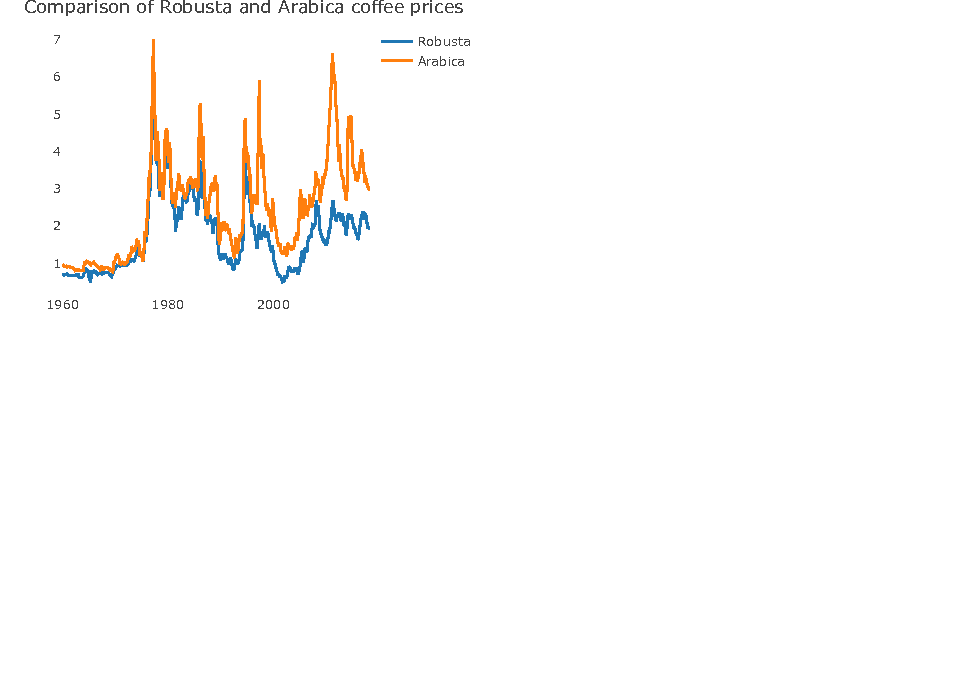
\includegraphics{_main_files/figure-latex/unnamed-chunk-64-1.pdf}

By default, the function will plot all the series in one plot. Plotting the different series on a separate plot can be done by setting the type argument to multiple:

\begin{Shaded}
\begin{Highlighting}[]
\FunctionTok{ts\_plot}\NormalTok{(Coffee\_Prices,}
        \AttributeTok{title =} \StringTok{"Comparison of Robusta and Arabica coffee prices"}\NormalTok{,}
        \AttributeTok{type =} \StringTok{"multiple"}\NormalTok{)}
\end{Highlighting}
\end{Shaded}

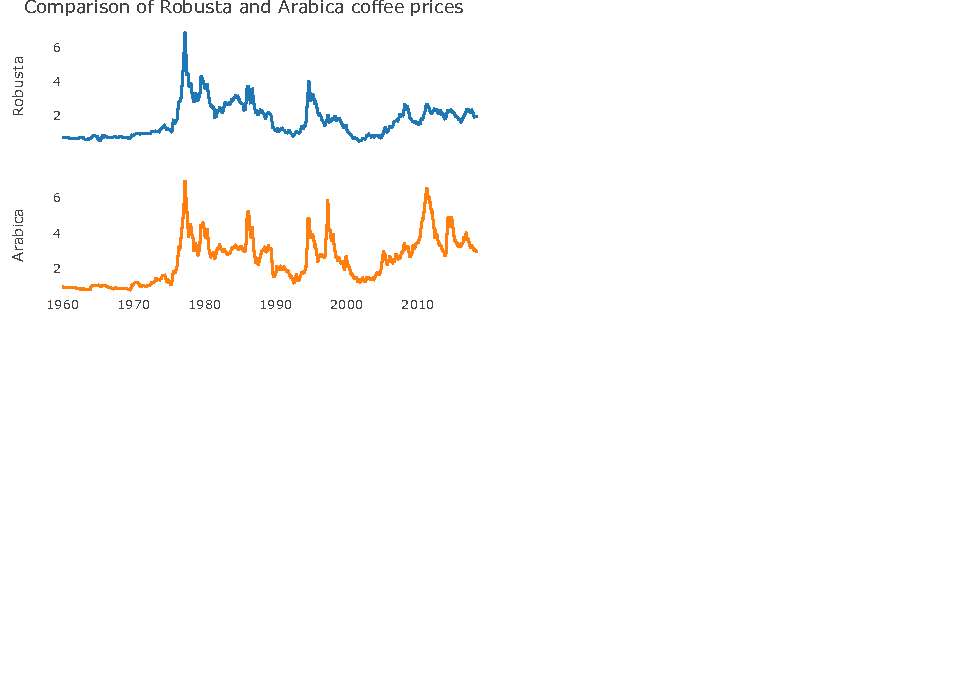
\includegraphics{_main_files/figure-latex/unnamed-chunk-65-1.pdf}

\textbf{Note} that the \textbf{color}, \textbf{Ytitle}, and \textbf{Xtitle} arguments are not applicable when plotting multiple time series object.

\section{Practical Examples: Exercises}\label{practical-examples-exercises-2}

\textbf{Exercise 13: Stock market data}

Obtain the daily closing prices for the last ten calendar years of S\&P 500 Index, Dow Jones, NASDAQ100 and Russell 2000 indices from Yahoo Finance using the appropriate R package such as tidyquant or quantmod. Prepare the data and clean it by removing any missing values. Plot a time series plot of the prices of these indices in one graph and use the plot to identify any economic trends among the indices.

\textbf{Exercise 14: Temperature}

Obtain the temperature data from an open source such as Weather data (\url{https://www.wunderground.com/weather/in/ahmedabad/VAAH}) for Ahmedabad which is located in Western India on the banks of River Sabarmati. Obtain the average monthly temperature data from Sardar Vallabhbhai Patel International Airport Station weather station for the years 2014-2021. Decompose the time series data by splitting these components (data or the level, trend, seasonality, and noise or random components) separately into
individual components. Present the decomposition of the multiplicative model of the components of the time series of the average
temperature of Ahmedabad in a suitable plot. What observation did you make about the seasonality of this data?

\chapter{STATISTICAL GRAPHS IN R}\label{statistical-graphs-in-r}

\section{Introduction}\label{introduction-4}

The two main objectives of this chapter are:

\begin{itemize}
\tightlist
\item
  Learn to use R's base graphics for creating statistical plots.
\item
  Understand the application of statistical plots in real-world data analysis.
\end{itemize}

\section{Essential Statistical Plots:}\label{essential-statistical-plots}

Statistical plots are essential for exploring and understanding the distribution of data. In this chapter, we will cover how to create the following essential statistical plots in R and understand the insights they provide.

\subsection{How to create box plots, violin plots, and QQ plots.}\label{how-to-create-box-plots-violin-plots-and-qq-plots.}

\textbf{i) Box Plots:}

\begin{Shaded}
\begin{Highlighting}[]
\CommentTok{\# Creating a box plot}
\FunctionTok{boxplot}\NormalTok{(Sepal.Length }\SpecialCharTok{\textasciitilde{}}\NormalTok{ Species, }\AttributeTok{data =}\NormalTok{ iris, }
        \AttributeTok{main =} \StringTok{"Box Plot of Sepal Length by Species"}\NormalTok{,}
        \AttributeTok{xlab =} \StringTok{"Species"}\NormalTok{, }\AttributeTok{ylab =} \StringTok{"Sepal Length"}\NormalTok{)}
\end{Highlighting}
\end{Shaded}

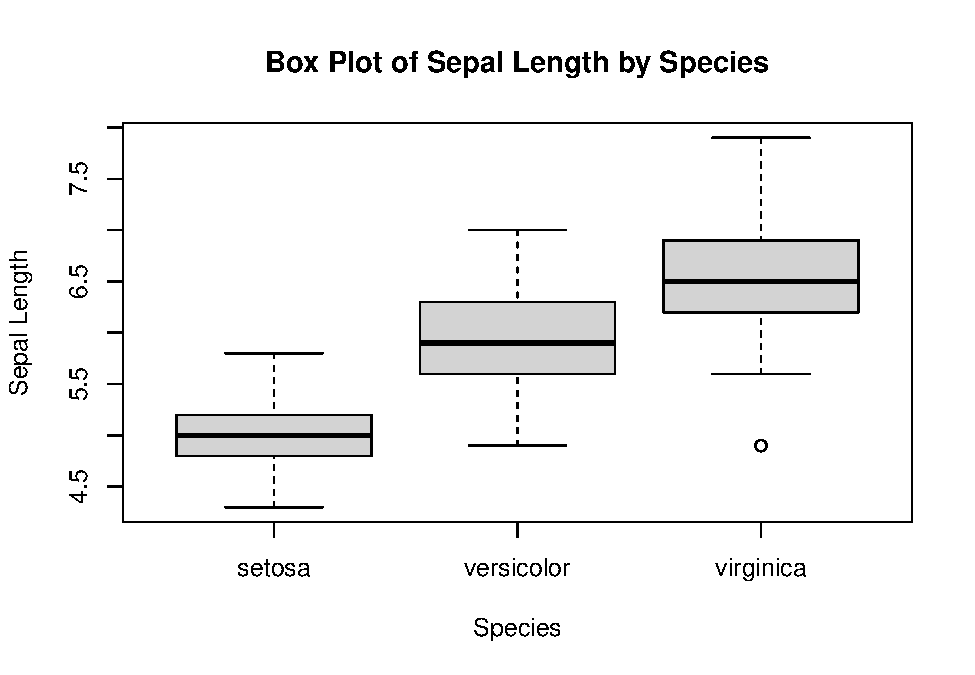
\includegraphics{_main_files/figure-latex/unnamed-chunk-67-1.pdf}

\textbf{ii) Violin Plots:}

\begin{Shaded}
\begin{Highlighting}[]
\CommentTok{\# Creating a violin plot}
\FunctionTok{library}\NormalTok{(ggplot2)}
\FunctionTok{ggplot}\NormalTok{(iris, }\FunctionTok{aes}\NormalTok{(}\AttributeTok{x =}\NormalTok{ Species, }\AttributeTok{y =}\NormalTok{ Sepal.Length)) }\SpecialCharTok{+}
  \FunctionTok{geom\_violin}\NormalTok{(}\AttributeTok{fill =} \StringTok{"lightblue"}\NormalTok{) }\SpecialCharTok{+}
  \FunctionTok{labs}\NormalTok{(}\AttributeTok{title =} \StringTok{"Violin Plot of Sepal Length by Species"}\NormalTok{,}
       \AttributeTok{x =} \StringTok{"Species"}\NormalTok{, }\AttributeTok{y =} \StringTok{"Sepal Length"}\NormalTok{)}
\end{Highlighting}
\end{Shaded}

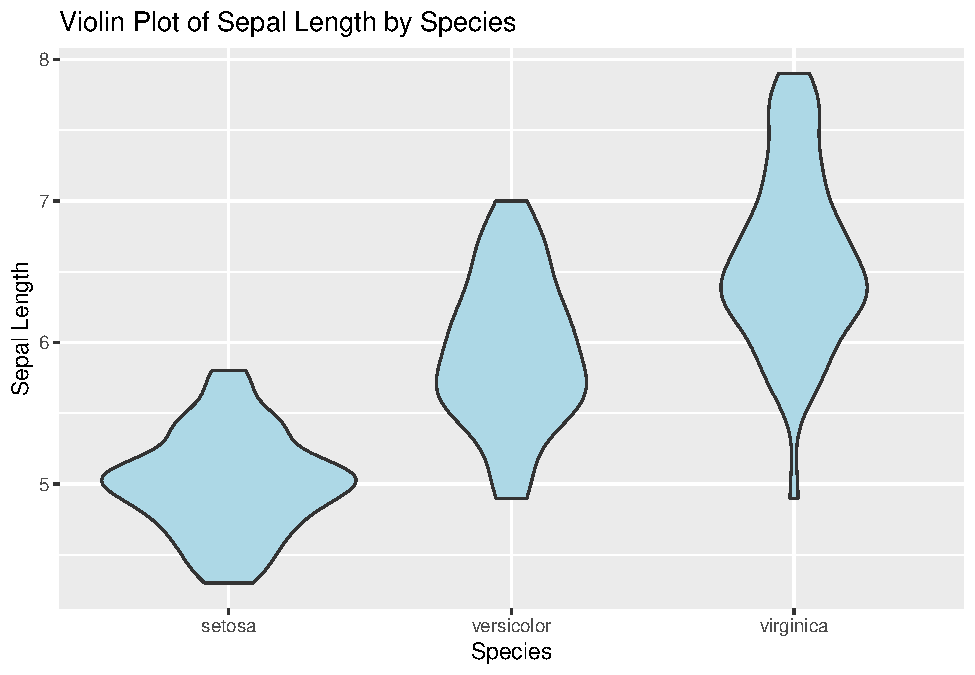
\includegraphics{_main_files/figure-latex/unnamed-chunk-68-1.pdf}

\textbf{iii) QQ Plots:}

\begin{Shaded}
\begin{Highlighting}[]
\CommentTok{\# Creating a QQ plot}
\FunctionTok{qqnorm}\NormalTok{(iris}\SpecialCharTok{$}\NormalTok{Sepal.Length)}
\FunctionTok{qqline}\NormalTok{(iris}\SpecialCharTok{$}\NormalTok{Sepal.Length)}
\end{Highlighting}
\end{Shaded}

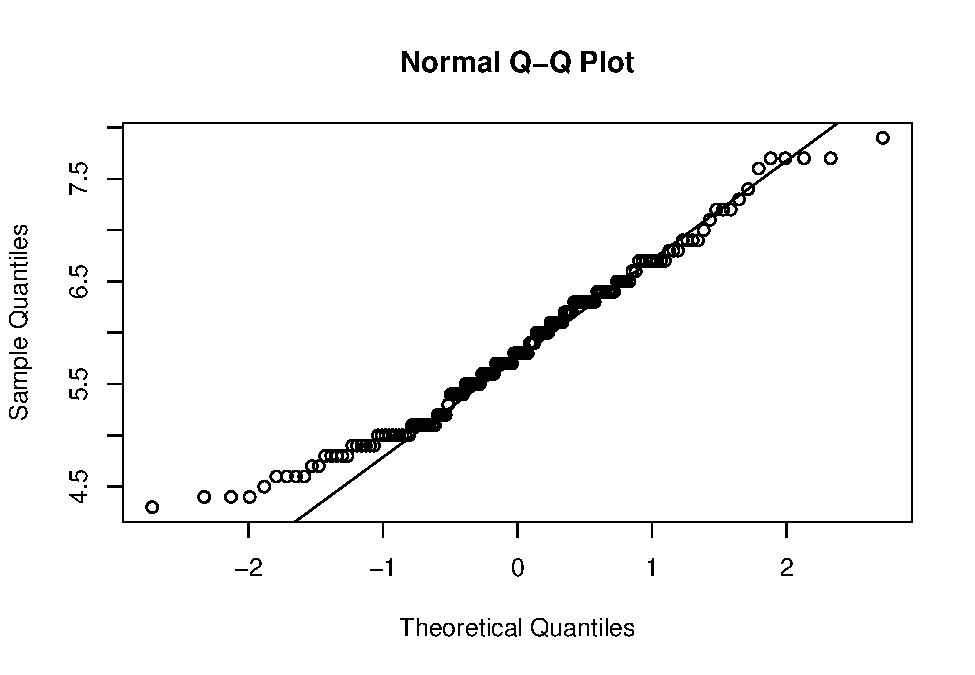
\includegraphics{_main_files/figure-latex/unnamed-chunk-69-1.pdf}

\subsection{Understanding the data insights these plots provide.}\label{understanding-the-data-insights-these-plots-provide.}

\textbf{i) Box Plots:} Box plots provide a graphical summary of the distribution of a dataset. They display the median, quartiles, and potential outliers.

\textbf{ii) Violin Plots:} Violin plots are similar to box plots but provide a more detailed summary of the distribution. They combine a box plot with a kernel density plot.

\textbf{iii) QQ Plots (Quantile-Quantile Plots):} QQ plots are used to assess if a dataset follows a particular distribution. They compare the quantiles of the dataset against the quantiles of a theoretical distribution.

These statistical plots are invaluable tools for exploring and understanding the distribution of data.

\section{Analyzing Distributions with Histograms and Density Plots:}\label{analyzing-distributions-with-histograms-and-density-plots}

Histograms provide a visual representation of the distribution of numerical data. They group data into bins and display the frequency of observations in each bin.Density plots estimate the probability density function of the underlying data distribution. They provide a smooth representation of the distribution.

\subsection{Techniques for creating and customizing histograms and density plots and best practices for displaying distribution characteristics.}\label{techniques-for-creating-and-customizing-histograms-and-density-plots-and-best-practices-for-displaying-distribution-characteristics.}

\textbf{Creating and Customizing Histograms:}

\begin{Shaded}
\begin{Highlighting}[]
\CommentTok{\# Creating a histogram}
\FunctionTok{hist}\NormalTok{(iris}\SpecialCharTok{$}\NormalTok{Sepal.Length, }
     \AttributeTok{main =} \StringTok{"Histogram of Sepal Length"}\NormalTok{,}
     \AttributeTok{xlab =} \StringTok{"Sepal Length"}\NormalTok{,}
     \AttributeTok{ylab =} \StringTok{"Frequency"}\NormalTok{,}
     \AttributeTok{col =} \StringTok{"lightblue"}\NormalTok{)}

\CommentTok{\# Adding a density plot}
\FunctionTok{lines}\NormalTok{(}\FunctionTok{density}\NormalTok{(iris}\SpecialCharTok{$}\NormalTok{Sepal.Length), }\AttributeTok{col =} \StringTok{"red"}\NormalTok{)}
\end{Highlighting}
\end{Shaded}

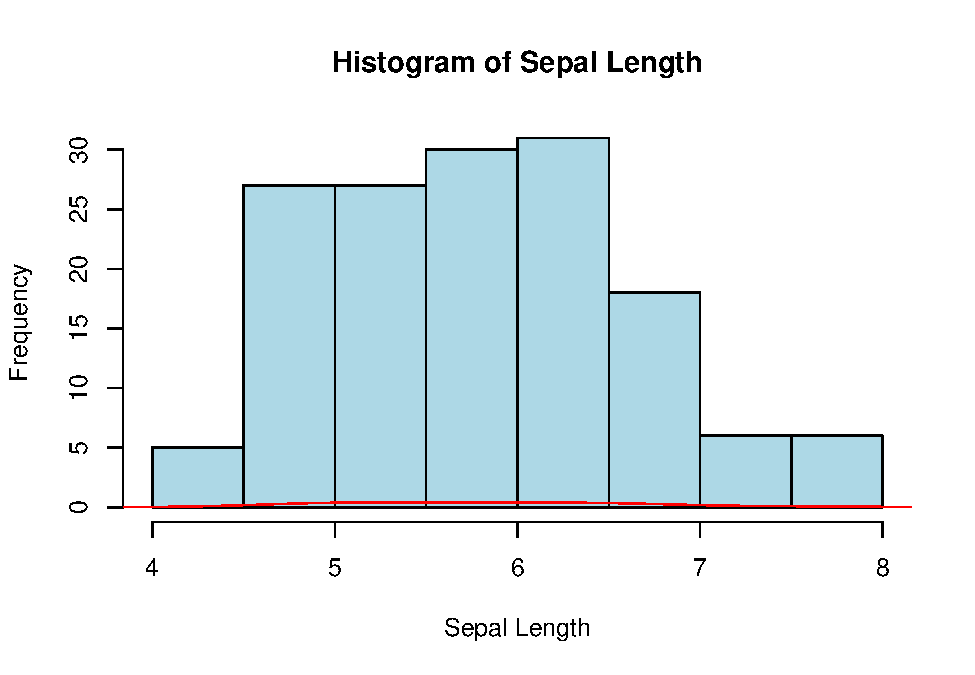
\includegraphics{_main_files/figure-latex/unnamed-chunk-70-1.pdf}

\textbf{Creating and Customizing Density Plots:}

\begin{Shaded}
\begin{Highlighting}[]
\CommentTok{\# Creating a density plot}
\FunctionTok{plot}\NormalTok{(}\FunctionTok{density}\NormalTok{(iris}\SpecialCharTok{$}\NormalTok{Sepal.Length), }
     \AttributeTok{main =} \StringTok{"Density Plot of Sepal Length"}\NormalTok{,}
     \AttributeTok{xlab =} \StringTok{"Sepal Length"}\NormalTok{,}
     \AttributeTok{col =} \StringTok{"blue"}\NormalTok{)}

\CommentTok{\# Adding a histogram}
\FunctionTok{hist}\NormalTok{(iris}\SpecialCharTok{$}\NormalTok{Sepal.Length, }
     \AttributeTok{col =} \FunctionTok{rgb}\NormalTok{(}\DecValTok{0}\NormalTok{,}\DecValTok{0}\NormalTok{,}\DecValTok{1}\NormalTok{,}\FloatTok{0.2}\NormalTok{), }
     \AttributeTok{add =} \ConstantTok{TRUE}\NormalTok{, }
     \AttributeTok{breaks =} \DecValTok{20}\NormalTok{)}
\end{Highlighting}
\end{Shaded}

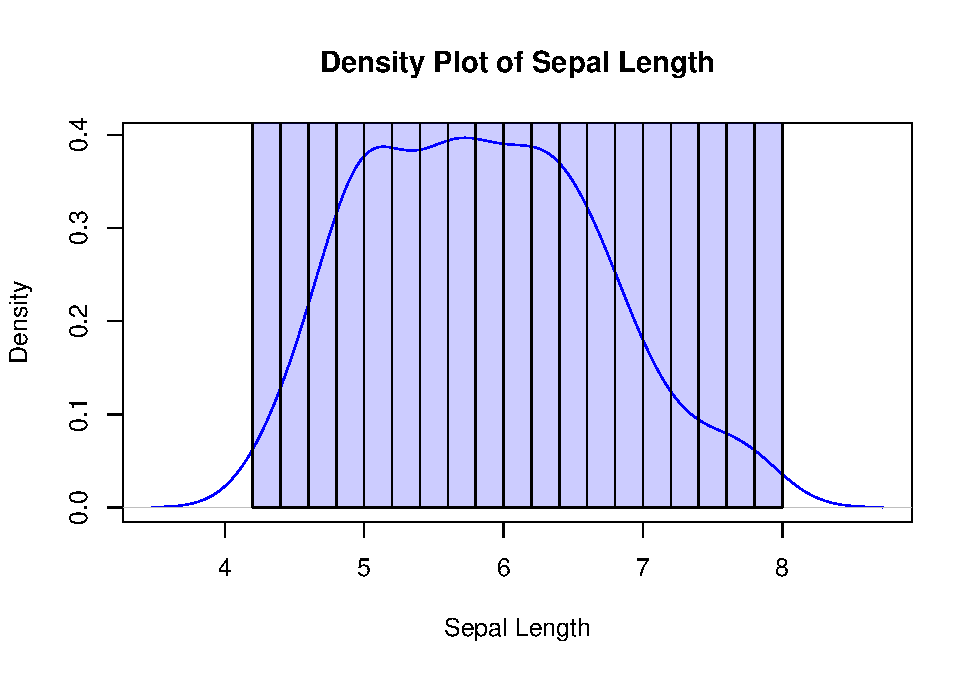
\includegraphics{_main_files/figure-latex/unnamed-chunk-71-1.pdf}

\section{Scatter Plots and Correlation Analysis:}\label{scatter-plots-and-correlation-analysis}

Scatter plots are useful for visualizing the relationship between two continuous variables.

\subsection{Using scatter plots to visualize relationships between variables.}\label{using-scatter-plots-to-visualize-relationships-between-variables.}

Scatter plots visually represent the relationship between two continuous variables. They help to identify patterns, trends, and correlations between variables.

\begin{Shaded}
\begin{Highlighting}[]
\CommentTok{\# Creating a scatter plot}
\FunctionTok{plot}\NormalTok{(iris}\SpecialCharTok{$}\NormalTok{Sepal.Length, iris}\SpecialCharTok{$}\NormalTok{Petal.Length,}
     \AttributeTok{main =} \StringTok{"Scatter Plot of Sepal Length vs Petal Length"}\NormalTok{,}
     \AttributeTok{xlab =} \StringTok{"Sepal Length"}\NormalTok{, }\AttributeTok{ylab =} \StringTok{"Petal Length"}\NormalTok{,}
     \AttributeTok{col =} \StringTok{"blue"}\NormalTok{)}
\end{Highlighting}
\end{Shaded}

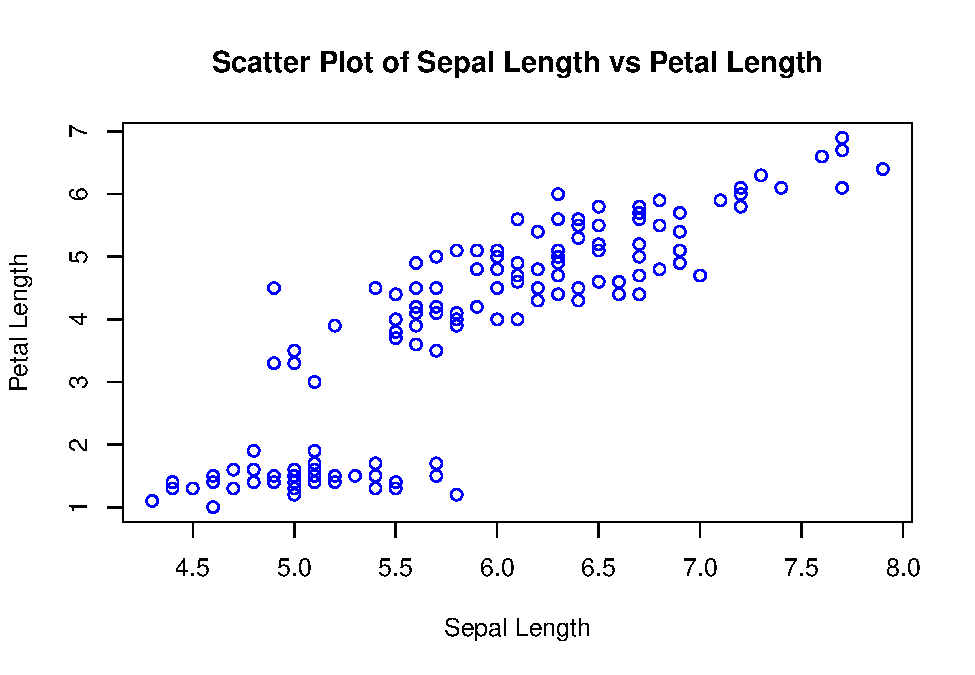
\includegraphics{_main_files/figure-latex/unnamed-chunk-72-1.pdf}

\subsection{Introduction to adding regression lines and confidence intervals.}\label{introduction-to-adding-regression-lines-and-confidence-intervals.}

\begin{itemize}
\item
  Regression lines provide a summary of the relationship between variables.
\item
  Confidence intervals help assess the uncertainty of the estimated regression line.
\end{itemize}

\begin{Shaded}
\begin{Highlighting}[]
\CommentTok{\# Creating a scatter plot}
\FunctionTok{plot}\NormalTok{(iris}\SpecialCharTok{$}\NormalTok{Sepal.Length, iris}\SpecialCharTok{$}\NormalTok{Petal.Length,}
     \AttributeTok{main =} \StringTok{"Scatter Plot and Regression Line of Sepal Length vs Petal Length"}\NormalTok{,}
     \AttributeTok{xlab =} \StringTok{"Sepal Length"}\NormalTok{, }\AttributeTok{ylab =} \StringTok{"Petal Length"}\NormalTok{,}
     \AttributeTok{col =} \StringTok{"blue"}\NormalTok{)}

\CommentTok{\# Fit linear regression model}
\NormalTok{model }\OtherTok{\textless{}{-}} \FunctionTok{lm}\NormalTok{(Petal.Length }\SpecialCharTok{\textasciitilde{}}\NormalTok{ Sepal.Length, }\AttributeTok{data =}\NormalTok{ iris)}

\CommentTok{\# Adding regression line}
\FunctionTok{abline}\NormalTok{(model, }\AttributeTok{col =} \StringTok{"red"}\NormalTok{)}

\CommentTok{\# Adding regression equation}
\NormalTok{eq }\OtherTok{\textless{}{-}} \FunctionTok{paste}\NormalTok{(}\StringTok{"y ="}\NormalTok{, }\FunctionTok{round}\NormalTok{(}\FunctionTok{coef}\NormalTok{(model)[}\DecValTok{1}\NormalTok{], }\DecValTok{2}\NormalTok{), }\StringTok{"+"}\NormalTok{, }\FunctionTok{round}\NormalTok{(}\FunctionTok{coef}\NormalTok{(model)[}\DecValTok{2}\NormalTok{], }\DecValTok{2}\NormalTok{), }\StringTok{"x"}\NormalTok{)}
\FunctionTok{text}\NormalTok{(}\FloatTok{6.5}\NormalTok{, }\FloatTok{2.5}\NormalTok{, eq, }\AttributeTok{pos =} \DecValTok{4}\NormalTok{)}

\CommentTok{\# Adding confidence intervals}
\NormalTok{conf\_interval }\OtherTok{\textless{}{-}} \FunctionTok{predict}\NormalTok{(model, }\AttributeTok{interval =} \StringTok{"confidence"}\NormalTok{)}
\FunctionTok{lines}\NormalTok{(iris}\SpecialCharTok{$}\NormalTok{Sepal.Length, conf\_interval[, }\StringTok{"lwr"}\NormalTok{], }\AttributeTok{col =} \StringTok{"green"}\NormalTok{, }\AttributeTok{lty =} \DecValTok{2}\NormalTok{)}
\FunctionTok{lines}\NormalTok{(iris}\SpecialCharTok{$}\NormalTok{Sepal.Length, conf\_interval[, }\StringTok{"upr"}\NormalTok{], }\AttributeTok{col =} \StringTok{"green"}\NormalTok{, }\AttributeTok{lty =} \DecValTok{2}\NormalTok{)}
\CommentTok{\# Add legend}
\FunctionTok{legend}\NormalTok{(}\StringTok{"topleft"}\NormalTok{, }\AttributeTok{legend =} \FunctionTok{c}\NormalTok{(}\StringTok{"Data Points"}\NormalTok{, }\StringTok{"Regression Line"}\NormalTok{, }\StringTok{"Confidence Intervals"}\NormalTok{),}
       \AttributeTok{col =} \FunctionTok{c}\NormalTok{(}\StringTok{"blue"}\NormalTok{, }\StringTok{"red"}\NormalTok{, }\StringTok{"green"}\NormalTok{), }\AttributeTok{lty =} \FunctionTok{c}\NormalTok{(}\ConstantTok{NA}\NormalTok{, }\DecValTok{1}\NormalTok{, }\DecValTok{2}\NormalTok{), }\AttributeTok{lwd =} \FunctionTok{c}\NormalTok{(}\ConstantTok{NA}\NormalTok{, }\DecValTok{1}\NormalTok{, }\DecValTok{1}\NormalTok{),}
       \AttributeTok{pch =} \FunctionTok{c}\NormalTok{(}\DecValTok{1}\NormalTok{, }\ConstantTok{NA}\NormalTok{, }\ConstantTok{NA}\NormalTok{), }\AttributeTok{bty =} \StringTok{"o"} \CommentTok{\# Enclose the legend in a box}
\NormalTok{       )}
\end{Highlighting}
\end{Shaded}

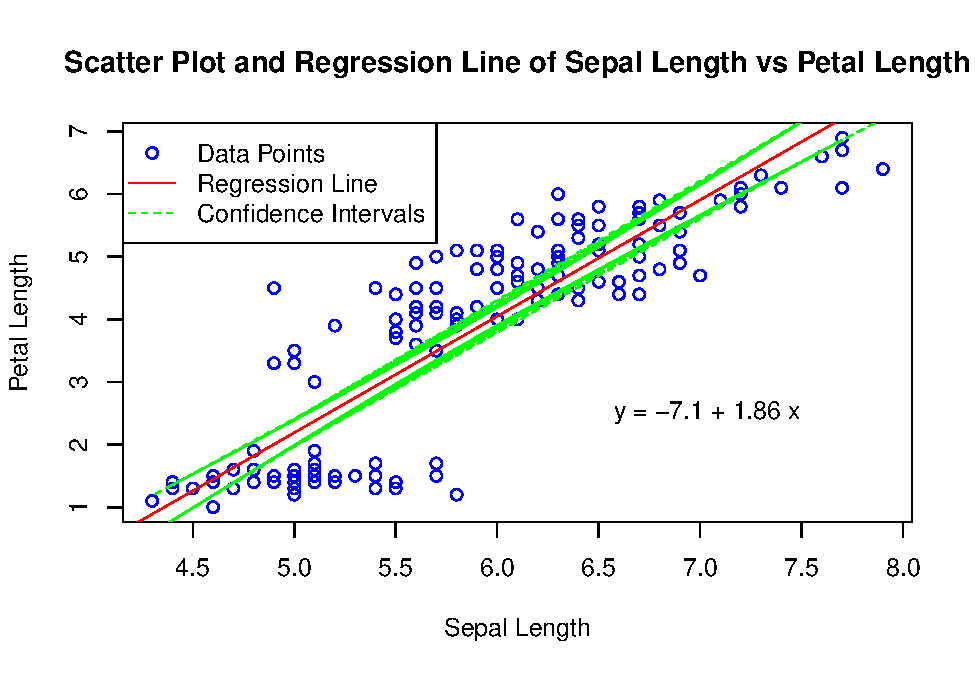
\includegraphics{_main_files/figure-latex/unnamed-chunk-73-1.pdf}

\section{Practical Examples: Exercises}\label{practical-examples-exercises-3}

\chapter{INTRODUCTION TO ggplot2}\label{introduction-to-ggplot2}

\section{Getting Started with ggplot2}\label{getting-started-with-ggplot2}

\subsection{Installation of ggplot2 and setting up the environment.}\label{installation-of-ggplot2-and-setting-up-the-environment.}

If you have not installed the \textbf{ggplot2} package in your computer, then installing the package for the first time is achieved by writing the code \textbf{install.packages(``ggplot2'')}. Once, the package has successfully been installed, you can set up the environment to use it in your analysis by writing the code \textbf{library(``ggplot2'')}. Alternatively, \textbf{ggpot2} package can be loaded by loading the \textbf{tidyverse} package which comes while attached with several packages where ggplot2 is among them.

\subsection{Basic syntax and components of ggplot2: aesthetics, geoms, and layers}\label{basic-syntax-and-components-of-ggplot2-aesthetics-geoms-and-layers}

\begin{itemize}
\item
  \textbf{Aesthetics:} Mapping data variables to visual properties.
\item
  \textbf{Geoms:} Geometric objects that represent data points, lines, shapes, etc.
\item
  \textbf{Layers:} Building plots by adding layers of graphics.
\end{itemize}

\section{Creating Basic Plots with ggplot2}\label{creating-basic-plots-with-ggplot2}

We are using the gapminder dataset (\url{https://www.gapminder.org/data}) that has
been put into an R package by Bryan (2017) so we can load it with
library(gapminder). The dataset includes 1704 observations (rows) of 6 variables (columns: country,
continent, year, lifeExp, pop, gdpPercap). country, continent, and year could
be thought of as grouping variables, whereas lifeExp (life expectancy), pop
(population), and gdpPercap (Gross Domestic Product per capita) are values.
The years in this dataset span 1952 to 2007 with 5-year intervals (so a total of
12 different years). It includes 142 countries from 5 continents (Asia, Europe,
Africa, Americas, Oceania).
You can check that all of the numbers quoted above are correct with these
lines:

\begin{Shaded}
\begin{Highlighting}[]
\FunctionTok{library}\NormalTok{(tidyverse)}
\FunctionTok{library}\NormalTok{(gapminder)}
\NormalTok{gapminder}\SpecialCharTok{$}\NormalTok{year }\SpecialCharTok{\%\textgreater{}\%} \FunctionTok{unique}\NormalTok{()}
\end{Highlighting}
\end{Shaded}

\begin{verbatim}
##  [1] 1952 1957 1962 1967 1972 1977 1982 1987 1992 1997 2002 2007
\end{verbatim}

\begin{Shaded}
\begin{Highlighting}[]
\NormalTok{gapminder}\SpecialCharTok{$}\NormalTok{country }\SpecialCharTok{\%\textgreater{}\%} \FunctionTok{n\_distinct}\NormalTok{()}
\end{Highlighting}
\end{Shaded}

\begin{verbatim}
## [1] 142
\end{verbatim}

\begin{Shaded}
\begin{Highlighting}[]
\NormalTok{gapminder}\SpecialCharTok{$}\NormalTok{continent }\SpecialCharTok{\%\textgreater{}\%} \FunctionTok{unique}\NormalTok{()}
\end{Highlighting}
\end{Shaded}

\begin{verbatim}
## [1] Asia     Europe   Africa   Americas Oceania 
## Levels: Africa Americas Asia Europe Oceania
\end{verbatim}

\subsection{Step-by-step instructions to create scatter plots, histograms, and bar charts using ggplot2}\label{step-by-step-instructions-to-create-scatter-plots-histograms-and-bar-charts-using-ggplot2}

\subsubsection{Scatter plots/bubble plots}\label{scatter-plotsbubble-plots}

Let's create a new shorter tibble called gapdata2007 that only includes data for the year 2007. Let's ask ggplot() to draw a point for each observation by adding geom\_point()

\begin{Shaded}
\begin{Highlighting}[]
\CommentTok{\# Filter only the year 2007 data}
\NormalTok{gapdata2007 }\OtherTok{\textless{}{-}}\NormalTok{ gapminder }\SpecialCharTok{\%\textgreater{}\%}
\FunctionTok{filter}\NormalTok{(year }\SpecialCharTok{==} \DecValTok{2007}\NormalTok{)}

\CommentTok{\#Plot a simple scatter plot }
\NormalTok{gapdata2007 }\SpecialCharTok{\%\textgreater{}\%}
\FunctionTok{ggplot}\NormalTok{(}\FunctionTok{aes}\NormalTok{(}\AttributeTok{x =}\NormalTok{ gdpPercap, }\AttributeTok{y =}\NormalTok{ lifeExp)) }\SpecialCharTok{+}
\FunctionTok{geom\_point}\NormalTok{()}
\end{Highlighting}
\end{Shaded}

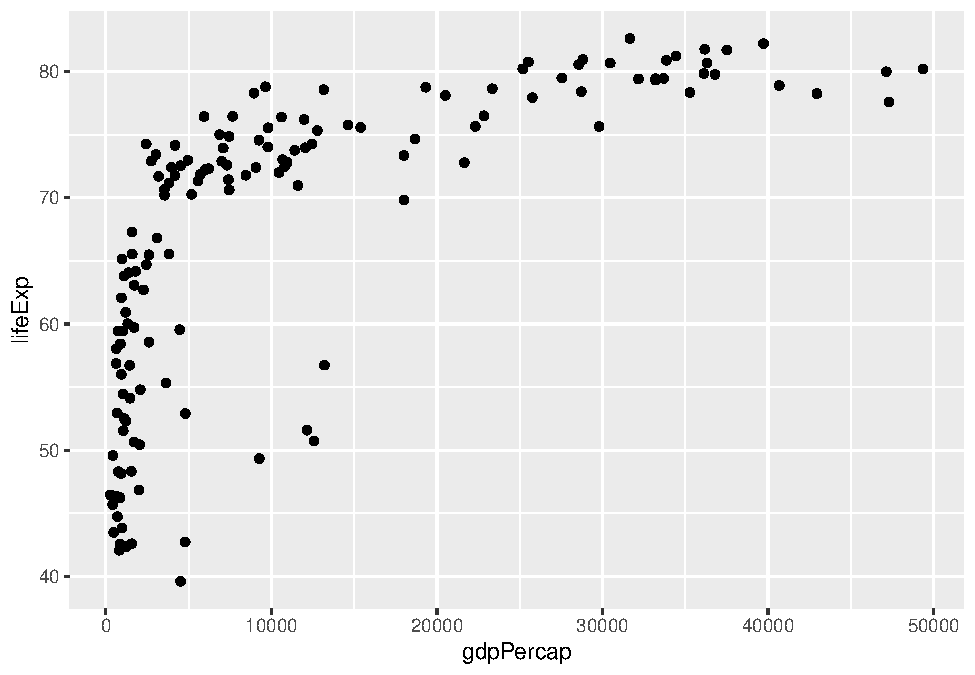
\includegraphics{_main_files/figure-latex/unnamed-chunk-76-1.pdf}

\subsubsection{Histograms}\label{histograms}

A histogram displays the distribution of values within a continuous variable.
In the example below, we are taking the life expectancy (aes(x = lifeExp))
and telling the histogram to count the observations up in ``bins'' of 10 years
(geom\_histogram(binwidth = 10)

\begin{Shaded}
\begin{Highlighting}[]
\NormalTok{gapdata2007 }\SpecialCharTok{\%\textgreater{}\%}
\FunctionTok{ggplot}\NormalTok{(}\FunctionTok{aes}\NormalTok{(}\AttributeTok{x =}\NormalTok{ lifeExp)) }\SpecialCharTok{+}
\FunctionTok{geom\_histogram}\NormalTok{(}\AttributeTok{binwidth =} \DecValTok{10}\NormalTok{)}
\end{Highlighting}
\end{Shaded}

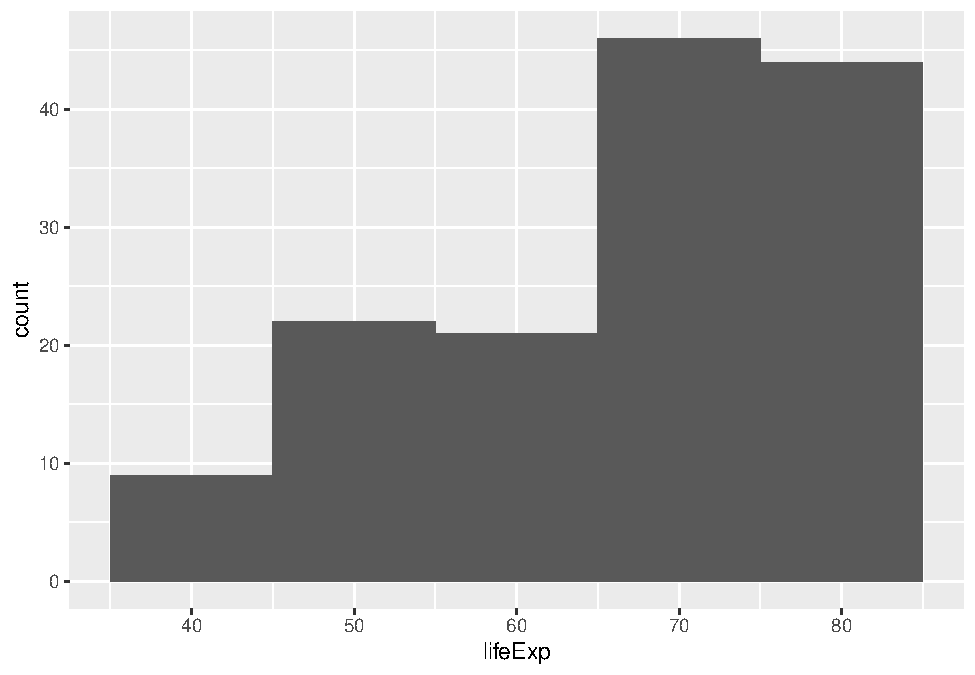
\includegraphics{_main_files/figure-latex/unnamed-chunk-77-1.pdf}

We can see that most countries in the world have a life expectancy of \textasciitilde70-80
years (in 2007), and that the distribution of life expectancy globally is not normally distributed. Setting the binwidth is optional, using just geom\_histogram() works well too - by default, it will divide the data into 30 bins.

\subsubsection{Bar plots}\label{bar-plots}

There are two geoms for making bar plots - \textbf{geom\_col()} and \textbf{geom\_bar()} and the examples below will illustrate when to use which one. In short: if your data is already summarised or includes values for y (height of the bars), use \textbf{geom\_col()}. If, however, you want ggplot() to count up the number of rows in your dataset, use \textbf{geom\_bar()}. For example, with patient-level data (each row is a patient) you'll probably want to use geom\_bar(), with data that is already somewhat aggregated, you'll use geom\_col(). There is no harm in trying one, and if it doesn't work, trying the other.

Let's plot the life expectancies in 2007 in these three countries:

\begin{Shaded}
\begin{Highlighting}[]
\NormalTok{gapdata2007 }\SpecialCharTok{\%\textgreater{}\%}
\FunctionTok{filter}\NormalTok{(country }\SpecialCharTok{\%in\%} \FunctionTok{c}\NormalTok{(}\StringTok{"United Kingdom"}\NormalTok{, }\StringTok{"France"}\NormalTok{, }\StringTok{"Germany"}\NormalTok{)) }\SpecialCharTok{\%\textgreater{}\%}
\FunctionTok{ggplot}\NormalTok{(}\FunctionTok{aes}\NormalTok{(}\AttributeTok{x =}\NormalTok{ country, }\AttributeTok{y =}\NormalTok{ lifeExp)) }\SpecialCharTok{+}
\FunctionTok{geom\_col}\NormalTok{()}
\end{Highlighting}
\end{Shaded}

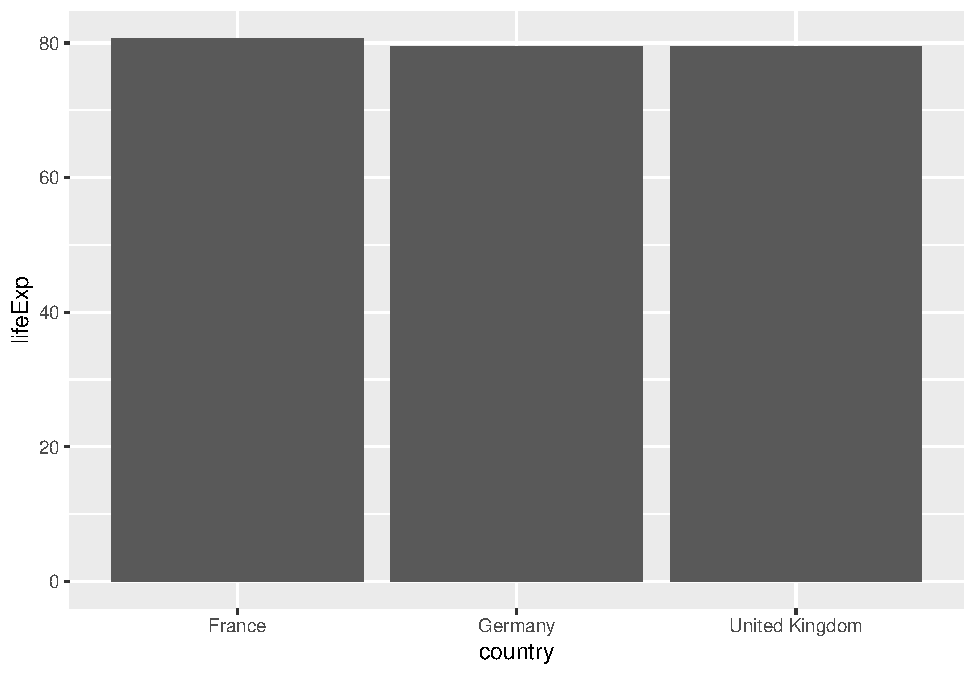
\includegraphics{_main_files/figure-latex/unnamed-chunk-78-1.pdf}

\subsubsection{Box plots}\label{box-plots}

Box plots are our go to method for quickly visualizing summary statistics of a continuous outcome variable (such as life expectancy in the gapminder dataset. Box plots include:

\begin{itemize}
\tightlist
\item
  the median (middle line in the box)
\item
  inter-quartile range (IQR, top and bottom parts of the boxes - this is where
  50\% of your data is)
\item
  whiskers (the black lines extending to the lowest and highest values that are
  still within 1.5*IQR)
\item
  outliers (any observations out with the whiskers)
\end{itemize}

Let's pot the boxplots of life expectancies within each continent in year 2007

\begin{Shaded}
\begin{Highlighting}[]
\NormalTok{gapdata2007 }\SpecialCharTok{\%\textgreater{}\%}
\FunctionTok{ggplot}\NormalTok{(}\FunctionTok{aes}\NormalTok{(}\AttributeTok{x =}\NormalTok{ continent, }\AttributeTok{y =}\NormalTok{ lifeExp)) }\SpecialCharTok{+}
\FunctionTok{geom\_boxplot}\NormalTok{()}
\end{Highlighting}
\end{Shaded}

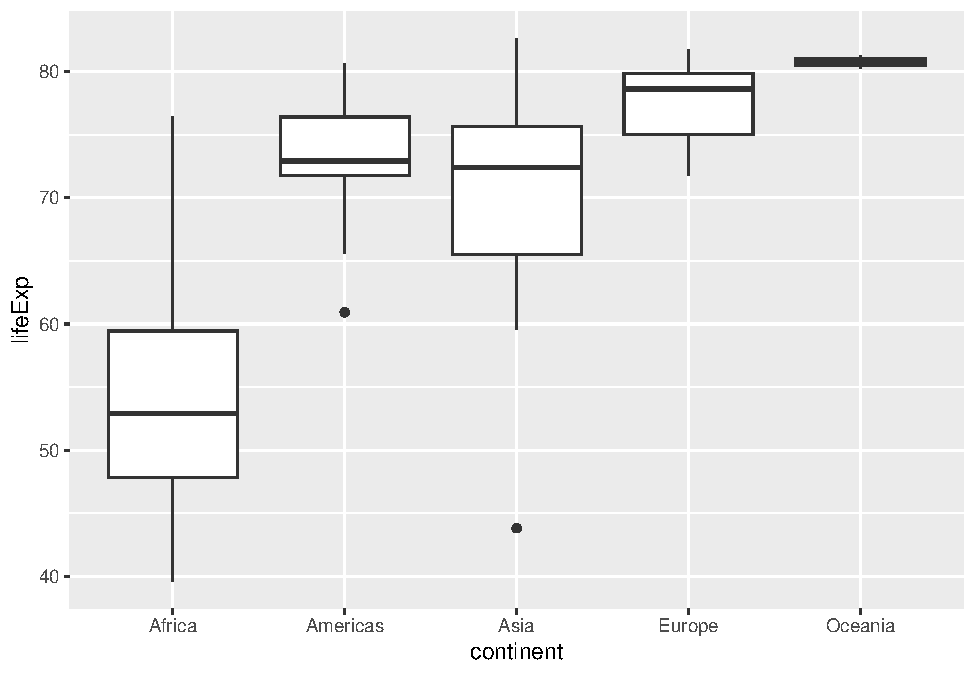
\includegraphics{_main_files/figure-latex/unnamed-chunk-79-1.pdf}

\subsubsection{Line plots/time series plots}\label{line-plotstime-series-plots}

Let's plot the life expectancy in the United Kingdom over time.

\begin{Shaded}
\begin{Highlighting}[]
\NormalTok{gapdata }\OtherTok{\textless{}{-}}\NormalTok{ gapminder}
\NormalTok{gapdata }\SpecialCharTok{\%\textgreater{}\%}
\FunctionTok{filter}\NormalTok{(country }\SpecialCharTok{==} \StringTok{"United Kingdom"}\NormalTok{) }\SpecialCharTok{\%\textgreater{}\%}
\FunctionTok{ggplot}\NormalTok{(}\FunctionTok{aes}\NormalTok{(}\AttributeTok{x =}\NormalTok{ year, }\AttributeTok{y =}\NormalTok{ lifeExp)) }\SpecialCharTok{+}
\FunctionTok{geom\_line}\NormalTok{()}
\end{Highlighting}
\end{Shaded}

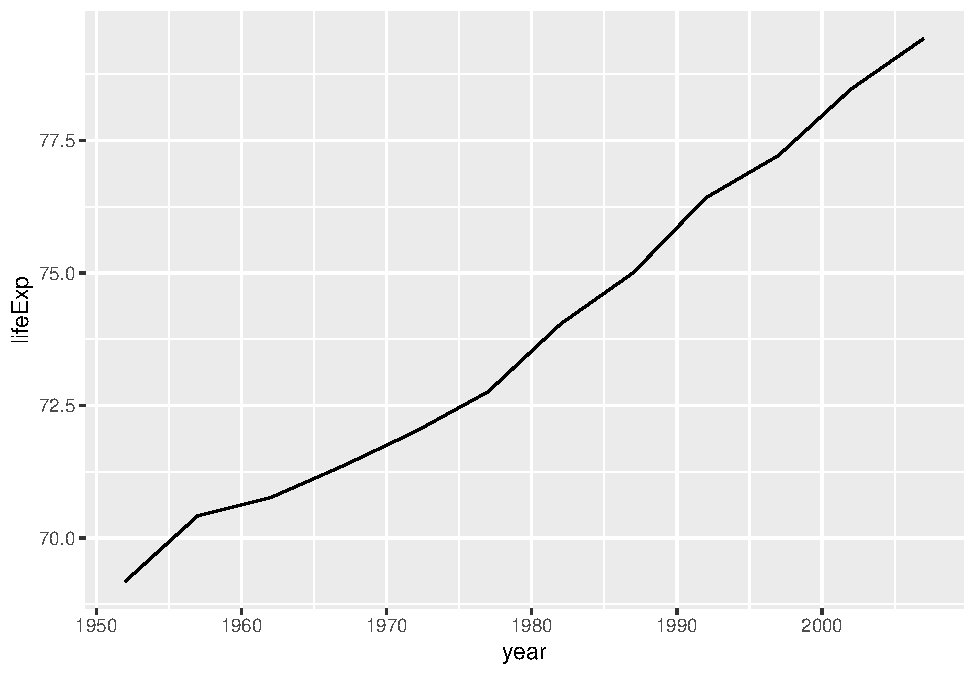
\includegraphics{_main_files/figure-latex/unnamed-chunk-80-1.pdf}

\subsection{Introduction to adding layers, modifying aesthetics, and utilizing facets for multi-panel plots}\label{introduction-to-adding-layers-modifying-aesthetics-and-utilizing-facets-for-multi-panel-plots}

\textbf{a) Adding layers}

Going back to the scatter plot (lifeExp vs gdpPercap), let's use continent to give the points some colour. We can do this by adding colour = continent inside the aes():Let's also add a regression line to the scatter plot

\begin{Shaded}
\begin{Highlighting}[]
\NormalTok{gapdata2007 }\SpecialCharTok{\%\textgreater{}\%}
\FunctionTok{ggplot}\NormalTok{(}\FunctionTok{aes}\NormalTok{(}\AttributeTok{x =}\NormalTok{ gdpPercap, }\AttributeTok{y =}\NormalTok{ lifeExp, }\AttributeTok{colour =}\NormalTok{ continent)) }\SpecialCharTok{+}
\FunctionTok{geom\_point}\NormalTok{()}\SpecialCharTok{+}
\FunctionTok{geom\_smooth}\NormalTok{(}\AttributeTok{method =} \StringTok{"lm"}\NormalTok{, }\AttributeTok{se =} \ConstantTok{FALSE}\NormalTok{)}
\end{Highlighting}
\end{Shaded}

\begin{verbatim}
## `geom_smooth()` using formula = 'y ~ x'
\end{verbatim}

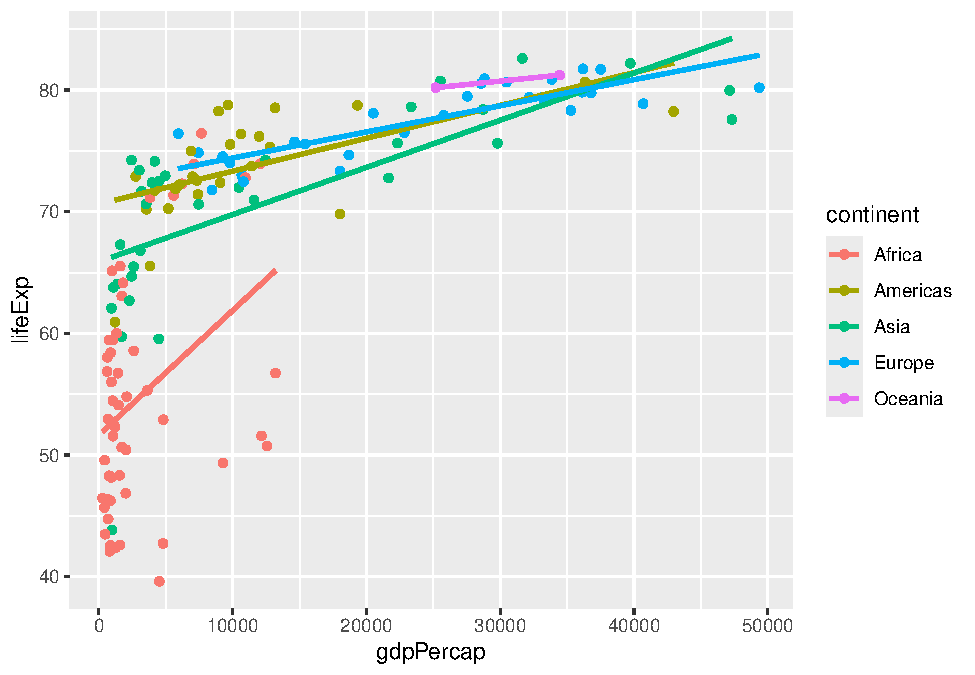
\includegraphics{_main_files/figure-latex/unnamed-chunk-81-1.pdf}

\textbf{b) Modifying aesthetics}

This can be achieved by specifying further variables inside \textbf{aes()} or specifying aesthetics outside \textbf{aes()}. The main aesthetics (things we can see) are: \textbf{x, y, colour, fill, shape, size,} and any of these could appear inside or outside the \textbf{aes()} function.

Variables (so columns of your dataset) have to be defined inside \textbf{aes()}. Whereas to apply a modification on everything, we can set an aesthetic to a constant value outside of aes().

\begin{Shaded}
\begin{Highlighting}[]
\NormalTok{gapdata2007 }\SpecialCharTok{\%\textgreater{}\%}
\FunctionTok{ggplot}\NormalTok{(}\FunctionTok{aes}\NormalTok{(}\AttributeTok{x =}\NormalTok{ gdpPercap, }\AttributeTok{y =}\NormalTok{ lifeExp, }\AttributeTok{colour =}\NormalTok{ continent)) }\SpecialCharTok{+}
\FunctionTok{geom\_point}\NormalTok{(}\AttributeTok{shape =} \DecValTok{1}\NormalTok{)}
\end{Highlighting}
\end{Shaded}

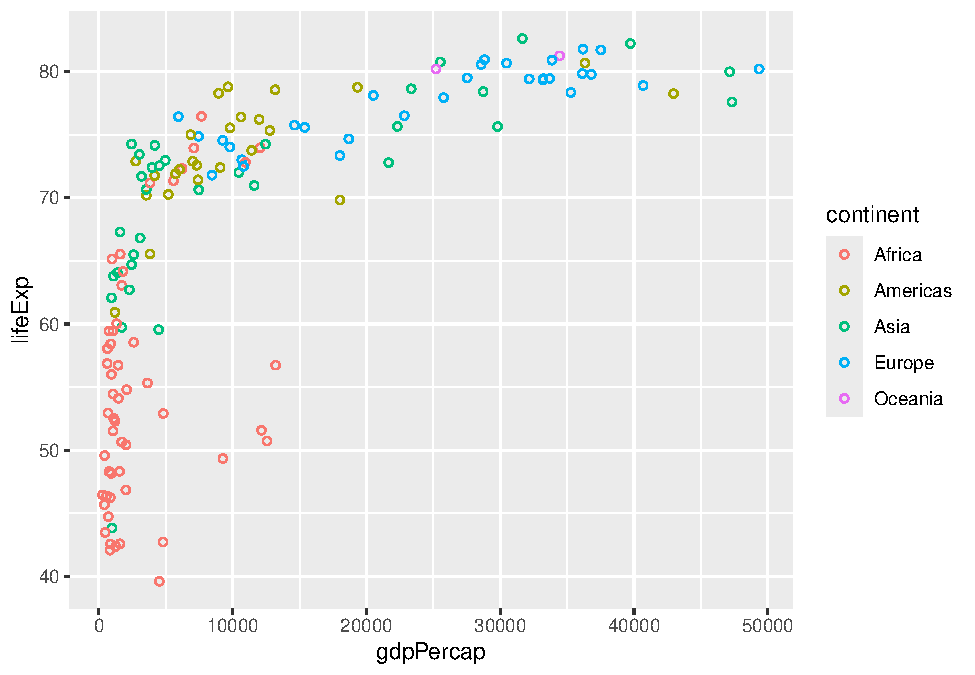
\includegraphics{_main_files/figure-latex/unnamed-chunk-82-1.pdf}

\textbf{c) Utilizing facets for multi-panel plots}
Faceting is a way to efficiently create the same plot for subgroups within the dataset. For example, we can separate each continent into its own facet by adding facet\_wrap(\textasciitilde continent) to our plot:

\begin{Shaded}
\begin{Highlighting}[]
\NormalTok{gapdata2007 }\SpecialCharTok{\%\textgreater{}\%}
\FunctionTok{ggplot}\NormalTok{(}\FunctionTok{aes}\NormalTok{(}\AttributeTok{x =}\NormalTok{ gdpPercap, }\AttributeTok{y =}\NormalTok{ lifeExp, }\AttributeTok{colour =}\NormalTok{ continent)) }\SpecialCharTok{+}
\FunctionTok{geom\_point}\NormalTok{(}\AttributeTok{shape =} \DecValTok{1}\NormalTok{) }\SpecialCharTok{+}
\FunctionTok{facet\_wrap}\NormalTok{(}\SpecialCharTok{\textasciitilde{}}\NormalTok{continent)}
\end{Highlighting}
\end{Shaded}

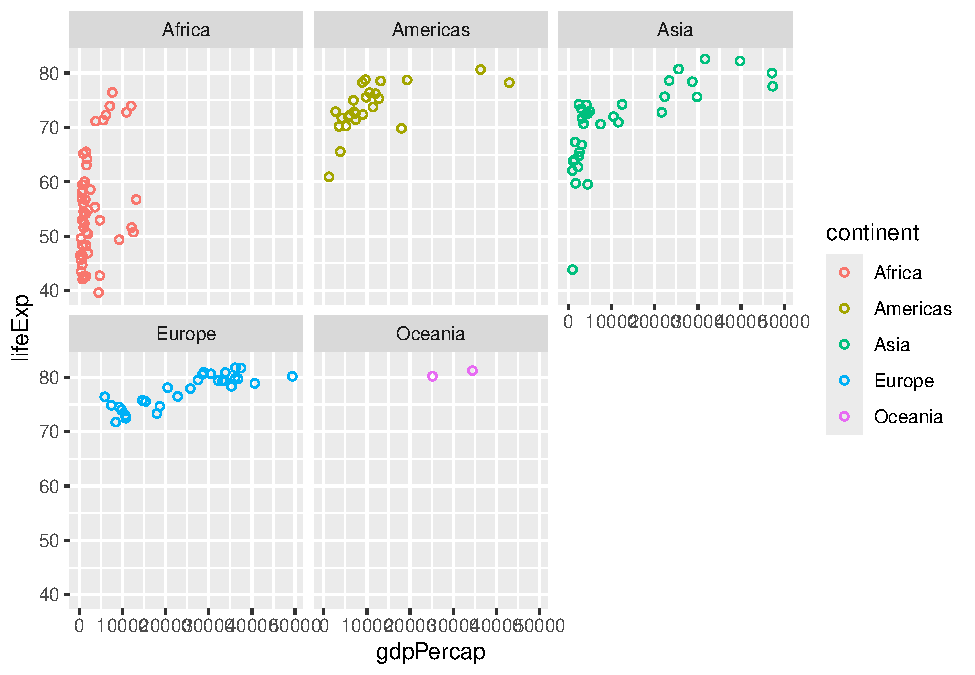
\includegraphics{_main_files/figure-latex/unnamed-chunk-83-1.pdf}

\section{Customizing Plots in ggplot2}\label{customizing-plots-in-ggplot2}

\subsection{Advanced customization techniques including themes, scales, and coordinate systems.}\label{advanced-customization-techniques-including-themes-scales-and-coordinate-systems.}

\textbf{a) Themes}

Changing themes involves changing the default background from grey to a white background. Some of the built-in ggplot themes are \textbf{theme\_bw()},
\textbf{theme\_dark()}, \textbf{theme\_minimal()} and \textbf{theme\_classic()}. We are adding \textbf{theme\_bw()} (``background white'') to give the plot a different look. We have also divided the gdpPercap by 1000 (making the units ``thousands of dollars per capita''). Note that you can apply calculations
directly on ggplot variables (so how we've done x = gdpPercap/1000 here). This is how ggplot() works - you can build a plot by adding or modifying things one by one.

\begin{Shaded}
\begin{Highlighting}[]
\NormalTok{gapdata2007 }\SpecialCharTok{\%\textgreater{}\%}
\FunctionTok{ggplot}\NormalTok{(}\FunctionTok{aes}\NormalTok{(}\AttributeTok{x =}\NormalTok{ gdpPercap}\SpecialCharTok{/}\DecValTok{1000}\NormalTok{, }\AttributeTok{y =}\NormalTok{ lifeExp, }\AttributeTok{colour =}\NormalTok{ continent)) }\SpecialCharTok{+}
\FunctionTok{geom\_point}\NormalTok{(}\AttributeTok{shape =} \DecValTok{1}\NormalTok{) }\SpecialCharTok{+}
\FunctionTok{facet\_wrap}\NormalTok{(}\SpecialCharTok{\textasciitilde{}}\NormalTok{continent) }\SpecialCharTok{+}
\FunctionTok{theme\_bw}\NormalTok{()}
\end{Highlighting}
\end{Shaded}

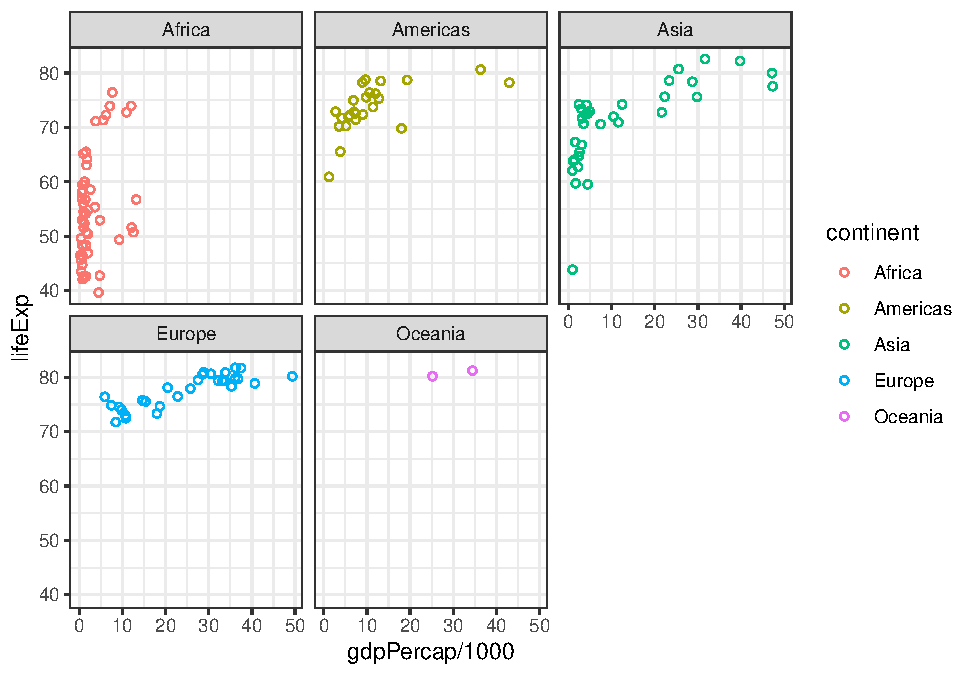
\includegraphics{_main_files/figure-latex/unnamed-chunk-84-1.pdf}

\textbf{b) Scales}

\begin{Shaded}
\begin{Highlighting}[]
\NormalTok{gapminder }\SpecialCharTok{\%\textgreater{}\%}
\FunctionTok{ggplot}\NormalTok{(}\FunctionTok{aes}\NormalTok{(}\AttributeTok{x =}\NormalTok{ year, }\AttributeTok{y =}\NormalTok{ lifeExp, }\AttributeTok{group =}\NormalTok{ country, }\AttributeTok{colour =}\NormalTok{ continent)) }\SpecialCharTok{+}
\FunctionTok{geom\_line}\NormalTok{() }\SpecialCharTok{+}
\FunctionTok{facet\_wrap}\NormalTok{(}\SpecialCharTok{\textasciitilde{}}\NormalTok{continent) }\SpecialCharTok{+}
\FunctionTok{theme\_bw}\NormalTok{() }\SpecialCharTok{+}
\FunctionTok{scale\_colour\_brewer}\NormalTok{(}\AttributeTok{palette =} \StringTok{"Paired"}\NormalTok{)}
\end{Highlighting}
\end{Shaded}

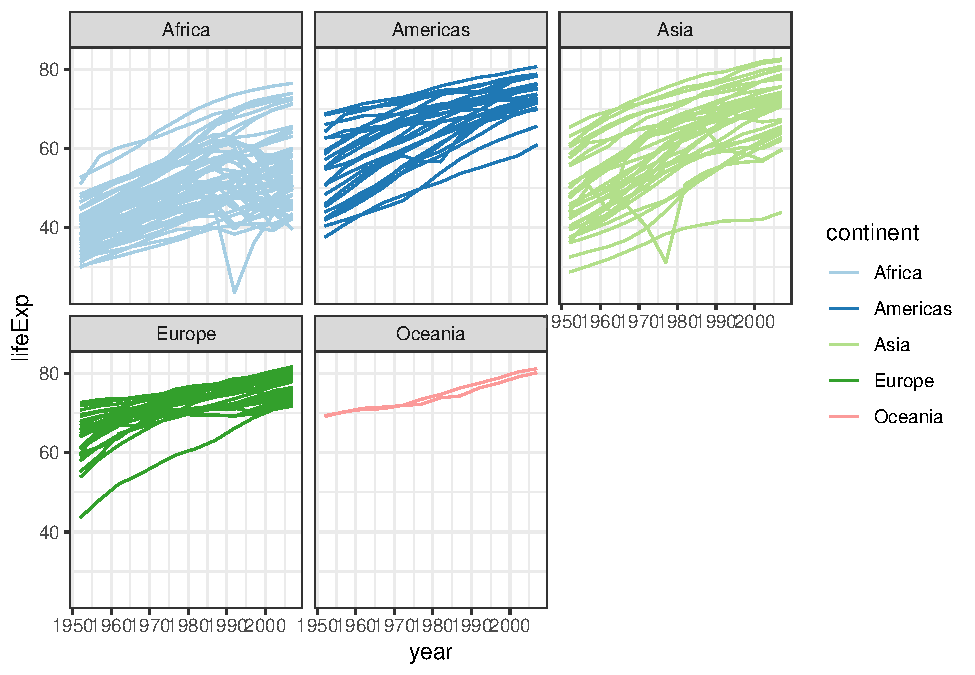
\includegraphics{_main_files/figure-latex/unnamed-chunk-85-1.pdf}

\textbf{c) Coordinate systems}

\begin{Shaded}
\begin{Highlighting}[]
\CommentTok{\# Flipped coordinate system}
\NormalTok{gapdata2007 }\SpecialCharTok{\%\textgreater{}\%}
\FunctionTok{ggplot}\NormalTok{(}\FunctionTok{aes}\NormalTok{(}\AttributeTok{x =}\NormalTok{ gdpPercap, }\AttributeTok{y =}\NormalTok{ lifeExp, }\AttributeTok{colour =}\NormalTok{ continent)) }\SpecialCharTok{+}
\FunctionTok{geom\_point}\NormalTok{(}\AttributeTok{shape =} \DecValTok{1}\NormalTok{)}\SpecialCharTok{+}
  \FunctionTok{coord\_flip}\NormalTok{() }\SpecialCharTok{+}
  \FunctionTok{labs}\NormalTok{(}\AttributeTok{title =} \StringTok{"Scatter Plot with Flipped Coordinate System"}\NormalTok{,}
       \AttributeTok{x =} \StringTok{"GDP Per Capita"}\NormalTok{, }\AttributeTok{y =} \StringTok{"Life Expectancy"}\NormalTok{) }\SpecialCharTok{+}
  \FunctionTok{theme\_bw}\NormalTok{()}
\end{Highlighting}
\end{Shaded}

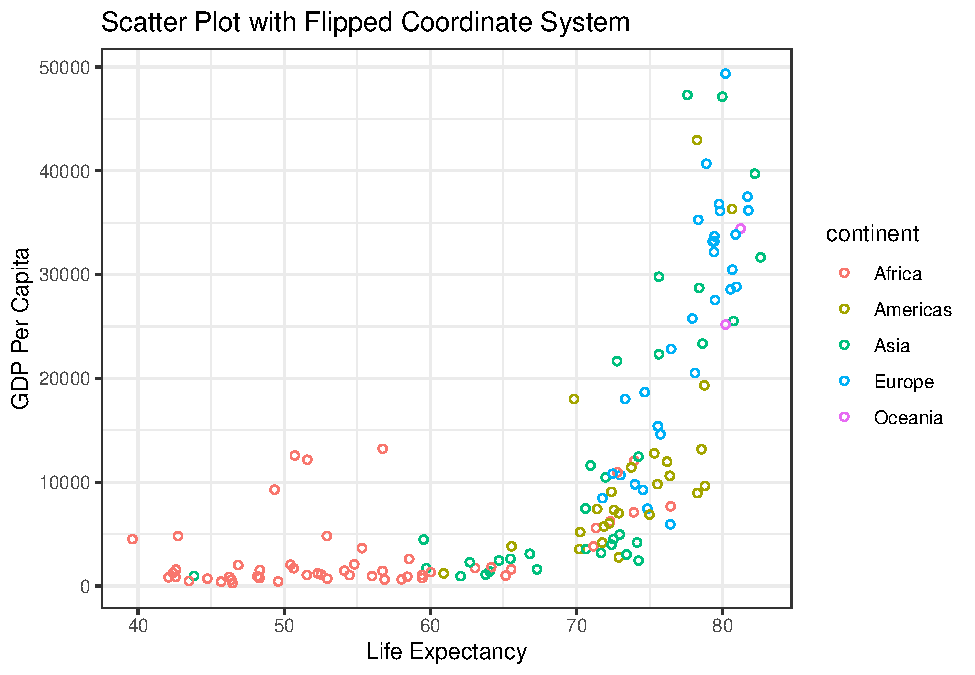
\includegraphics{_main_files/figure-latex/unnamed-chunk-86-1.pdf}

\subsection{Techniques for fine-tuning ggplot2 outputs to create publication-quality graphics}\label{techniques-for-fine-tuning-ggplot2-outputs-to-create-publication-quality-graphics}

\begin{Shaded}
\begin{Highlighting}[]
\CommentTok{\# Publication{-}quality scatter plot}
\FunctionTok{ggplot}\NormalTok{(}\AttributeTok{data =}\NormalTok{ iris, }\FunctionTok{aes}\NormalTok{(}\AttributeTok{x =}\NormalTok{ Sepal.Length, }\AttributeTok{y =}\NormalTok{ Sepal.Width, }\AttributeTok{color =}\NormalTok{ Species)) }\SpecialCharTok{+} 
  \FunctionTok{geom\_point}\NormalTok{(}\AttributeTok{alpha =} \FloatTok{0.7}\NormalTok{, }\AttributeTok{size =} \DecValTok{3}\NormalTok{) }\SpecialCharTok{+}
  \FunctionTok{labs}\NormalTok{(}\AttributeTok{title =} \StringTok{"Publication{-}Quality Scatter Plot"}\NormalTok{,}
       \AttributeTok{x =} \StringTok{"Sepal Length"}\NormalTok{, }\AttributeTok{y =} \StringTok{"Sepal Width"}\NormalTok{) }\SpecialCharTok{+}
  \FunctionTok{theme\_bw}\NormalTok{() }\SpecialCharTok{+}
  \FunctionTok{theme}\NormalTok{(}
    \AttributeTok{plot.title =} \FunctionTok{element\_text}\NormalTok{(}\AttributeTok{size =} \DecValTok{14}\NormalTok{, }\AttributeTok{face =} \StringTok{"bold"}\NormalTok{, }\AttributeTok{hjust =} \FloatTok{0.5}\NormalTok{),}
    \AttributeTok{axis.title =} \FunctionTok{element\_text}\NormalTok{(}\AttributeTok{size =} \DecValTok{12}\NormalTok{),}
    \AttributeTok{axis.text =} \FunctionTok{element\_text}\NormalTok{(}\AttributeTok{size =} \DecValTok{10}\NormalTok{),}
    \AttributeTok{legend.title =} \FunctionTok{element\_text}\NormalTok{(}\AttributeTok{size =} \DecValTok{12}\NormalTok{),}
    \AttributeTok{legend.text =} \FunctionTok{element\_text}\NormalTok{(}\AttributeTok{size =} \DecValTok{10}\NormalTok{)}
\NormalTok{  ) }\SpecialCharTok{+}
  \FunctionTok{scale\_color\_manual}\NormalTok{(}\AttributeTok{values =} \FunctionTok{c}\NormalTok{(}\StringTok{"setosa"} \OtherTok{=} \StringTok{"blue"}\NormalTok{, }\StringTok{"versicolor"} \OtherTok{=} \StringTok{"green"}\NormalTok{, }\StringTok{"virginica"} \OtherTok{=} \StringTok{"red"}\NormalTok{))}
\end{Highlighting}
\end{Shaded}

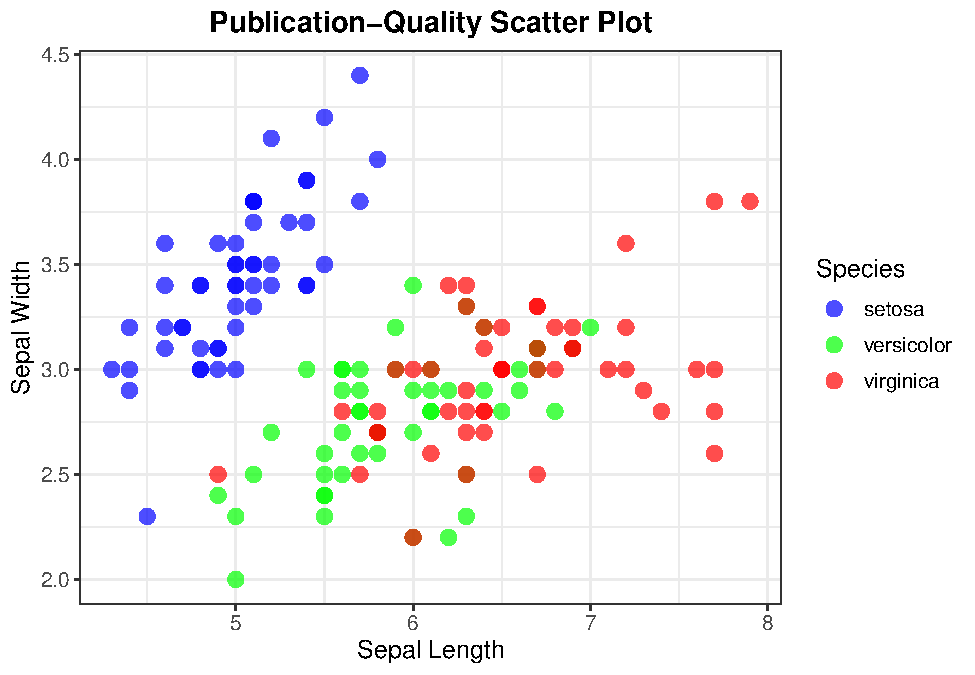
\includegraphics{_main_files/figure-latex/unnamed-chunk-87-1.pdf}

\section{Practical Examples: Exercise}\label{practical-examples-exercise-1}

\chapter{ADVANCED DATA VISUALIZATION WITH ggplot2 AND OTHER PACKAGES}\label{advanced-data-visualization-with-ggplot2-and-other-packages}

\section{Interactive Graphs with plotly}\label{interactive-graphs-with-plotly}

\subsection{Converting ggplot2 charts into interactive plotly graphs}\label{converting-ggplot2-charts-into-interactive-plotly-graphs}

Before converting the ggplot2 chart to interactive plotly graph, you assign the plot to a vector, say, p.~Then load the \textbf{plotly} package and convert the ggplot chart to interactive plotly graph using the \textbf{ggpotly()} function, for example, \textbf{ggplotly(p)}.

\begin{Shaded}
\begin{Highlighting}[]
\FunctionTok{library}\NormalTok{(plotly)}
\NormalTok{p}\OtherTok{\textless{}{-}}\FunctionTok{ggplot}\NormalTok{(}\AttributeTok{data =}\NormalTok{ iris, }\FunctionTok{aes}\NormalTok{(}\AttributeTok{x =}\NormalTok{ Sepal.Length, }\AttributeTok{y =}\NormalTok{ Sepal.Width, }\AttributeTok{color =}\NormalTok{ Species)) }\SpecialCharTok{+} 
  \FunctionTok{geom\_point}\NormalTok{(}\AttributeTok{alpha =} \FloatTok{0.7}\NormalTok{, }\AttributeTok{size =} \DecValTok{3}\NormalTok{) }\SpecialCharTok{+}
  \FunctionTok{labs}\NormalTok{(}\AttributeTok{title =} \StringTok{"Publication{-}Quality Scatter Plot"}\NormalTok{,}
       \AttributeTok{x =} \StringTok{"Sepal Length"}\NormalTok{, }\AttributeTok{y =} \StringTok{"Sepal Width"}\NormalTok{) }\SpecialCharTok{+}
  \FunctionTok{theme\_bw}\NormalTok{() }\SpecialCharTok{+}
  \FunctionTok{theme}\NormalTok{(}
    \AttributeTok{plot.title =} \FunctionTok{element\_text}\NormalTok{(}\AttributeTok{size =} \DecValTok{14}\NormalTok{, }\AttributeTok{face =} \StringTok{"bold"}\NormalTok{, }\AttributeTok{hjust =} \FloatTok{0.5}\NormalTok{),}
    \AttributeTok{axis.title =} \FunctionTok{element\_text}\NormalTok{(}\AttributeTok{size =} \DecValTok{12}\NormalTok{),}
    \AttributeTok{axis.text =} \FunctionTok{element\_text}\NormalTok{(}\AttributeTok{size =} \DecValTok{10}\NormalTok{),}
    \AttributeTok{legend.title =} \FunctionTok{element\_text}\NormalTok{(}\AttributeTok{size =} \DecValTok{12}\NormalTok{),}
    \AttributeTok{legend.text =} \FunctionTok{element\_text}\NormalTok{(}\AttributeTok{size =} \DecValTok{10}\NormalTok{)}
\NormalTok{  ) }\SpecialCharTok{+}
  \FunctionTok{scale\_color\_manual}\NormalTok{(}\AttributeTok{values =} \FunctionTok{c}\NormalTok{(}\StringTok{"setosa"} \OtherTok{=} \StringTok{"blue"}\NormalTok{, }\StringTok{"versicolor"} \OtherTok{=} \StringTok{"green"}\NormalTok{, }\StringTok{"virginica"} \OtherTok{=} \StringTok{"red"}\NormalTok{))}

\CommentTok{\# Convert ggplot2 to plotly}
\CommentTok{\#ggplotly(p)}
\end{Highlighting}
\end{Shaded}

\subsection{Customizing interactions, adding tooltips, and embedding plotly graphs in web applications.}\label{customizing-interactions-adding-tooltips-and-embedding-plotly-graphs-in-web-applications.}

\textbf{Customizing Interactions and Adding Tooltips}

\begin{Shaded}
\begin{Highlighting}[]
\CommentTok{\# Convert ggplot2 scatter plot to plotly with custom tooltip}
\NormalTok{p }\OtherTok{\textless{}{-}} \FunctionTok{ggplot}\NormalTok{(}\AttributeTok{data =}\NormalTok{ iris, }\FunctionTok{aes}\NormalTok{(}\AttributeTok{x =}\NormalTok{ Sepal.Length, }\AttributeTok{y =}\NormalTok{ Sepal.Width, }\AttributeTok{color =}\NormalTok{ Species, }
                             \AttributeTok{text =} \FunctionTok{paste}\NormalTok{(}\StringTok{"Species: "}\NormalTok{, Species))) }\SpecialCharTok{+} 
  \FunctionTok{geom\_point}\NormalTok{() }\SpecialCharTok{+}
  \FunctionTok{labs}\NormalTok{(}\AttributeTok{title =} \StringTok{"Interactive Scatter Plot of Sepal Length vs Sepal Width"}\NormalTok{,}
       \AttributeTok{x =} \StringTok{"Sepal Length"}\NormalTok{, }\AttributeTok{y =} \StringTok{"Sepal Width"}\NormalTok{) }\SpecialCharTok{+}
  \FunctionTok{theme\_bw}\NormalTok{()}

\CommentTok{\# Convert ggplot2 to plotly with custom tooltip}
\CommentTok{\#ggplotly(p, tooltip = "text")}
\end{Highlighting}
\end{Shaded}

\textbf{Embedding plotly Graphs in Web Applications (Shiny)}

\begin{Shaded}
\begin{Highlighting}[]
\CommentTok{\# Install and load Shiny package}
\CommentTok{\#install.packages("shiny")}
\FunctionTok{library}\NormalTok{(shiny)}
\end{Highlighting}
\end{Shaded}

\begin{verbatim}
## Warning: package 'shiny' was built under R version 4.3.3
\end{verbatim}

\begin{Shaded}
\begin{Highlighting}[]
\CommentTok{\# Define UI}
\NormalTok{ui }\OtherTok{\textless{}{-}} \FunctionTok{fluidPage}\NormalTok{(}
  \FunctionTok{titlePanel}\NormalTok{(}\StringTok{"Interactive Scatter Plot"}\NormalTok{),}
  \FunctionTok{plotlyOutput}\NormalTok{(}\StringTok{"scatter\_plot"}\NormalTok{)}
\NormalTok{)}

\CommentTok{\# Define server logic}
\NormalTok{server }\OtherTok{\textless{}{-}} \ControlFlowTok{function}\NormalTok{(input, output) \{}
\NormalTok{  output}\SpecialCharTok{$}\NormalTok{scatter\_plot }\OtherTok{\textless{}{-}} \FunctionTok{renderPlotly}\NormalTok{(\{}
    \FunctionTok{ggplot}\NormalTok{(}\AttributeTok{data =}\NormalTok{ iris, }\FunctionTok{aes}\NormalTok{(}\AttributeTok{x =}\NormalTok{ Sepal.Length, }\AttributeTok{y =}\NormalTok{ Sepal.Width, }\AttributeTok{color =}\NormalTok{ Species, }
                            \AttributeTok{text =} \FunctionTok{paste}\NormalTok{(}\StringTok{"Species: "}\NormalTok{, Species))) }\SpecialCharTok{+} 
      \FunctionTok{geom\_point}\NormalTok{() }\SpecialCharTok{+}
      \FunctionTok{labs}\NormalTok{(}\AttributeTok{title =} \StringTok{"Interactive Scatter Plot of Sepal Length vs Sepal Width"}\NormalTok{,}
           \AttributeTok{x =} \StringTok{"Sepal Length"}\NormalTok{, }\AttributeTok{y =} \StringTok{"Sepal Width"}\NormalTok{) }\SpecialCharTok{+}
      \FunctionTok{theme\_minimal}\NormalTok{() }\SpecialCharTok{\%\textgreater{}\%}
      \FunctionTok{ggplotly}\NormalTok{(}\AttributeTok{tooltip =} \StringTok{"text"}\NormalTok{)}
\NormalTok{  \})}
\NormalTok{\}}

\CommentTok{\# Run the application}
\FunctionTok{shinyApp}\NormalTok{(}\AttributeTok{ui =}\NormalTok{ ui, }\AttributeTok{server =}\NormalTok{ server)}
\end{Highlighting}
\end{Shaded}

\begin{verbatim}
## 
## Listening on http://127.0.0.1:3755
\end{verbatim}

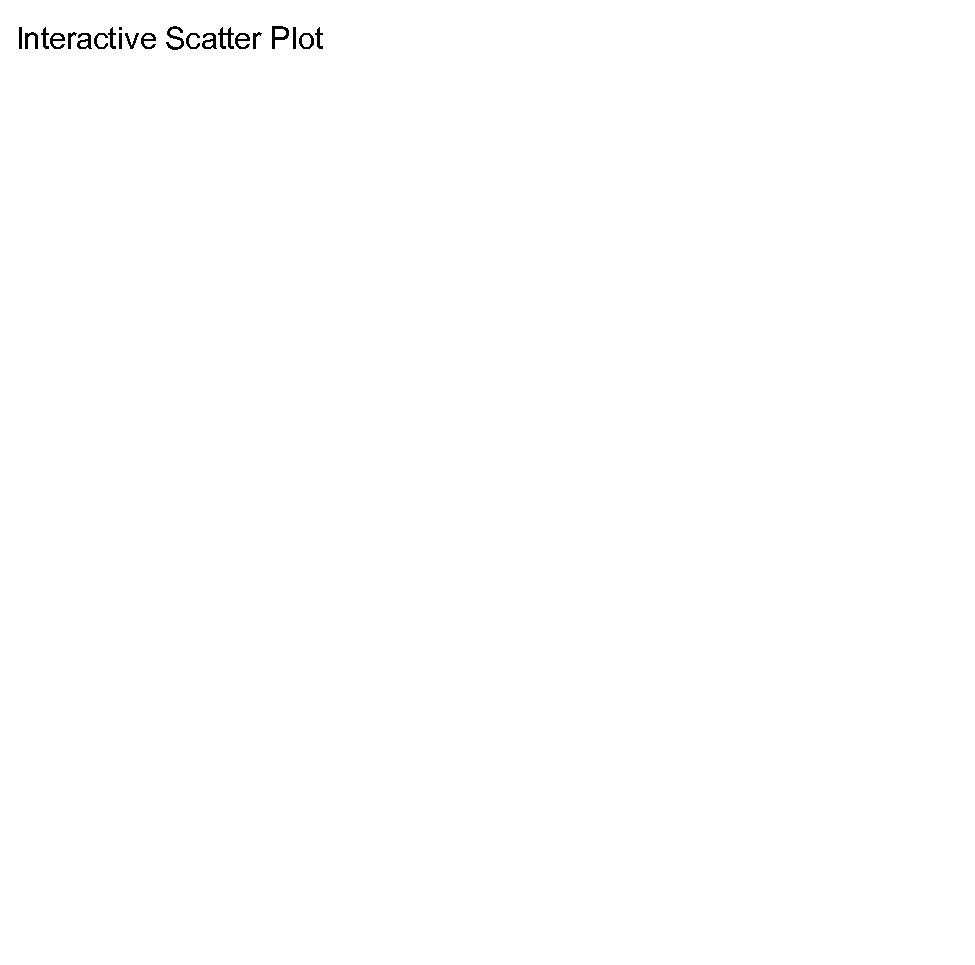
\includegraphics{_main_files/figure-latex/unnamed-chunk-91-1.pdf}

\section{Building Web Applications with shiny}\label{building-web-applications-with-shiny}

\subsection{Introduction to shiny for building interactive web applications}\label{introduction-to-shiny-for-building-interactive-web-applications}

Shiny allows you to turn your analyses into interactive web applications without needing to know HTML, CSS, or JavaScript. It works by allowing you to separate the user interface from the underlying R code, making it easy to create complex interactive apps.

\subsection{Creating reactive plots and dashboards that update with user input.}\label{creating-reactive-plots-and-dashboards-that-update-with-user-input.}

\begin{Shaded}
\begin{Highlighting}[]
\CommentTok{\# Load necessary packages}
\CommentTok{\#library(shiny)}
\CommentTok{\#library(ggplot2)}

\CommentTok{\# Define UI}
\NormalTok{ui }\OtherTok{\textless{}{-}} \FunctionTok{fluidPage}\NormalTok{(}
  \FunctionTok{titlePanel}\NormalTok{(}\StringTok{"Interactive Scatter Plot"}\NormalTok{),}
  \FunctionTok{sidebarLayout}\NormalTok{(}
    \FunctionTok{sidebarPanel}\NormalTok{(}
      \FunctionTok{sliderInput}\NormalTok{(}\StringTok{"slider"}\NormalTok{, }\StringTok{"Number of points to show:"}\NormalTok{, }
                  \AttributeTok{min =} \DecValTok{10}\NormalTok{, }\AttributeTok{max =} \FunctionTok{nrow}\NormalTok{(iris), }\AttributeTok{value =} \DecValTok{50}\NormalTok{)}
\NormalTok{    ),}
    \FunctionTok{mainPanel}\NormalTok{(}
      \FunctionTok{plotOutput}\NormalTok{(}\StringTok{"scatter\_plot"}\NormalTok{)}
\NormalTok{    )}
\NormalTok{  )}
\NormalTok{)}

\CommentTok{\# Define server logic}
\NormalTok{server }\OtherTok{\textless{}{-}} \ControlFlowTok{function}\NormalTok{(input, output) \{}
\NormalTok{  output}\SpecialCharTok{$}\NormalTok{scatter\_plot }\OtherTok{\textless{}{-}} \FunctionTok{renderPlot}\NormalTok{(\{}
\NormalTok{    sample\_rows }\OtherTok{\textless{}{-}} \FunctionTok{sample}\NormalTok{(}\FunctionTok{nrow}\NormalTok{(iris), input}\SpecialCharTok{$}\NormalTok{slider)}
    \FunctionTok{ggplot}\NormalTok{(}\AttributeTok{data =}\NormalTok{ iris[sample\_rows, ], }\FunctionTok{aes}\NormalTok{(}\AttributeTok{x =}\NormalTok{ Sepal.Length, }\AttributeTok{y =}\NormalTok{ Sepal.Width, }\AttributeTok{color =}\NormalTok{ Species)) }\SpecialCharTok{+} 
      \FunctionTok{geom\_point}\NormalTok{() }\SpecialCharTok{+}
      \FunctionTok{labs}\NormalTok{(}\AttributeTok{title =} \StringTok{"Interactive Scatter Plot of Sepal Length vs Sepal Width"}\NormalTok{,}
           \AttributeTok{x =} \StringTok{"Sepal Length"}\NormalTok{, }\AttributeTok{y =} \StringTok{"Sepal Width"}\NormalTok{) }\SpecialCharTok{+}
      \FunctionTok{theme\_minimal}\NormalTok{()}
\NormalTok{  \})}
\NormalTok{\}}

\CommentTok{\# Run the application}
\FunctionTok{shinyApp}\NormalTok{(}\AttributeTok{ui =}\NormalTok{ ui, }\AttributeTok{server =}\NormalTok{ server)}
\end{Highlighting}
\end{Shaded}

\begin{verbatim}
## 
## Listening on http://127.0.0.1:3847
\end{verbatim}

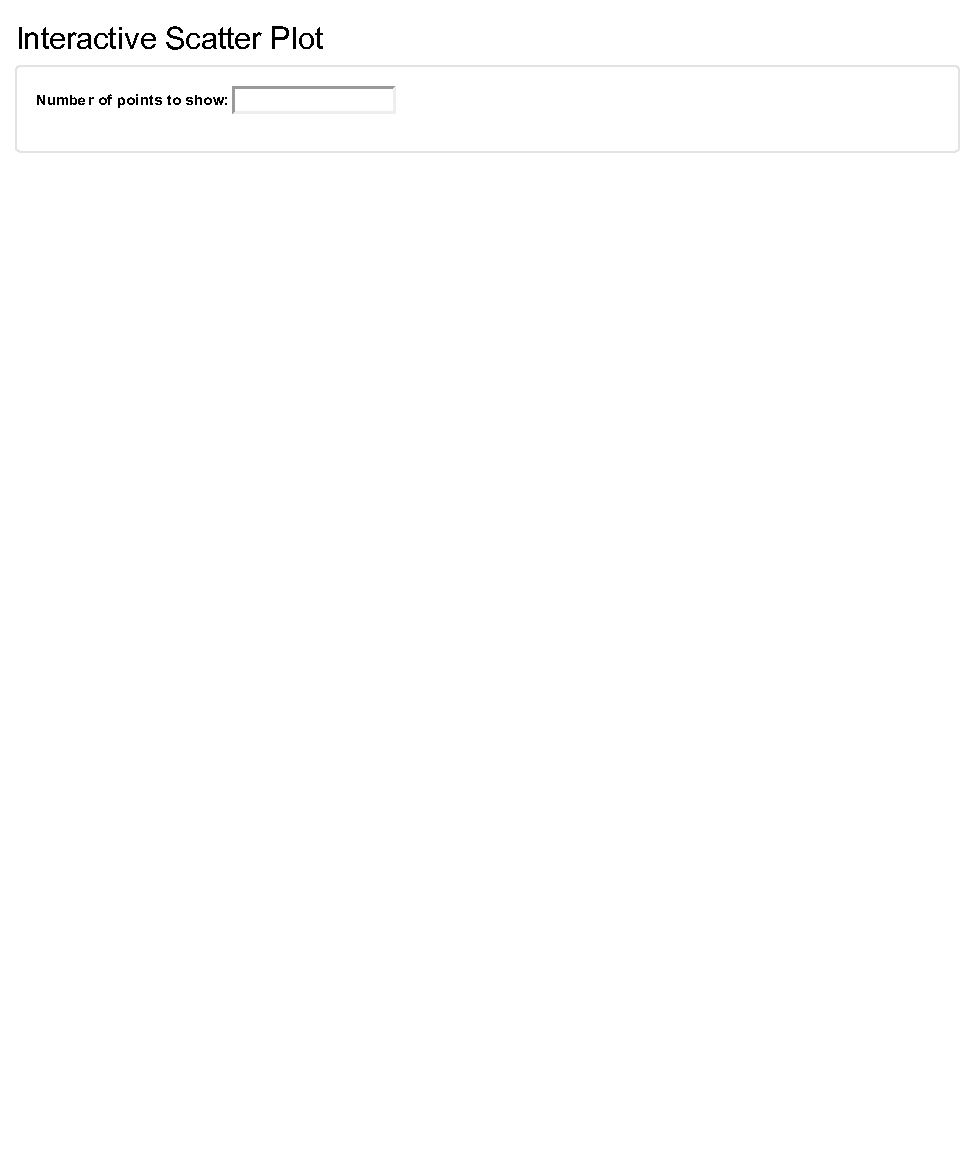
\includegraphics{_main_files/figure-latex/unnamed-chunk-92-1.pdf}

\section{Advanced ggplot2 Extensions}\label{advanced-ggplot2-extensions}

\subsection{Explore extensions like gganimate for creating animated plots.}\label{explore-extensions-like-gganimate-for-creating-animated-plots.}

\begin{Shaded}
\begin{Highlighting}[]
\FunctionTok{library}\NormalTok{(gganimate)}

\CommentTok{\#Note: This plot will be displayed after you install the gifski package}

\CommentTok{\# Animated scatter plot}
\FunctionTok{ggplot}\NormalTok{(iris, }\FunctionTok{aes}\NormalTok{(}\AttributeTok{x =}\NormalTok{ Sepal.Length, }\AttributeTok{y =}\NormalTok{ Sepal.Width, }\AttributeTok{color =}\NormalTok{ Species)) }\SpecialCharTok{+} 
  \FunctionTok{geom\_point}\NormalTok{() }\SpecialCharTok{+}
  \FunctionTok{transition\_states}\NormalTok{(Species, }\AttributeTok{transition\_length =} \DecValTok{2}\NormalTok{, }\AttributeTok{state\_length =} \DecValTok{1}\NormalTok{) }\SpecialCharTok{+}
  \FunctionTok{labs}\NormalTok{(}\AttributeTok{title =} \StringTok{"Animated Scatter Plot of Sepal Length vs Sepal Width"}\NormalTok{,}
       \AttributeTok{x =} \StringTok{"Sepal Length"}\NormalTok{, }\AttributeTok{y =} \StringTok{"Sepal Width"}\NormalTok{) }\SpecialCharTok{+}
  \FunctionTok{theme\_bw}\NormalTok{()}
\end{Highlighting}
\end{Shaded}

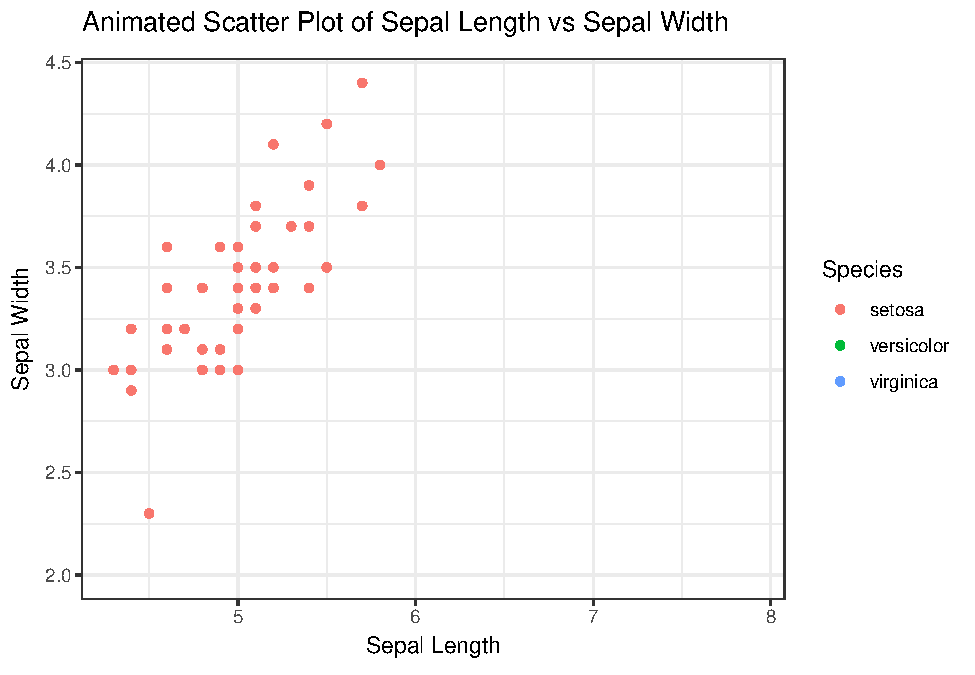
\includegraphics{_main_files/figure-latex/unnamed-chunk-93-1.pdf} 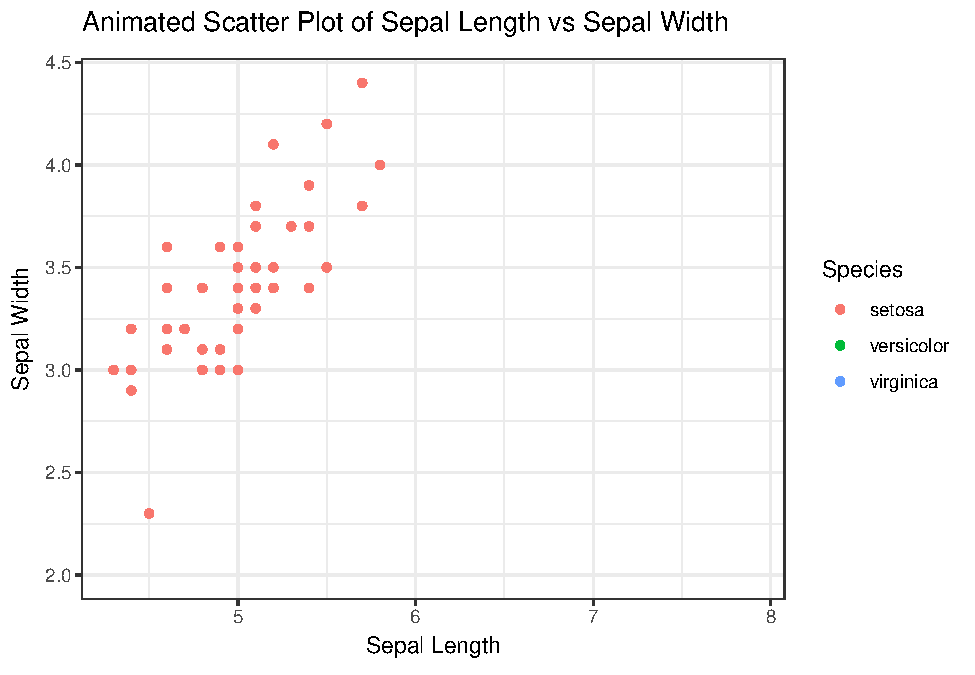
\includegraphics{_main_files/figure-latex/unnamed-chunk-93-2.pdf} 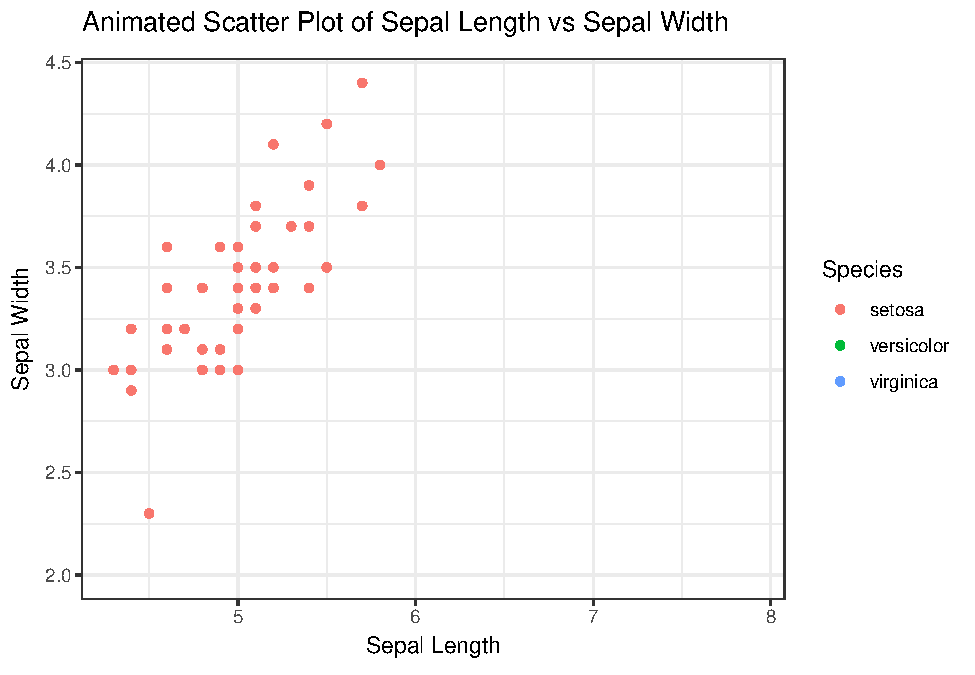
\includegraphics{_main_files/figure-latex/unnamed-chunk-93-3.pdf} \includegraphics{_main_files/figure-latex/unnamed-chunk-93-4.pdf} \includegraphics{_main_files/figure-latex/unnamed-chunk-93-5.pdf} \includegraphics{_main_files/figure-latex/unnamed-chunk-93-6.pdf} \includegraphics{_main_files/figure-latex/unnamed-chunk-93-7.pdf} \includegraphics{_main_files/figure-latex/unnamed-chunk-93-8.pdf} \includegraphics{_main_files/figure-latex/unnamed-chunk-93-9.pdf} \includegraphics{_main_files/figure-latex/unnamed-chunk-93-10.pdf} \includegraphics{_main_files/figure-latex/unnamed-chunk-93-11.pdf} \includegraphics{_main_files/figure-latex/unnamed-chunk-93-12.pdf} \includegraphics{_main_files/figure-latex/unnamed-chunk-93-13.pdf} \includegraphics{_main_files/figure-latex/unnamed-chunk-93-14.pdf} \includegraphics{_main_files/figure-latex/unnamed-chunk-93-15.pdf} \includegraphics{_main_files/figure-latex/unnamed-chunk-93-16.pdf} \includegraphics{_main_files/figure-latex/unnamed-chunk-93-17.pdf} \includegraphics{_main_files/figure-latex/unnamed-chunk-93-18.pdf} \includegraphics{_main_files/figure-latex/unnamed-chunk-93-19.pdf} \includegraphics{_main_files/figure-latex/unnamed-chunk-93-20.pdf} \includegraphics{_main_files/figure-latex/unnamed-chunk-93-21.pdf} \includegraphics{_main_files/figure-latex/unnamed-chunk-93-22.pdf} \includegraphics{_main_files/figure-latex/unnamed-chunk-93-23.pdf} \includegraphics{_main_files/figure-latex/unnamed-chunk-93-24.pdf} \includegraphics{_main_files/figure-latex/unnamed-chunk-93-25.pdf} \includegraphics{_main_files/figure-latex/unnamed-chunk-93-26.pdf} \includegraphics{_main_files/figure-latex/unnamed-chunk-93-27.pdf} \includegraphics{_main_files/figure-latex/unnamed-chunk-93-28.pdf} \includegraphics{_main_files/figure-latex/unnamed-chunk-93-29.pdf} \includegraphics{_main_files/figure-latex/unnamed-chunk-93-30.pdf} \includegraphics{_main_files/figure-latex/unnamed-chunk-93-31.pdf} \includegraphics{_main_files/figure-latex/unnamed-chunk-93-32.pdf} \includegraphics{_main_files/figure-latex/unnamed-chunk-93-33.pdf} \includegraphics{_main_files/figure-latex/unnamed-chunk-93-34.pdf} \includegraphics{_main_files/figure-latex/unnamed-chunk-93-35.pdf} \includegraphics{_main_files/figure-latex/unnamed-chunk-93-36.pdf} \includegraphics{_main_files/figure-latex/unnamed-chunk-93-37.pdf} \includegraphics{_main_files/figure-latex/unnamed-chunk-93-38.pdf} \includegraphics{_main_files/figure-latex/unnamed-chunk-93-39.pdf} \includegraphics{_main_files/figure-latex/unnamed-chunk-93-40.pdf} \includegraphics{_main_files/figure-latex/unnamed-chunk-93-41.pdf} \includegraphics{_main_files/figure-latex/unnamed-chunk-93-42.pdf} \includegraphics{_main_files/figure-latex/unnamed-chunk-93-43.pdf} \includegraphics{_main_files/figure-latex/unnamed-chunk-93-44.pdf} \includegraphics{_main_files/figure-latex/unnamed-chunk-93-45.pdf} \includegraphics{_main_files/figure-latex/unnamed-chunk-93-46.pdf} \includegraphics{_main_files/figure-latex/unnamed-chunk-93-47.pdf} \includegraphics{_main_files/figure-latex/unnamed-chunk-93-48.pdf} \includegraphics{_main_files/figure-latex/unnamed-chunk-93-49.pdf} \includegraphics{_main_files/figure-latex/unnamed-chunk-93-50.pdf} \includegraphics{_main_files/figure-latex/unnamed-chunk-93-51.pdf} \includegraphics{_main_files/figure-latex/unnamed-chunk-93-52.pdf} \includegraphics{_main_files/figure-latex/unnamed-chunk-93-53.pdf} \includegraphics{_main_files/figure-latex/unnamed-chunk-93-54.pdf} \includegraphics{_main_files/figure-latex/unnamed-chunk-93-55.pdf} \includegraphics{_main_files/figure-latex/unnamed-chunk-93-56.pdf} \includegraphics{_main_files/figure-latex/unnamed-chunk-93-57.pdf} \includegraphics{_main_files/figure-latex/unnamed-chunk-93-58.pdf} \includegraphics{_main_files/figure-latex/unnamed-chunk-93-59.pdf} \includegraphics{_main_files/figure-latex/unnamed-chunk-93-60.pdf} \includegraphics{_main_files/figure-latex/unnamed-chunk-93-61.pdf} \includegraphics{_main_files/figure-latex/unnamed-chunk-93-62.pdf} \includegraphics{_main_files/figure-latex/unnamed-chunk-93-63.pdf} \includegraphics{_main_files/figure-latex/unnamed-chunk-93-64.pdf} \includegraphics{_main_files/figure-latex/unnamed-chunk-93-65.pdf} \includegraphics{_main_files/figure-latex/unnamed-chunk-93-66.pdf} \includegraphics{_main_files/figure-latex/unnamed-chunk-93-67.pdf} \includegraphics{_main_files/figure-latex/unnamed-chunk-93-68.pdf} \includegraphics{_main_files/figure-latex/unnamed-chunk-93-69.pdf} \includegraphics{_main_files/figure-latex/unnamed-chunk-93-70.pdf} \includegraphics{_main_files/figure-latex/unnamed-chunk-93-71.pdf} \includegraphics{_main_files/figure-latex/unnamed-chunk-93-72.pdf} \includegraphics{_main_files/figure-latex/unnamed-chunk-93-73.pdf} \includegraphics{_main_files/figure-latex/unnamed-chunk-93-74.pdf} \includegraphics{_main_files/figure-latex/unnamed-chunk-93-75.pdf} \includegraphics{_main_files/figure-latex/unnamed-chunk-93-76.pdf} \includegraphics{_main_files/figure-latex/unnamed-chunk-93-77.pdf} \includegraphics{_main_files/figure-latex/unnamed-chunk-93-78.pdf} \includegraphics{_main_files/figure-latex/unnamed-chunk-93-79.pdf} \includegraphics{_main_files/figure-latex/unnamed-chunk-93-80.pdf} \includegraphics{_main_files/figure-latex/unnamed-chunk-93-81.pdf} \includegraphics{_main_files/figure-latex/unnamed-chunk-93-82.pdf} \includegraphics{_main_files/figure-latex/unnamed-chunk-93-83.pdf} \includegraphics{_main_files/figure-latex/unnamed-chunk-93-84.pdf} \includegraphics{_main_files/figure-latex/unnamed-chunk-93-85.pdf} \includegraphics{_main_files/figure-latex/unnamed-chunk-93-86.pdf} \includegraphics{_main_files/figure-latex/unnamed-chunk-93-87.pdf} \includegraphics{_main_files/figure-latex/unnamed-chunk-93-88.pdf} \includegraphics{_main_files/figure-latex/unnamed-chunk-93-89.pdf} \includegraphics{_main_files/figure-latex/unnamed-chunk-93-90.pdf} \includegraphics{_main_files/figure-latex/unnamed-chunk-93-91.pdf} \includegraphics{_main_files/figure-latex/unnamed-chunk-93-92.pdf} \includegraphics{_main_files/figure-latex/unnamed-chunk-93-93.pdf} \includegraphics{_main_files/figure-latex/unnamed-chunk-93-94.pdf} \includegraphics{_main_files/figure-latex/unnamed-chunk-93-95.pdf} \includegraphics{_main_files/figure-latex/unnamed-chunk-93-96.pdf} \includegraphics{_main_files/figure-latex/unnamed-chunk-93-97.pdf} \includegraphics{_main_files/figure-latex/unnamed-chunk-93-98.pdf} \includegraphics{_main_files/figure-latex/unnamed-chunk-93-99.pdf} \includegraphics{_main_files/figure-latex/unnamed-chunk-93-100.pdf}

\subsection{Using ggridges for ridge line plots and other creative visualization techniques.}\label{using-ggridges-for-ridge-line-plots-and-other-creative-visualization-techniques.}

\begin{Shaded}
\begin{Highlighting}[]
\FunctionTok{library}\NormalTok{(ggridges)}

\CommentTok{\# Ridge line plot}
\FunctionTok{ggplot}\NormalTok{(iris, }\FunctionTok{aes}\NormalTok{(}\AttributeTok{x =}\NormalTok{ Sepal.Length, }\AttributeTok{y =}\NormalTok{ Species, }\AttributeTok{fill =}\NormalTok{ Species)) }\SpecialCharTok{+} 
  \FunctionTok{geom\_density\_ridges}\NormalTok{() }\SpecialCharTok{+}
  \FunctionTok{labs}\NormalTok{(}\AttributeTok{title =} \StringTok{"Ridge Line Plot of Sepal Length by Species"}\NormalTok{,}
       \AttributeTok{x =} \StringTok{"Sepal Length"}\NormalTok{, }\AttributeTok{y =} \StringTok{"Species"}\NormalTok{) }\SpecialCharTok{+}
  \FunctionTok{theme\_bw}\NormalTok{()}
\end{Highlighting}
\end{Shaded}

\includegraphics{_main_files/figure-latex/unnamed-chunk-94-1.pdf}

\section{Practical Examples: Exercises}\label{practical-examples-exercises-4}

\chapter{REAL-WORLD APPLICATIONS AND CASE STUDIES (CODE CHALLENGES)}\label{real-world-applications-and-case-studies-code-challenges}

\end{document}
